\documentclass[sigconf]{acmart}

\def\BibTeX{{\rm B\kern-.05em{\sc i\kern-.025em b}\kern-.08emT\kern-.1667em\lower.7ex\hbox{E}\kern-.125emX}}
\usepackage{subfigure}
\usepackage{algorithm}
%\usepackage{algorithmic}
\usepackage{algpseudocode}
\usepackage{amsmath}
\usepackage{graphics}
\usepackage{epsfig}
\usepackage{multirow}
\usepackage{graphicx}
\usepackage{subfigure}
\usepackage{array}

\begin{document}

\title{Approximate Code: A Cost-Effective Erasure Coding Framework for Tiered Video Storage in Cloud Systems}

\author{Huayi Jin, Chentao Wu, Xin Xie, Jie Li, Minyi Guo, Hao Lin, Jianfeng Zhang}
%\email{keplar_gd@sjtu.edu.cn}
\affiliation{%
    \institution{Shanghai Jiao Tong University}
    \institution{The Alibaba Group}
}

\begin{abstract}
Nowadays massive video data are stored in cloud storage systems, which are generated by various applications such as autonomous driving, news media, security monitoring, etc. Meanwhile, erasure coding is a popular technique in cloud storage to provide both high reliability with low monetary cost, where triple disk failure tolerant arrays (3DFTs) is a typical choice. Therefore, how to minimize the storage cost of video data in 3DFTs is challenge for cloud storage systems. Although there are several solutions like approximate storage technique, they cannot guarantee low storage cost and high data reliability concurrently.

To address this challenge, in this paper, we propose Approximate Code, which is an erasure coding framework for tiered video storage in cloud systems. The key idea of Approximate Code is distinguishing the important and unimportant data with different capabilities of fault tolerance. On one hand, for important data, Approximate Code provides triple parities to provide high reliability. On the other hand, single/double parities are applied for unimportant data, which can save the storage cost and accelerate the recovery process. To demonstrate the effectiveness of Approximate Code, we conduct several experiments in Hadoop systems. The results show that, compared to traditional 3DFTs using various erasure codes such as RS, LRC, STAR and TIP-Code, Approximate Code reduces the number of parities by up to 55\%, saves the storage cost by up to 20.8\% and increase the recovery speed by up to 1.25X when double disks fail.
\end{abstract}

\ccsdesc[500]{Information systems~Distributed storage}
\ccsdesc[500]{Computer systems organization~Dependable and fault-tolerant systems and networks}

\keywords{Erasure Codes, Approximate Storage, Multimedia, Cloud Storage}
\maketitle

\section{Introduction}
For typical cloud storage systems such as Windows Azure \cite{calder2011windows} and Amazon AWS \cite{bermudez2013exploring}, erasure coding is a popular technique to provide both high reliability and low monetary cost \cite{EVENODD, RDP, BlaumRoth, XCode, CRS, TripleStar, TPtech, RSL}, where triple disk failure fault tolerant arrays (3DFTs) are widely used. Typical erasure codes can be divided into two categories, RS-based Codes \cite{RS} \cite{LRC} and XOR-based codes \cite{EVENODD, hcode, STAR, tip}. RS-based codes are encoded according the Galois Field(GF) Computation \cite{RS}, which allow flexible configuration and have a little higher computation cost. XOR-based codes simplify the computation, but they suffer other issues like scalability. \textcolor{red}{[CITE GSR SDM]}

With the increasing demand on higher resolution and frame rate for video data, massive storage devices are highly desired in cloud storage systems, which makes data centers much bigger.
Therefore, in this paper, we set out to answer the following question:

\textbf{In a cloud storage system, how to efficiently store tremendous video data in 3DFTs?}

To reduce the storage cost in cloud storage systems, a feasible solution is approximate storage. Approximate storage exposes unimportant data to errors, saving the overhead of redundant backups \cite{niklaus2018context, sampson2014approximate} , thus the data reliability cannot be guaranteed.
The second solution is using disk arrays like RAID-5 or RAID-6 \cite{RAID}, but the capability of fault tolerance are sacrificed.
Data compression\footnote{Typically, video coding (e.g., H.264 \cite{wiegand2003overview}) is a special type of data compression.}
is the third strategy to reduce the storage overhead \cite{ziv1977universal, ziv1978compression, deutsch1996deflate}, which needs to be collaborated with erasure codes for high reliability. However, the compression/decompression processes result in a large amount of computational overhead, which limits their usage in cloud systems. 
Therefore, existing solutions are difficult to provide low storage cost and high reliability simultaneously.

To address the above challenge, in this paper, we propose Approximate Code, which is an erasure coding framework to provide comprehensive solution for tiered video data storage in cloud systems. The key idea of Approximate Code is treating the important/unimportant data in different ways. For important data, we add additional parities to provide high capability of fault tolerance. On the other hand, the unimportant data are encoded with a minimum number of parities, which only supply the basic requirement of the recovery. When triple disks fail, the lost unimportant data can be reconstructed via a fuzzy manner.

We have the following contributions of this work,
\begin{enumerate}
\item We propose Approximate Code, which a cost-effective framework to store video data in cloud storage systems.
\item Approximate Code can be implemented by combining various erasure codes in 3DFTs, such as RS, STAR Code, TIP-Code, etc.
\item We conduct several quantitative analysis, simulations and experiments according to different layouts of various erasure codes, and the results show that Approximate Code achieves a small number of parities, low storage cost, high single write performance, and fast data recovery under various failure scenarios.
\end{enumerate}

The rest of the paper is organized as follows. In Section \ref{RelatedWork}, we introduce related work and our motivation.
In Section \ref{ApCode}, the design of Approximate Code and its encoding and decoding process will be illustrated in detail.
%Section \ref{Implementation} introduce the implementation of our design, and section \ref{ap-recovery} analysis the performance of approximate video storage.
The evaluation is presented in Section \ref{evaluation} and the conclusion of our work is in Section \ref{Conclusion}.

\section{Related Work and Our Motivation}\label{RelatedWork}
In this section, we introduce the background of video storage, existing solutions to reduce storage cost and the motivation of this paper.
To facilitate the discussion, we summarize the symbols used in this paper in Table \ref{parameter}.

\begin{table}[]\footnotesize
\caption{The symbols used in this paper.}\label{parameter}
\centering
\begin{tabular}{|p{0.7cm}<{\centering}|p{6.5cm}|}
\hline
Symbols & \multicolumn{1}{c|}{Description} \\ \hline \hline
$k$ & the number of data nodes in a local stripe \\ \hline
$r$ & the number of local parity nodes in a local stripe \\ \hline
$n$ & the number of all data and parity nodes in a local stripe. ($n=k+r$) \\ \hline
$h$ & the number of local stripes to construct a global stripe \\ \hline
$g$ & the number of global parity nodes \\ \hline
$N$ & total number of all nodes ($N=(k+r)h+g$) \\ \hline
$C_{i,j}$ & the element at the $i$-th row and $j$-th column \\ \hline
$A_{i,j}$ &  the coefficient of $C_{ij}$ in the Galois Field \\ \hline
$D_i$ & a data node \\ \hline
$P_{I}$ & the mathematical expectation of important data being recoverable under faults that exceed fault tolerance \\ \hline
$P_{U}$ & the mathematical expectation of unimportant data being recoverable under faults that exceed fault tolerance \\ \hline
$\oplus$ & the XOR operation symbol \\ \hline
$\binom{n}{k}$ & The number of $k$-combinations from $n$ elements\\ \hline
LP & local parity nodes \\ \hline
GP & global parity nodes \\ \hline
ID & important data in a video file \\ \hline
UD & unimportant data in a video file \\ \hline
\end{tabular}
\vspace{-3mm}
\end{table}


\subsection{Basis of Video Storage}\label{video storage}
For normal HD (resolution 1280$\times$720, 8-bit, 30 fps) video, the amount of raw video data in 1 minute is 4.63 GB, so video data is usually encoded by lossy compression algorithms before storage.

\subsubsection{Video coding}
H.264 \cite{wiegand2003overview} is one of the advanced algorithms. This coding technique is widely used on platforms such as YouTube because it has higher compression ratio and lower complexity than its predecessor. For a normal HD video file as mentioned above, H.264 can reduce its size by about 10 times, only 443.27MB.

H.264 classifies all frames into three different categories:
\begin{enumerate}
    \item I frame: A frame that is self-contained, which means it can be decoded independently.
    \item P frame: A frame holds the changes compared to the previous frame, which saves the storage space by leaving out redundant information.
    \item B frame: A frame decreases the storage space as well by utilizing the data of both the preceding and following frames.
\end{enumerate}
A group of pictures (GOP) consists of one I frame followed by a number of consecutive P and B frames, as shown in Figure \ref{H264-IPB}.
Within each GOP, the I frame is the most significant because all other frames rely on if for recovery. P frames are the second important, and B frames have the least value.
Based on this feature, a special program can be designed to distinguish the importance of video frames.

\begin{figure}[ht]
\centering
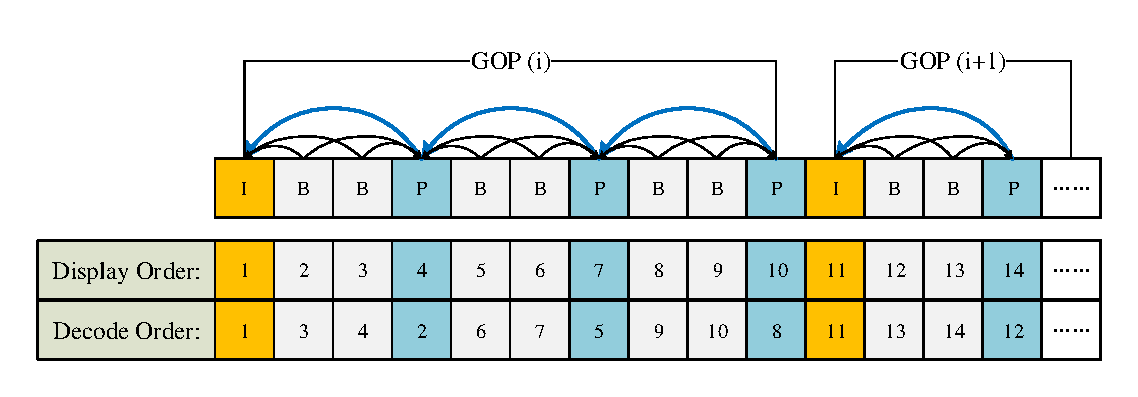
\includegraphics[width=0.4\textwidth]{photo/H264_IPB.pdf}
\vspace{-3mm}
\caption{A sample of GOPs in H.264}
\vspace{-3mm}
\label{H264-IPB}
\end{figure}

\subsubsection{Video Frame Recovery}
In the circumstance of video approximate storage, it's common to lose some frames and leave the video incomplete. However, the lost frames can still be recoverable with the benefit of powerful deep learning techniques. One of them is named video frame interpolation \cite{meyer2015phase, niklaus2018context, van2017frame}.

Video frame interpolation is one of the basic video processing techniques, an attempt to synthetically produce one or more intermediate video frames from existing ones. This is a technique that can model natural motion within a video, and generate frames according to the model.

\subsection{Existing Erasure Codes}\label{existEC}

Reliability is a critical issue since disk failures are typical in storage systems. To improve the reliability of storage systems, several RAID forms (e.g., RAID-5, RAID-6, 3DFTs) and erasure codes are proposed by researchers.  Traditional erasure codes can be categorized into two classes, Maximum Distance Separable (MDS) codes and non-MDS codes. MDS codes aim to offer data protection with optimal storage efficiency. On the other hand, non-MDS codes improve the performance or reliability by consuming extra storage space.

In the past two decades, several famous erasure codes are proposed for double Disk Failure Tolerant arrays (2DFTs or RAID-6), such as EVENODD code \cite{EVENODD}, RDP code \cite{RDP}, Blaum-Roth code\cite{BlaumRoth}, X-code \cite{XCode}, Liberation code \cite{Liberation}, Liber8tion code \cite{Liber8tion}, Cyclic \cite {Cyclic} code, B-Code \cite{BCode}, Code-M \cite{Code-M}, H-code \cite{hcode}, P-code \cite{PCode} and HVcode \cite{HVCode}, etc.

In Triple Disks Failure Tolerant Arrays (3DFTs), typical MDS codes include Reed-Solomon codes \cite{RS}, Cauchy-RS codes \cite{CRS}, STAR code \cite{STAR}, Triple-Star code \cite{TripleStar}, Triple-Parity code \cite{TPtech}, HDD1 code \cite{HDD}, RSL-code \cite{RSL}, RL-code \cite{RL}, and so on. Typical non-MDS codes contain WEAVER codes \cite{WEAVER}, HoVercodes \cite{HoVer}, T-code \cite{TCode}, HDD2 code \cite{HDD}, Pyramid codes \cite{Pyramid}, Local Reconstruction Codes \cite{LRC}, Locally Repairable Codes \cite{XORing}, etc.
In the following we mainly introduce the classic erasure codes used in this paper.

Reed Solomon (RS) Code \cite{RS} is a classic MDS code, as shown in Figure \ref{fig-RS-1}. The encoding and decoding operations of RS code are based on Galois Field (GF), leading to high scalability as well as high computational complexity.

Local Construction Code (LRC) \cite{LRC} 
is shown in Figure \ref{fig-LRC-1}. It divides the data nodes into several groups, which are called local stripes. Typically, each local stripe contains one local parity node, which is calculated via the data nodes in the same stripe. Global stripe is generated via crossing multiple local stripes.

\begin{figure}
\centering
\subfigure[RS Code for arbitrary storage nodes ($k=4, r=3$). The figure shows the encoding of different horizontal parities. (e.g., $C_{0,5} = \sum_{i=0}^3 A_{0,i}C_{0,i}$)]{
    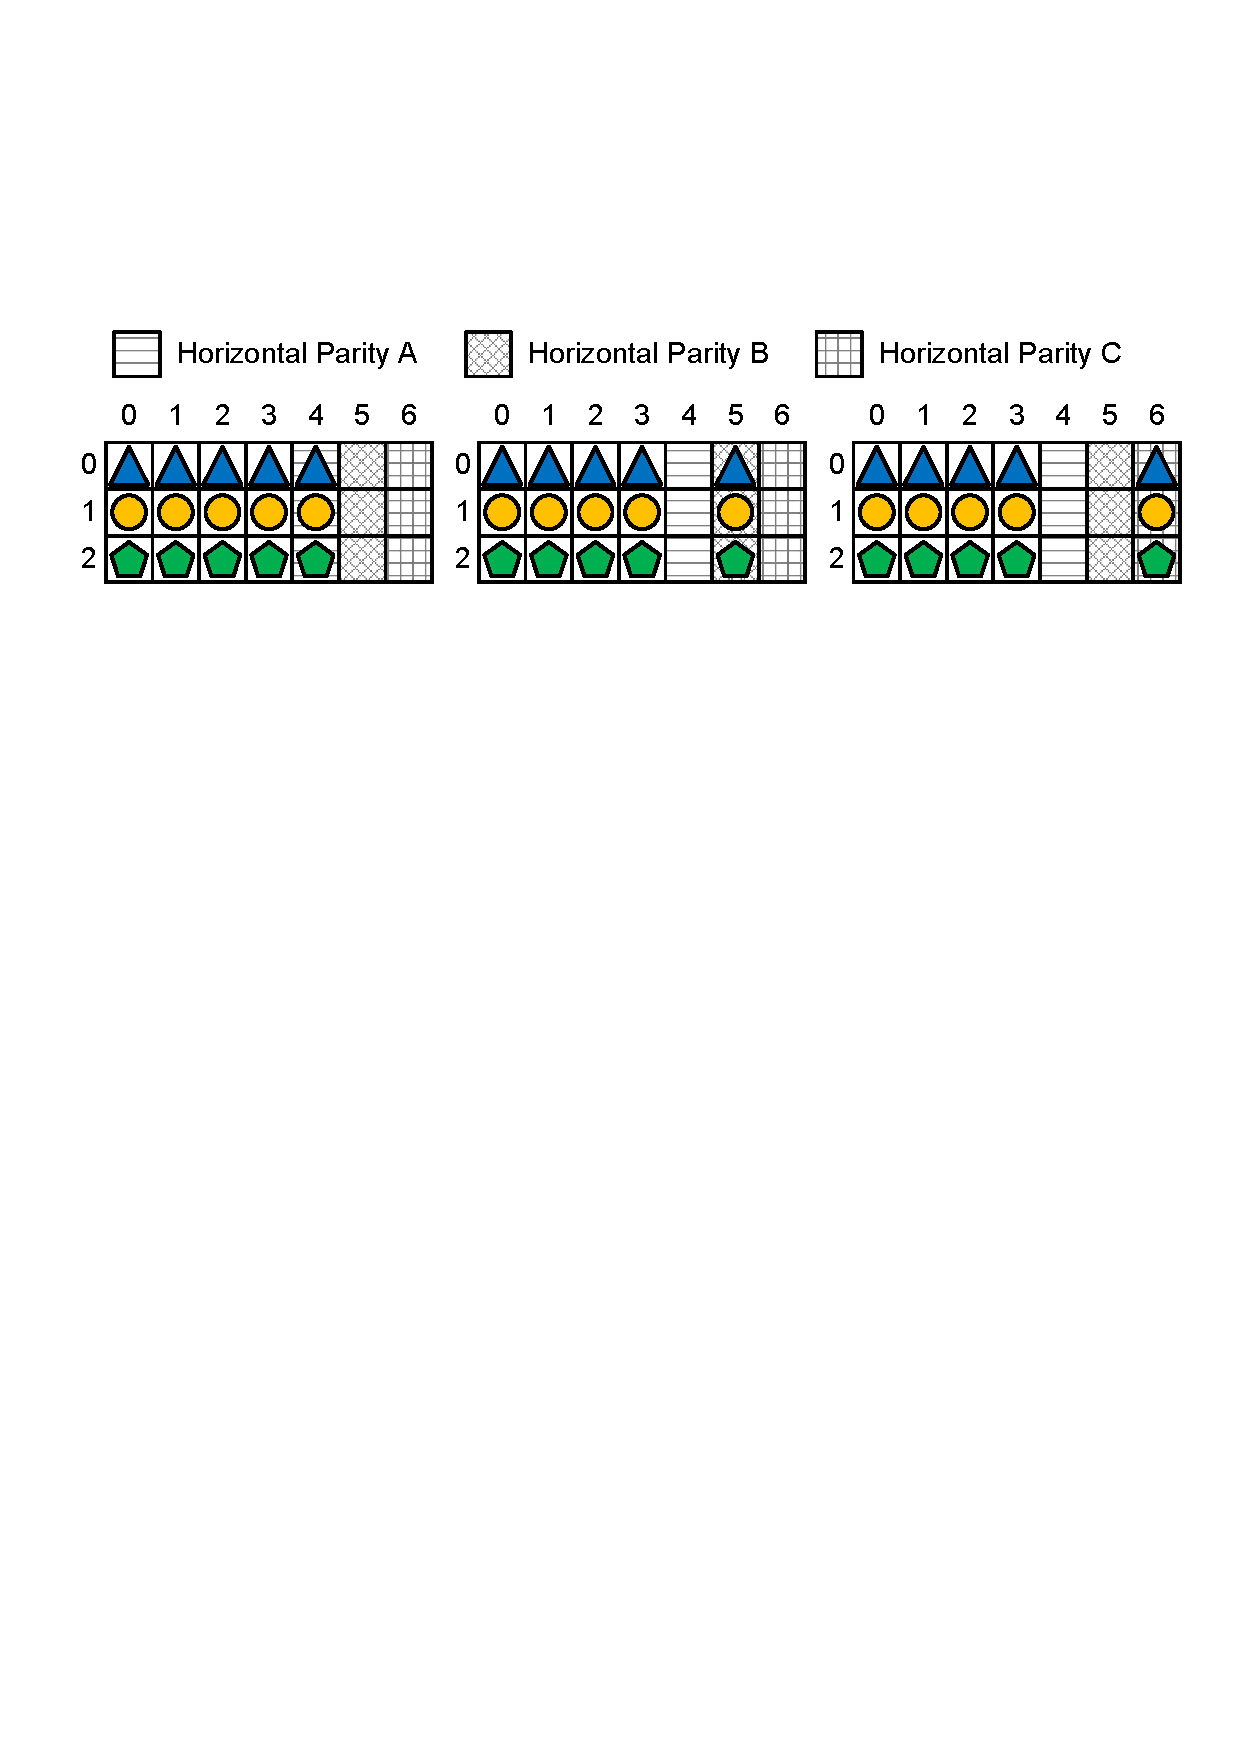
\includegraphics[width=0.92\linewidth]{photo/RS-1.pdf}\label{fig-RS-1}
}

\subfigure[LRC Code for arbitrary storage nodes ($k=4, r=2, g=2$), where 4 nodes are divided into 2 local groups and each of them has a local parity.The figure shows the encoding of local and global parities. (e.g., the local parity $C_{0,5} = \sum_{i=2}^3 A_{0,i}C_{0,i}$ and the global parity $C_{0,7} = \sum_{i=0}^3 A_{0,i}C_{0,i}$)]{
    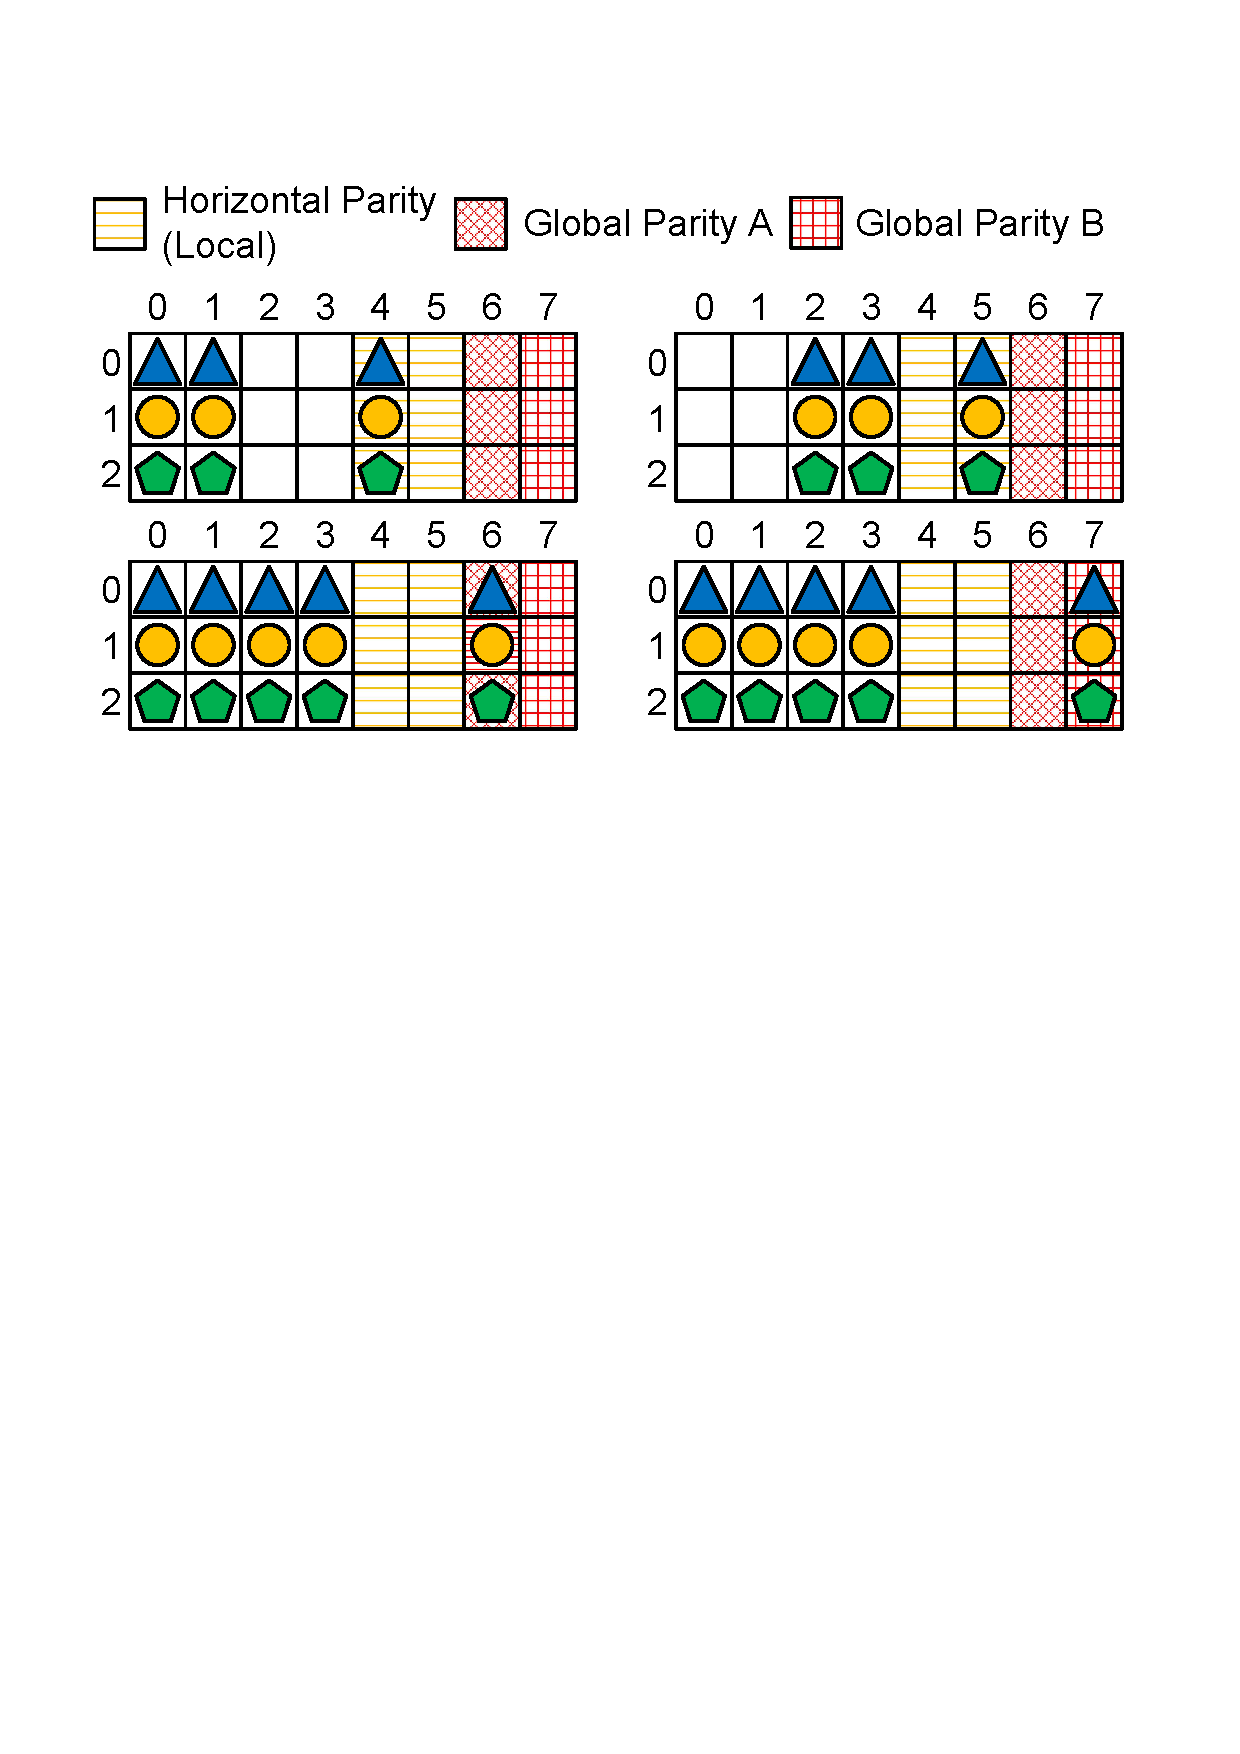
\includegraphics[width=0.8\linewidth]{photo/LRC-1.pdf}\label{fig-LRC-1}
}\vspace{-3mm}
\caption{Encoding of RS code and LRC}
\vspace{-3mm}
\end{figure}

STAR code \cite{STAR} is an extension of EVENODD \cite{EVENODD} code, as shown in Figure \ref{fig-star-tip}.
In the encoding process of STAR code, the generation of diagonal parity and anti-diagonal parity requires to calculate $S1$ and $S2$ first, which lead to a long parity chain.

\begin{figure}[!ht]
\centering
\subfigure[\textbf{STAR Code:} Horizontal parity coding (e.g., $C_{0,5} = C_{0,0} \oplus C_{0,1} \oplus C_{0,2} \oplus C_{0,3} \oplus C_{0,4}$).]{
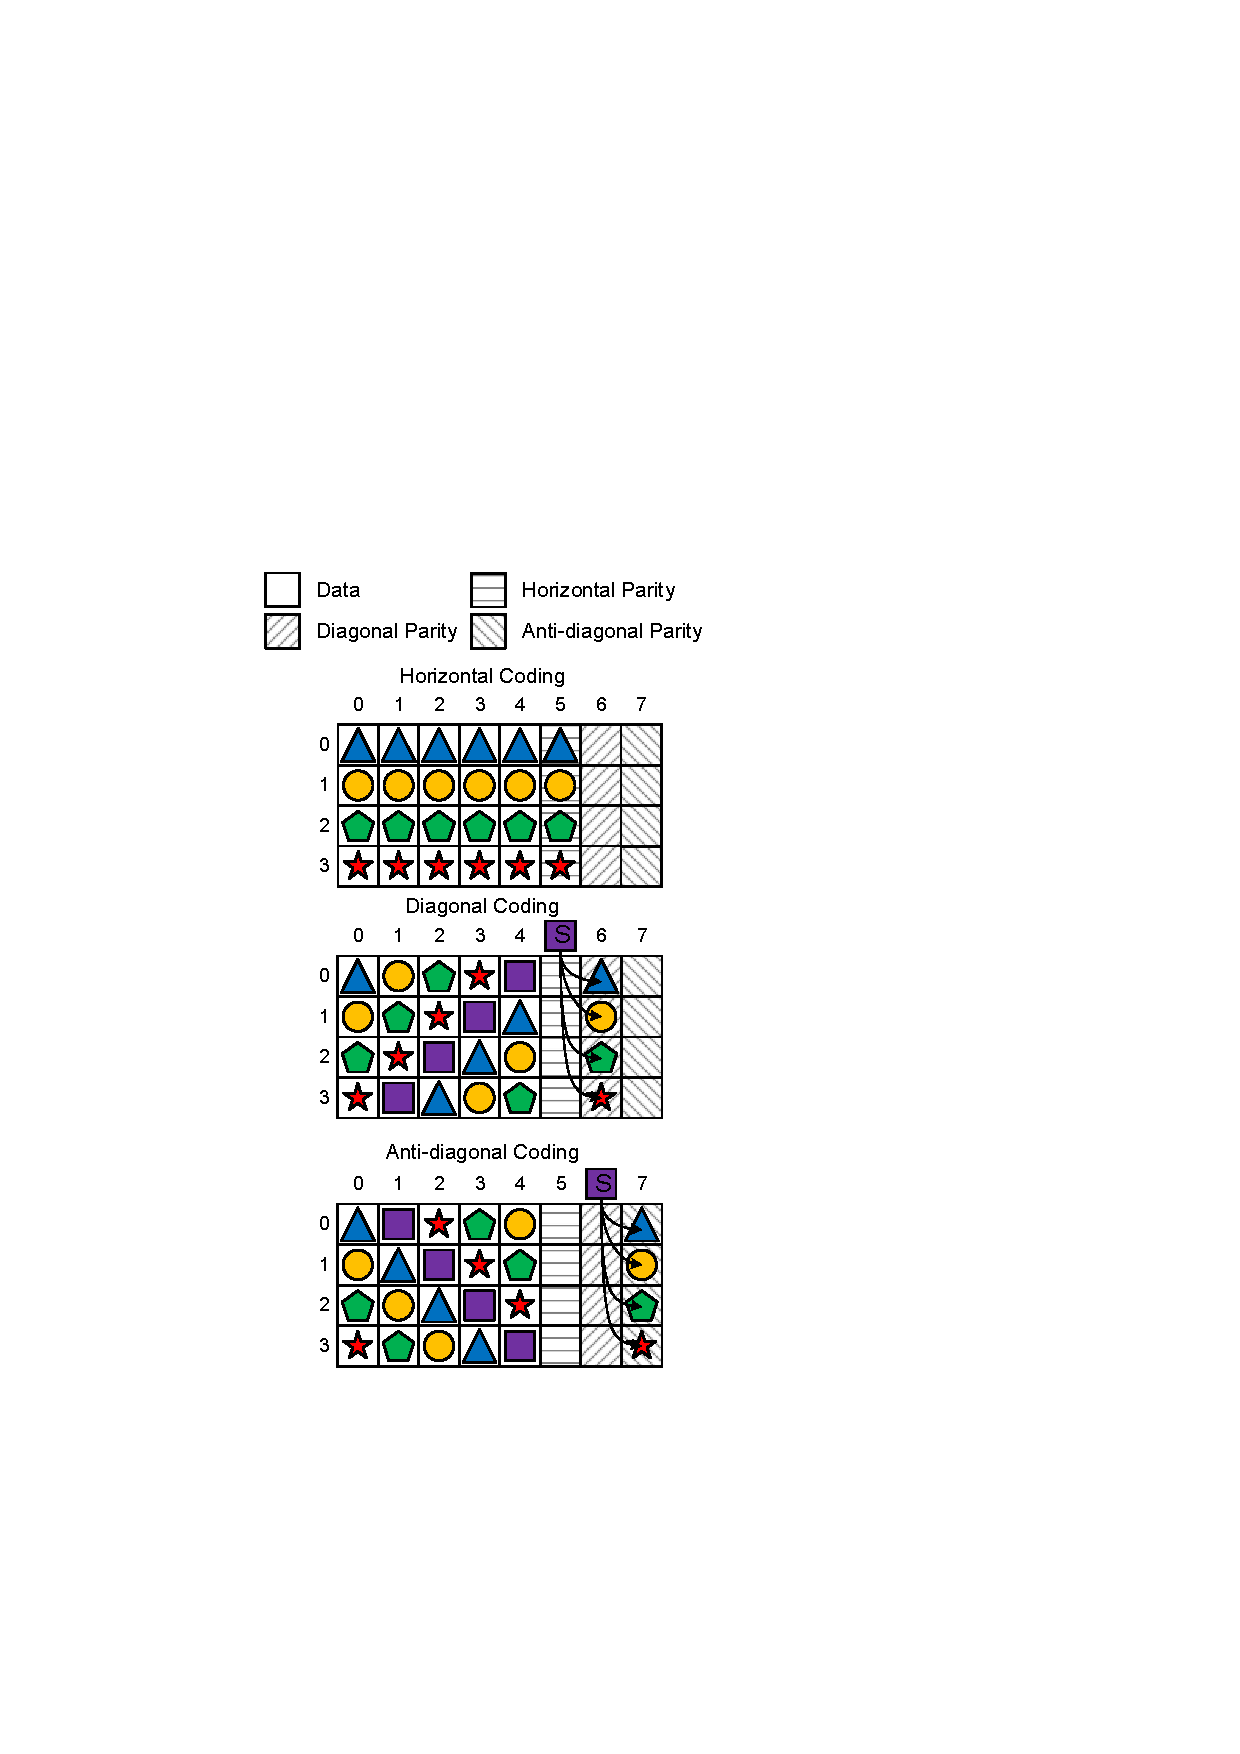
\includegraphics[height=6cm]{photo/STAR.pdf}\label{fig-star}
}
\hspace{5pt}
\subfigure[\textbf{TIP-Code:} Anti-diagonal parity coding (e.g., $C_{0,6} = C_{0,0} \oplus C_{1,1} \oplus C_{2,2} \oplus C_{4,4} \oplus C_{5,5}$).]{
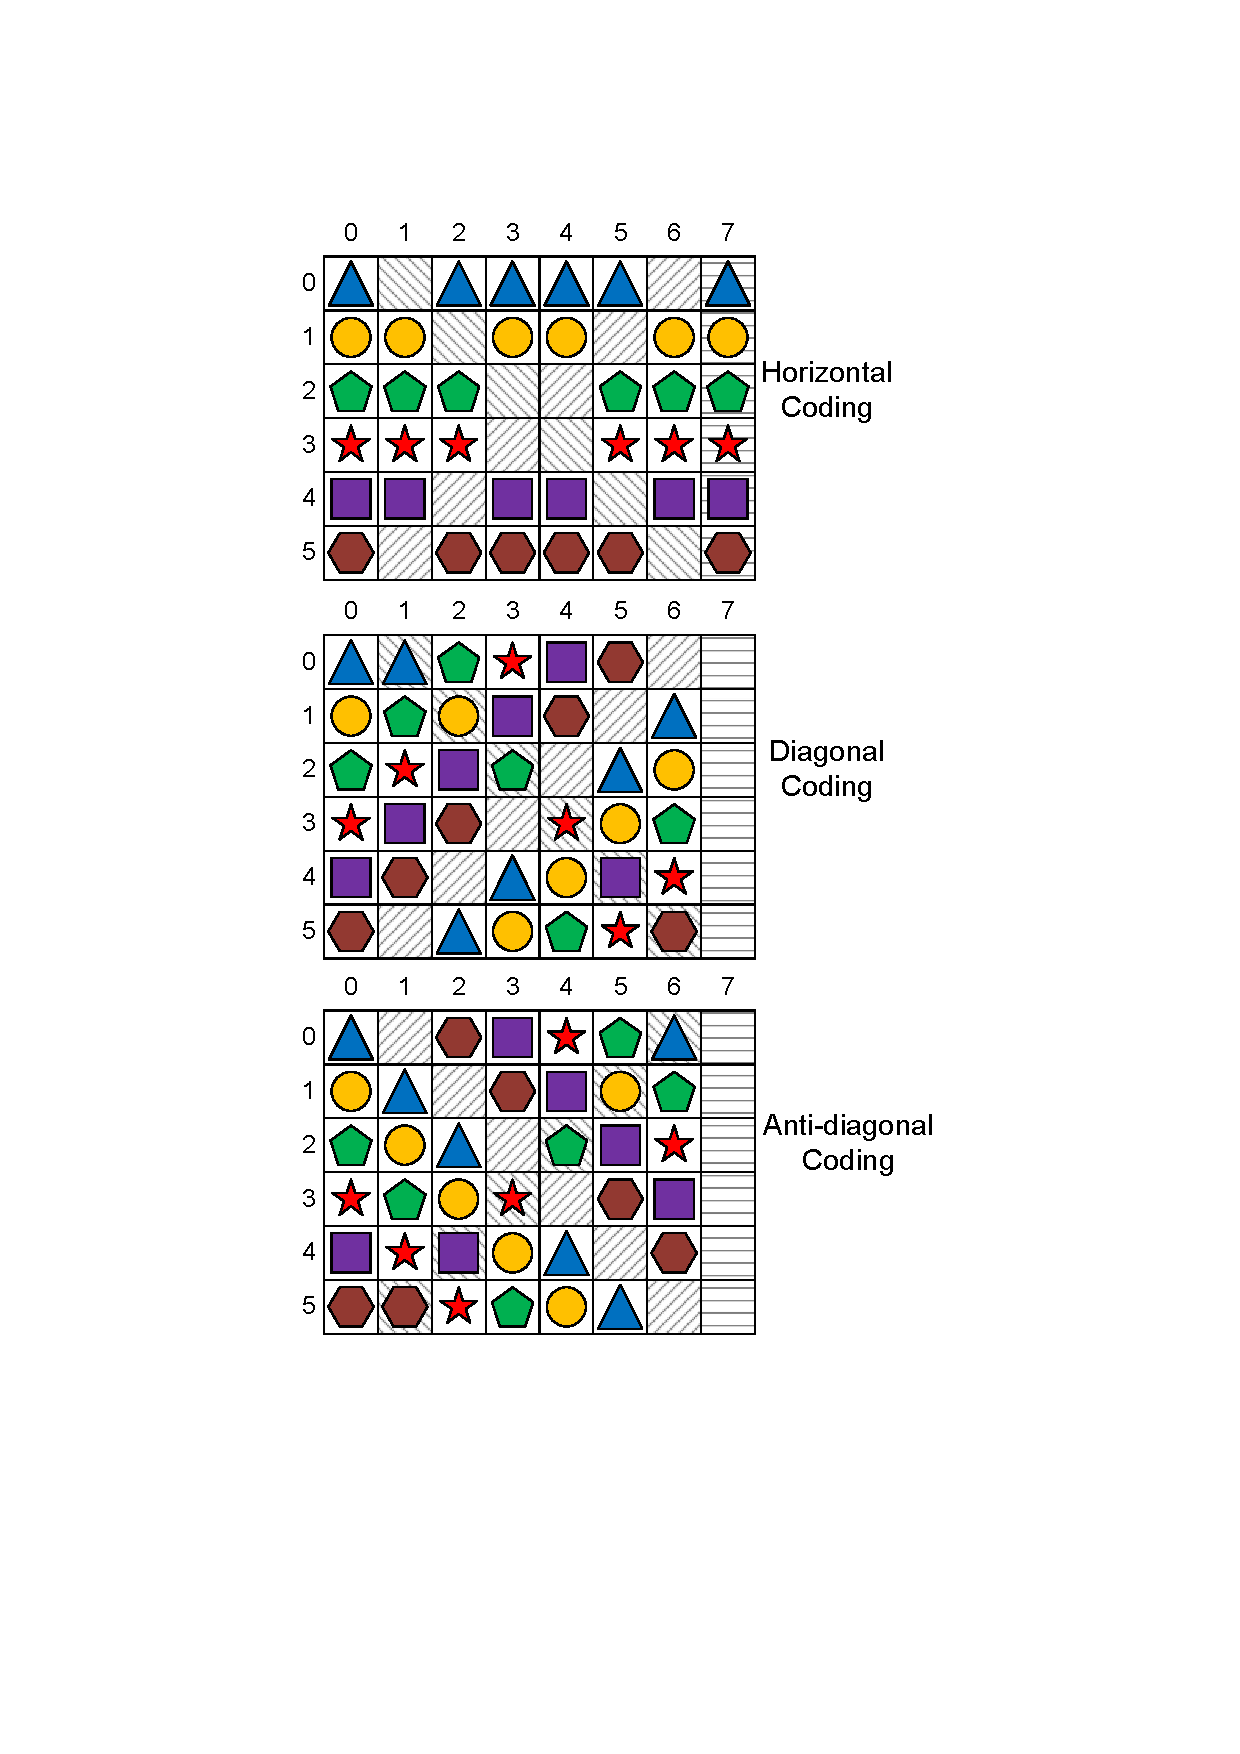
\includegraphics[height=6cm]{photo/TIP.pdf}\label{fig-tip}
}\vspace{-3mm}
\caption{Encoding of STAR (Figure \ref{fig-star}) and TIP (Figure \ref{fig-tip}) code ($p = 5$). Each column represents a node, each block represents an element, and parity chains are represented by elements with same shape. STAR requires the number of data nodes to be $p$, and TIP requires that to be $p-2$, where $p$ is a prime number.}
\vspace{-3mm}
\label{fig-star-tip}
\end{figure}

TIP-Code is also an XOR-based 3DFTs erasure code.
Compared with STAR code, the parities are generated independently, which reduces the number of I/O operations for partial stripe writes.

\subsection{Approximate Storage}
Approximate storage is an innovative approach for storage devices \cite{zhao2017approximate, sampson2014approximate, guo2016high, jevdjic2017approximate}, which enable applications to store data approximately. It can improve the performance, lifetime, or reduce the power consumption of different storage devices.

Specifically, for video applications, there are several approximate storage methods \cite{guo2016high, jevdjic2017approximate} for bit-level reliability in progressively encoded multimedia data.  \cite{guo2016high} identifies the relative importance of the encoded bits on the image quality and apply different levels of error correction. \cite{jevdjic2017approximate} shows how reliability of video storage can be traded for density and achieves the optimal quality/density points by tracking visual and metadata dependencies within the encoded bit stream.


\begin{table}[ht]\footnotesize
\centering
\caption{
Comparison of storage overhead, fault tolerance and computing overhead among various storage methods for video files}\label{tab-AS-EC-AP}
\begin{tabular}{|p{2cm}<{\centering}|p{1.2cm}<{\centering}|p{1cm}<{\centering}|p{1.1cm}<{\centering}|p{1.1cm}<{\centering}|}
\hline
Schemes & Storage Overhead & Fault Tolerance & Computing Overhead & Layer \\ \hline
Data Compression & low & / & high & \begin{tabular}[c]{@{}c@{}}Application\\Level\end{tabular} \\ \hline
RS-based EC for 3DFTs & high & high & high & \multirow{6}{*}{\begin{tabular}[c]{@{}c@{}}Device\\Level\end{tabular}}\\ \cline{1-4} 
XOR-based EC for 3DFTs & high & high & low & \\ \cline{1-4} 
RAID-6 & low & low & low & \\ \cline{1-4} 
RAID-5 & medium & medium & low & \\ \cline{1-4} 
Approximate Storage & very low & very low & low & \\ \cline{1-4} 
Approximate Code & low & high & low & \\ \hline
\end{tabular}
\end{table}

\subsection{Our Motivation}
We summarize various methods to reduce storage cost for video files in Table \ref{tab-AS-EC-AP}, the device level scheme of existing 3DFTs has high storage overhead, while RAID-5 or RAID-6 maintains medium storage overhead but sacrifice fault tolerance. Although approximate storage achieves low cost, its reliability cannot be satisfied in cloud environment. Application layer methods such as compression algorithms have high computational overhead and need to be used together with erasure codes to ensure reliability.
Therefore, the existing solution cannot guarantee high reliability and low overhead at the same time of video storage.

From the summary of Table \ref{tab-AS-EC-AP}, existing solutions have their drawbacks on providing high reliability with low storage cost. 
A feasible solution is combining various erasure codes with tiered storage \cite{krish2014hats} \cite{wang2014balancing} \cite{zhang2010automated} \cite{udipi2012lot}, which motivates us to propose Approximate Code.

\begin{figure*}[ht!]
\centering
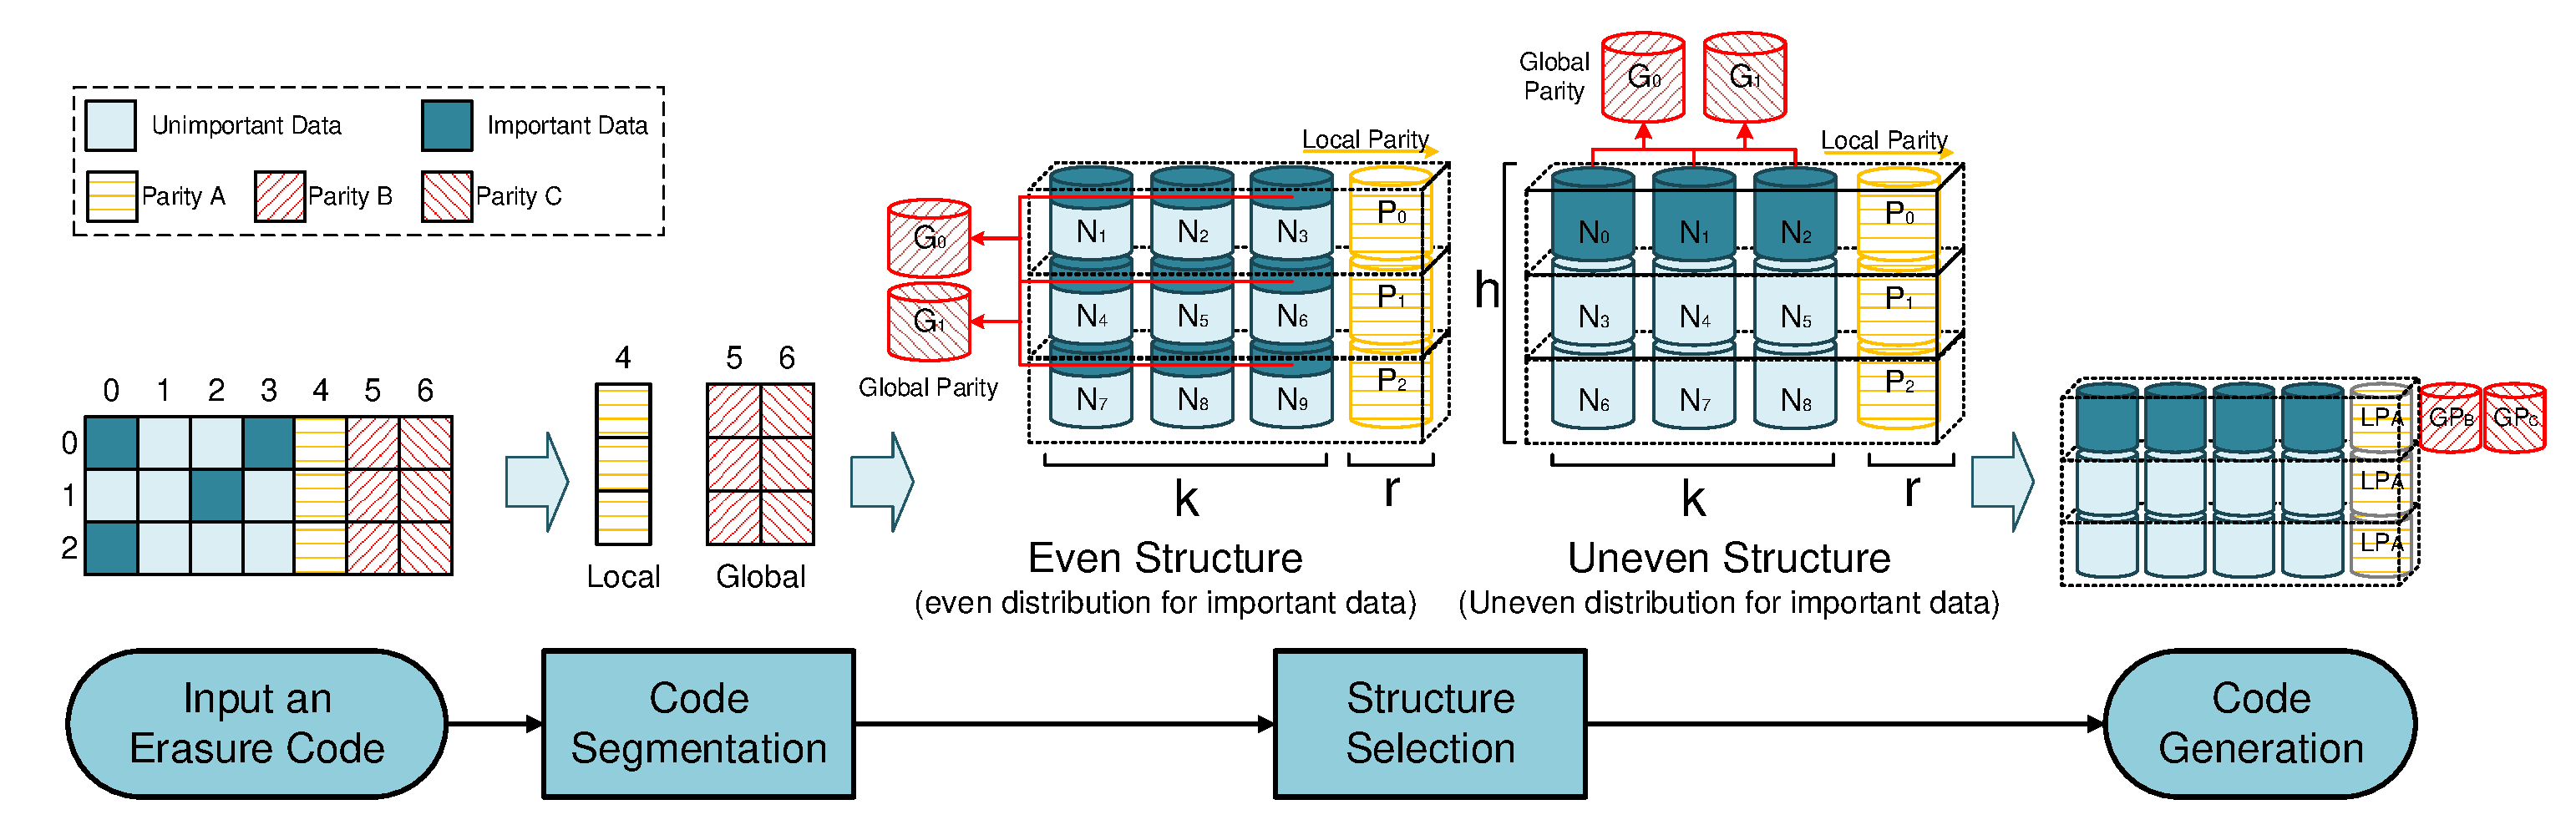
\includegraphics[width=0.95\linewidth]{photo/Framework-v3.pdf}
\caption{The framework of Approximate Code}
\label{fig-framework}
\end{figure*}

\section{Approximate Code}\label{ApCode}
In this section, we introduce the Approximate Code Framework and its properties through a few simple examples.

\subsection{Overview of Approximate Code Framework}
The Approximate Code framework contains four main steps, code input, code segementation, structure selection and code generation, as shown in Figure \ref{fig-framework}.

\subsubsection{Code Input}
Acquire an erasure coding input and get the corresponding parameters. Typically, for cloud storage systems, erasure codes used in 3DFTs are accepted as the input. Several parameters related to erasure codes need to be collected, such as the number of data nodes $k$ and the number of parity nodes $r$.

\subsubsection{Code Segmentation}
For an inputted erasure code, we assume that its fault tolerance is $x$. The Approximate Code first splits its parities into two parts, local and global parities. The local parities are used for all data, while the global parities focus on the important data. Code segmentation are designed to ensure that local parities can tolerate any $r$ node failures, so the fault tolerance of unimportant data is $r$. For important data, the code segmentation ensures that the important data have the capabilities of fault tolerance by up to $x$ nodes.

For example, several erasure codes in 3DFTs like STAR have three types of parities, horizontal, diagonal and anti-diagonal parities. In the code segmentation step, the horizontal parities are regarded as local parities, which are separated from the diagonal/anti-diagonal parities (shown in Fig. \ref{fig-appr-star} and illustrated in \ref{APPRXOR} in detail).

\subsubsection{Structure Selection}
The framework choose the structure after code segmentation.
There are two main structures that distribute important and unimportant data in different ways.
As shown in Figure \ref{fig-framework}, in Even structure, important data are distributed uniformly among all data nodes. The other structure is Uneven structure, which stores the important data among several nodes dedicatedly.
%We specify that in Even structure, the ratio of important data to each node is $1/h$, thereby ensuring that the number of important data in both Even structure and Uneven structure just fills up $k$ nodes.

Since Even structure distributes important data across each node, it guarantees a balanced workload. Uneven structure concentrates important data into several dedicated nodes, and provides better reliability based on failure locality. \textcolor{red}{[CITE FAILURE MODEL]}.

\subsubsection{Code Generation}\label{code-gen}
After code segmentation and structure selection, the Approximate Code Framework generates an approximate form of the inputted erasure code.
The construction of the Approximate Code is determined by 4 parameters $k$, $r$, $g$, $h$ and the structure type.

We define the output Approximate Code as \textbf{APPR.CodeName ($k,r,g,h$, Structure Type)}, where ``CodeName'' is the name of the input erasure code. Structure type is Even or Uneven and the default configuration selects both two structures.

According to these parameters, Approximate Code framework divides the data/parity nodes into several local stripes. Each local stripe has $n$ nodes,  
In a $n$-node stripe, $k$ of them are data nodes and $r=n-k$ nodes are local parity nodes.
Assume the ratio of important data is $1/h$, the framework utilizes $h$ local stripes to construct a global stripe, which includes $k*h$ data nodes and $r*h$ local parity nodes in total.
In a global stripe, $g$ additional nodes are designed for global parities, which are calculated by the important data, so the total number of nodes $N$ in APPR.CodeName ($k,r,g,h$) is
$N= h*(k+r) + g$.

Approximate Code guarantees that the unimportant data can tolerate any $r$ node failures and the important data can tolerate any $r+g$ node failures.
Since the 3DFTs is a typical configuration, we mainly discuss the situation of $r+g=3$ in the rest of our paper, so $r$ is usually $1$ or $2$.%, except section \ref{appr-rsbased}.

\subsection{Approximate RS-based Codes}\label{appr-rsbased}
The operation of RS($k,m$) is based on the GF, which provides $m$ independent horizontal parities for $k$ data nodes. Therefore, the code segmentation for RS is arbitrary, that is, it supports any $r=p-g(0<g<m)$. RS also supports both two structures. We then introduce the construction of Approximate RS Code and Approximate LRC.

\subsubsection{Approximate RS Code}
We consider the inputted erasure code as RS($4,3$), as shown in Figure \ref{fig-RS-2}. Three horizontal parities are divided into one local and two global parities with the Uneven structure and it generate Approximate RS Code ($4,1,2,3$,Uneven).
As a result, the unimportant data and their corresponding parities constitutes a RS ($4,1$) array, and the important data and their corresponding parities form a RS($4,3$).

\subsubsection{Approximate LRC}

\begin{figure}
    \centering
    \subfigure[The generation of APPR.RS Code]{
        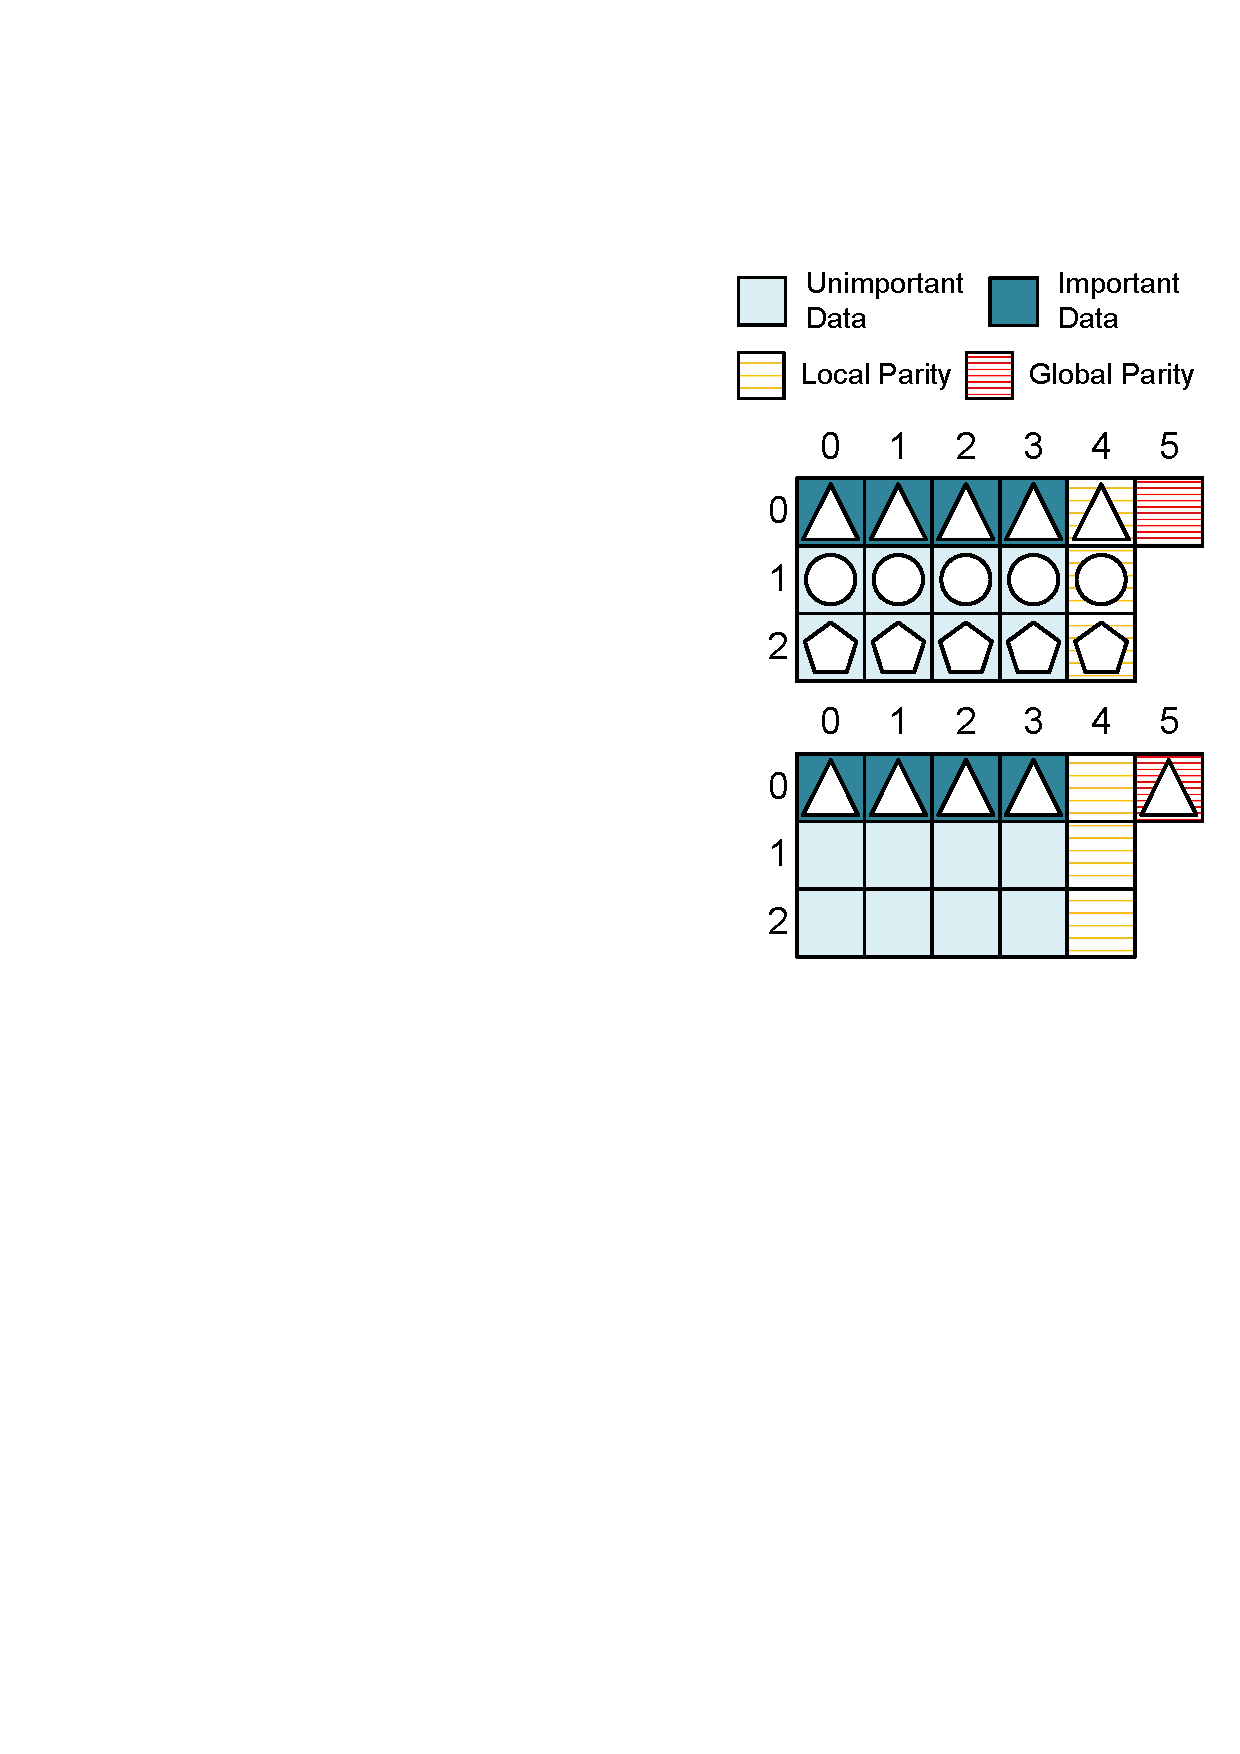
\includegraphics[width=0.8\linewidth]{photo/RS-2.pdf}\label{fig-RS-2}
    }

    \subfigure[The generation of APPR.LRC]{
        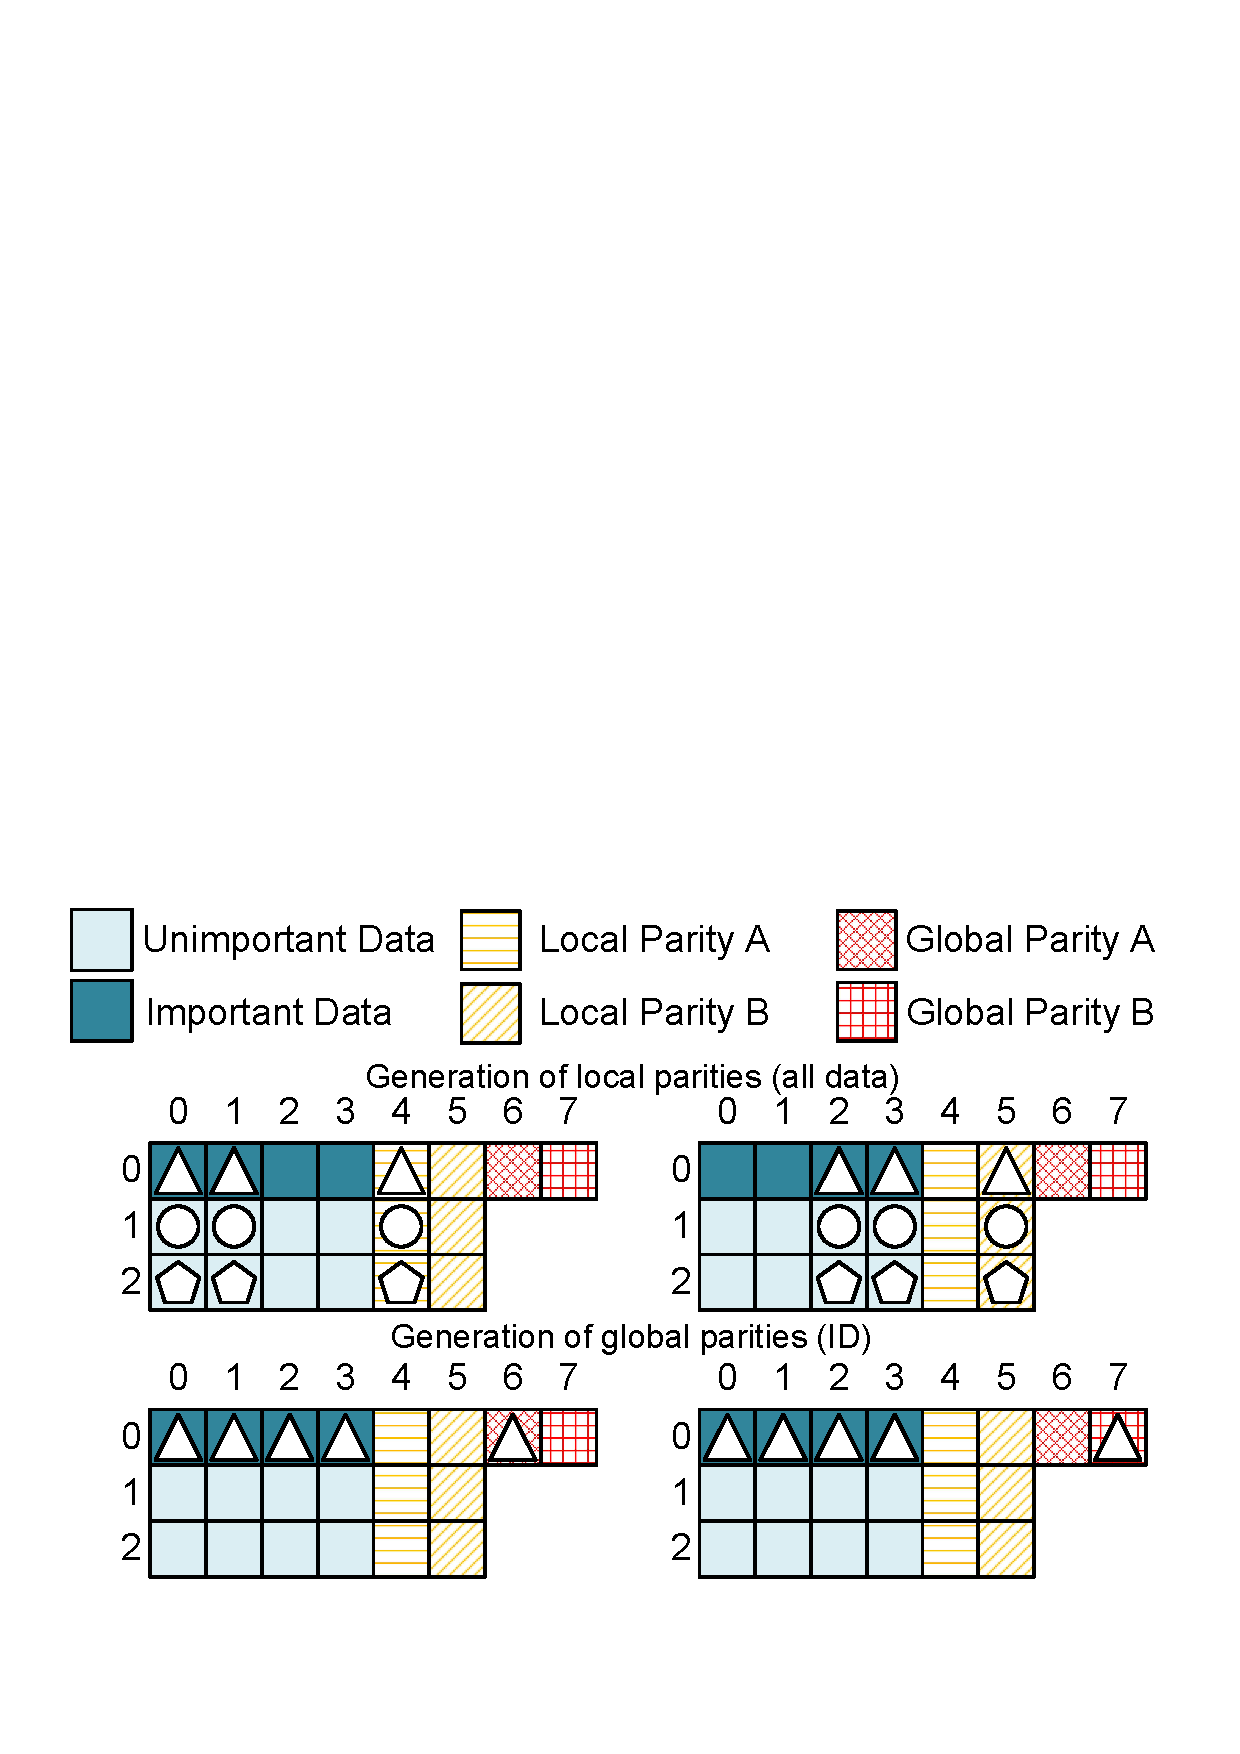
\includegraphics[width=0.8\linewidth]{photo/LRC-2.pdf}\label{fig-LRC-2}
    }
    \caption{The construction and the encoding process of APPR.RS ($4,1,2,3$)}
\end{figure}

\subsection{Approximate XOR-based Codes}\label{APPRXOR}
Since we mainly provide 3DFTs for important data, we prefer to construct Approximate Code with several XOR-based codes to provide faster encoding and reconstruction speed than RS-based codes. Here we introduce two typical construction of Approximate XOR-based codes, Approximate STAR Code and Approximate TIP-Code.

\begin{figure}[ht]
\centering
\subfigure[Structure selection of APPR.STAR Code]{
    \label{fig-ap-tip-str}
    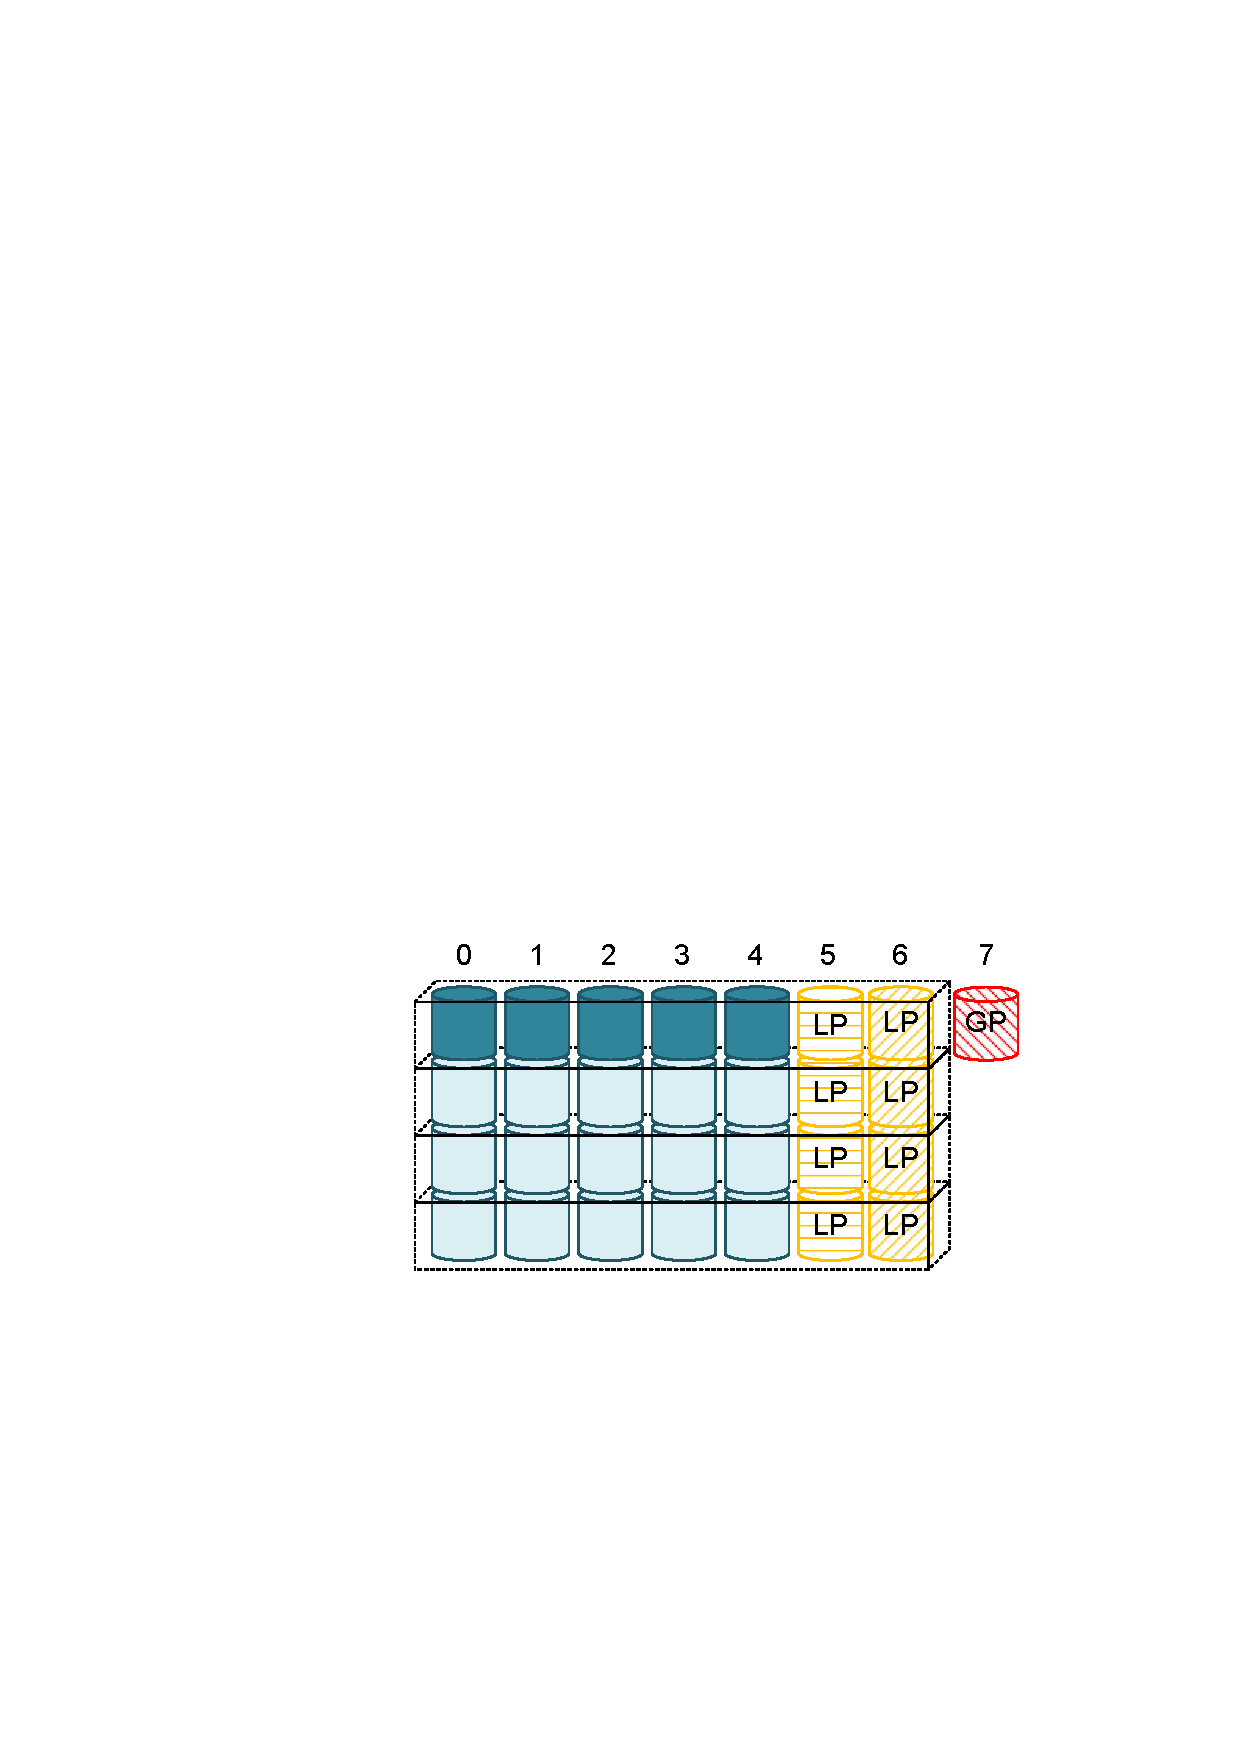
\includegraphics[width = 0.5\linewidth]{photo/APPR-STAR-STR.pdf}
}

\subfigure[Generation process]{
    \label{fig-ap-tip-GEN}
    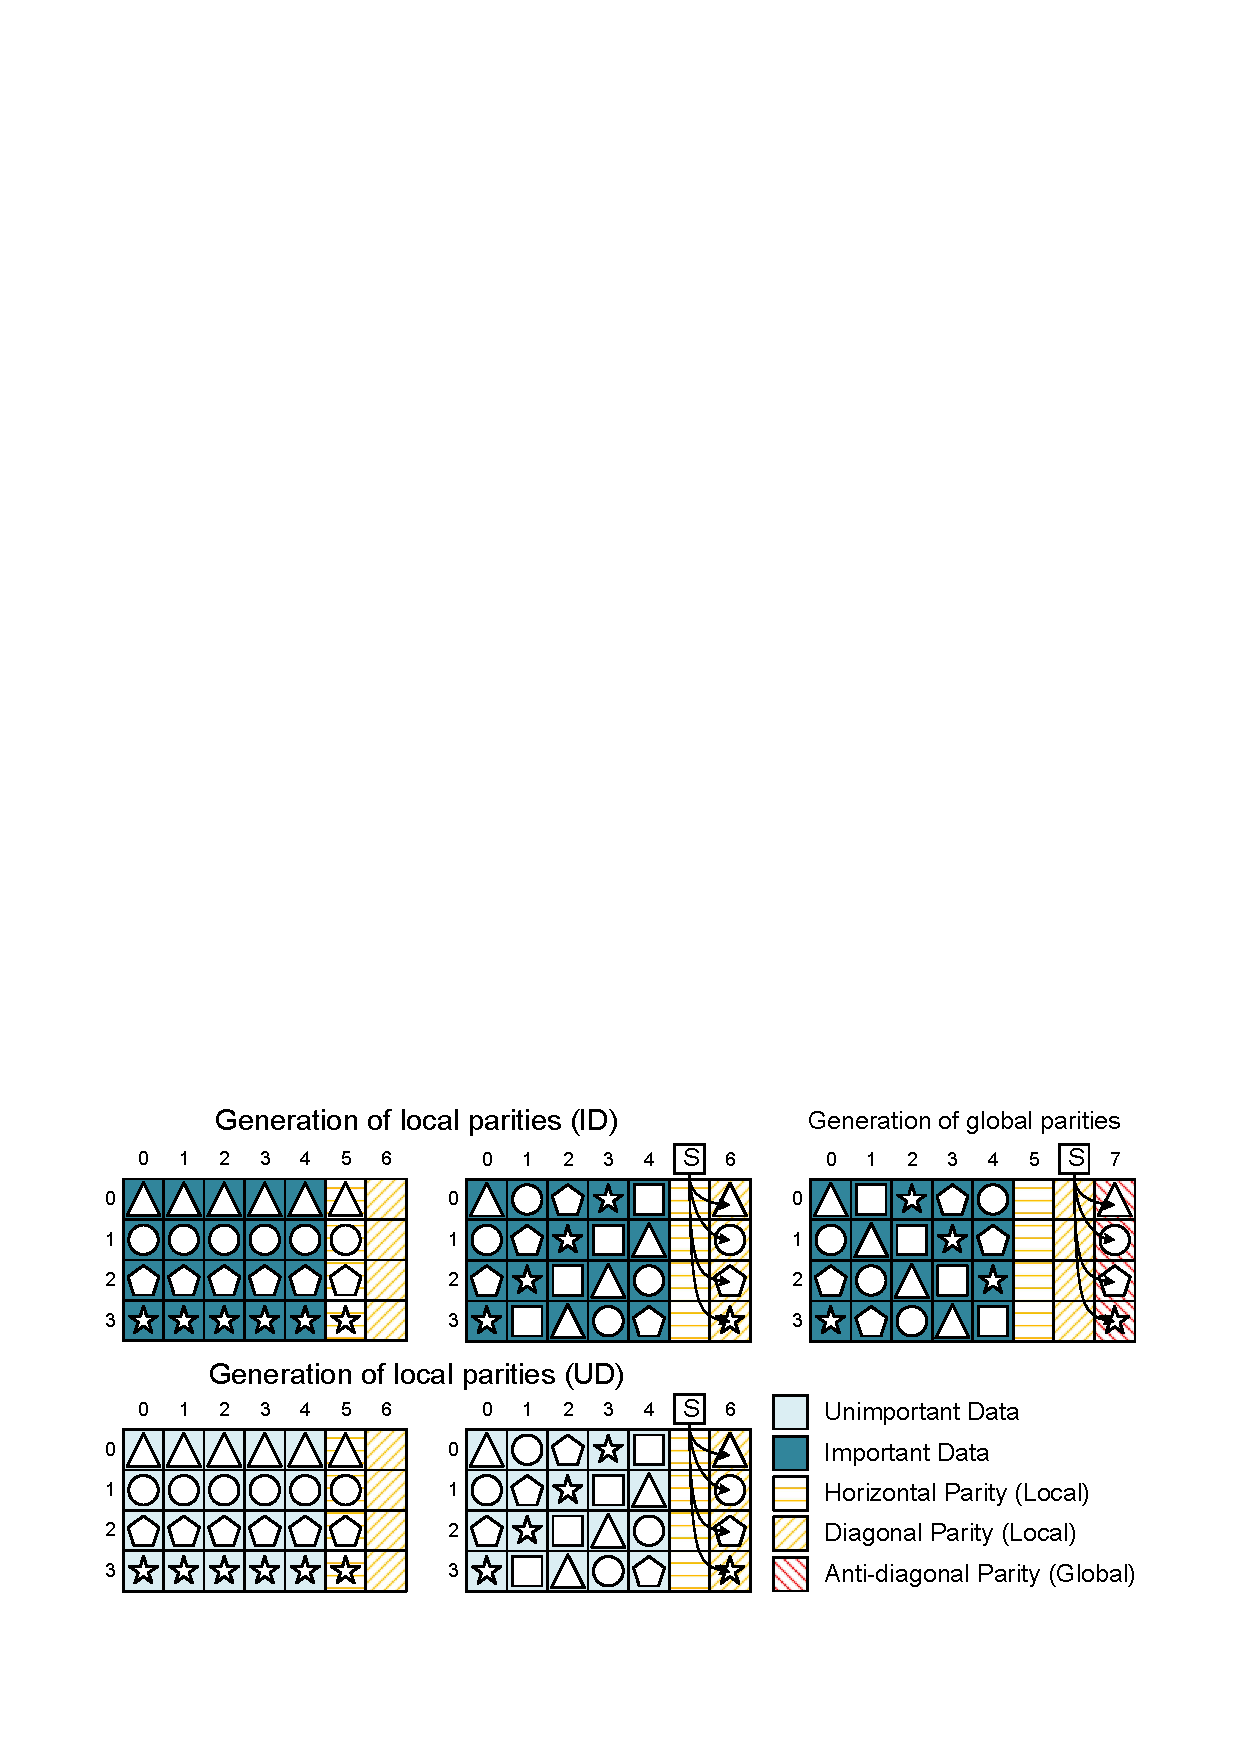
\includegraphics[width = \linewidth]{photo/APPR-STAR-GEN.pdf}
}
\caption{The construction and the encoding process of APPR.STAR ($5,2,1,4$,Uneven)}
\label{fig-appr-star}
\end{figure}


\subsubsection{Approximate STAR Code}
Figure \ref{fig-appr-star} shows the construction and the encoding process of APPR.STAR($5,2,1,4$,Uneven).
As introduced in \ref{existEC}, STAR Code \cite{STAR} has 3 parity chunks and it is a tipical 3DFTs XOR-based erasure code.
Since STAR is a direct extension of EVENODD\cite{EVENODD}, that is to say, STAR code that removes the anti-diagonal parity is the typical RAID-6 code EVENODD. As shown in Figure \ref{fig-appr-star}, in this case, the horizontal and diagonal parity are used as local parities while the anti-diagonal parity is defined as global parity.
According to the construction requirements of STAR, each node is divided into 4 blocks.

Briefly, APPR.STAR($5,2,1,4$,Uneven) can be considered to be important data encoded by the full STAR, while the unimportant data is encoded by a portion of STAR, EVENODD. It is plain to see that important data can tolerate any 3 node failures while unimportant data can tolerate any 2 node failures.

\subsubsection{Approximate TIP-Code}

\begin{figure}[ht]
\centering
\subfigure[Structure selection of APPR.TIP-Code]{
    \label{fig-ap-tip-str}
    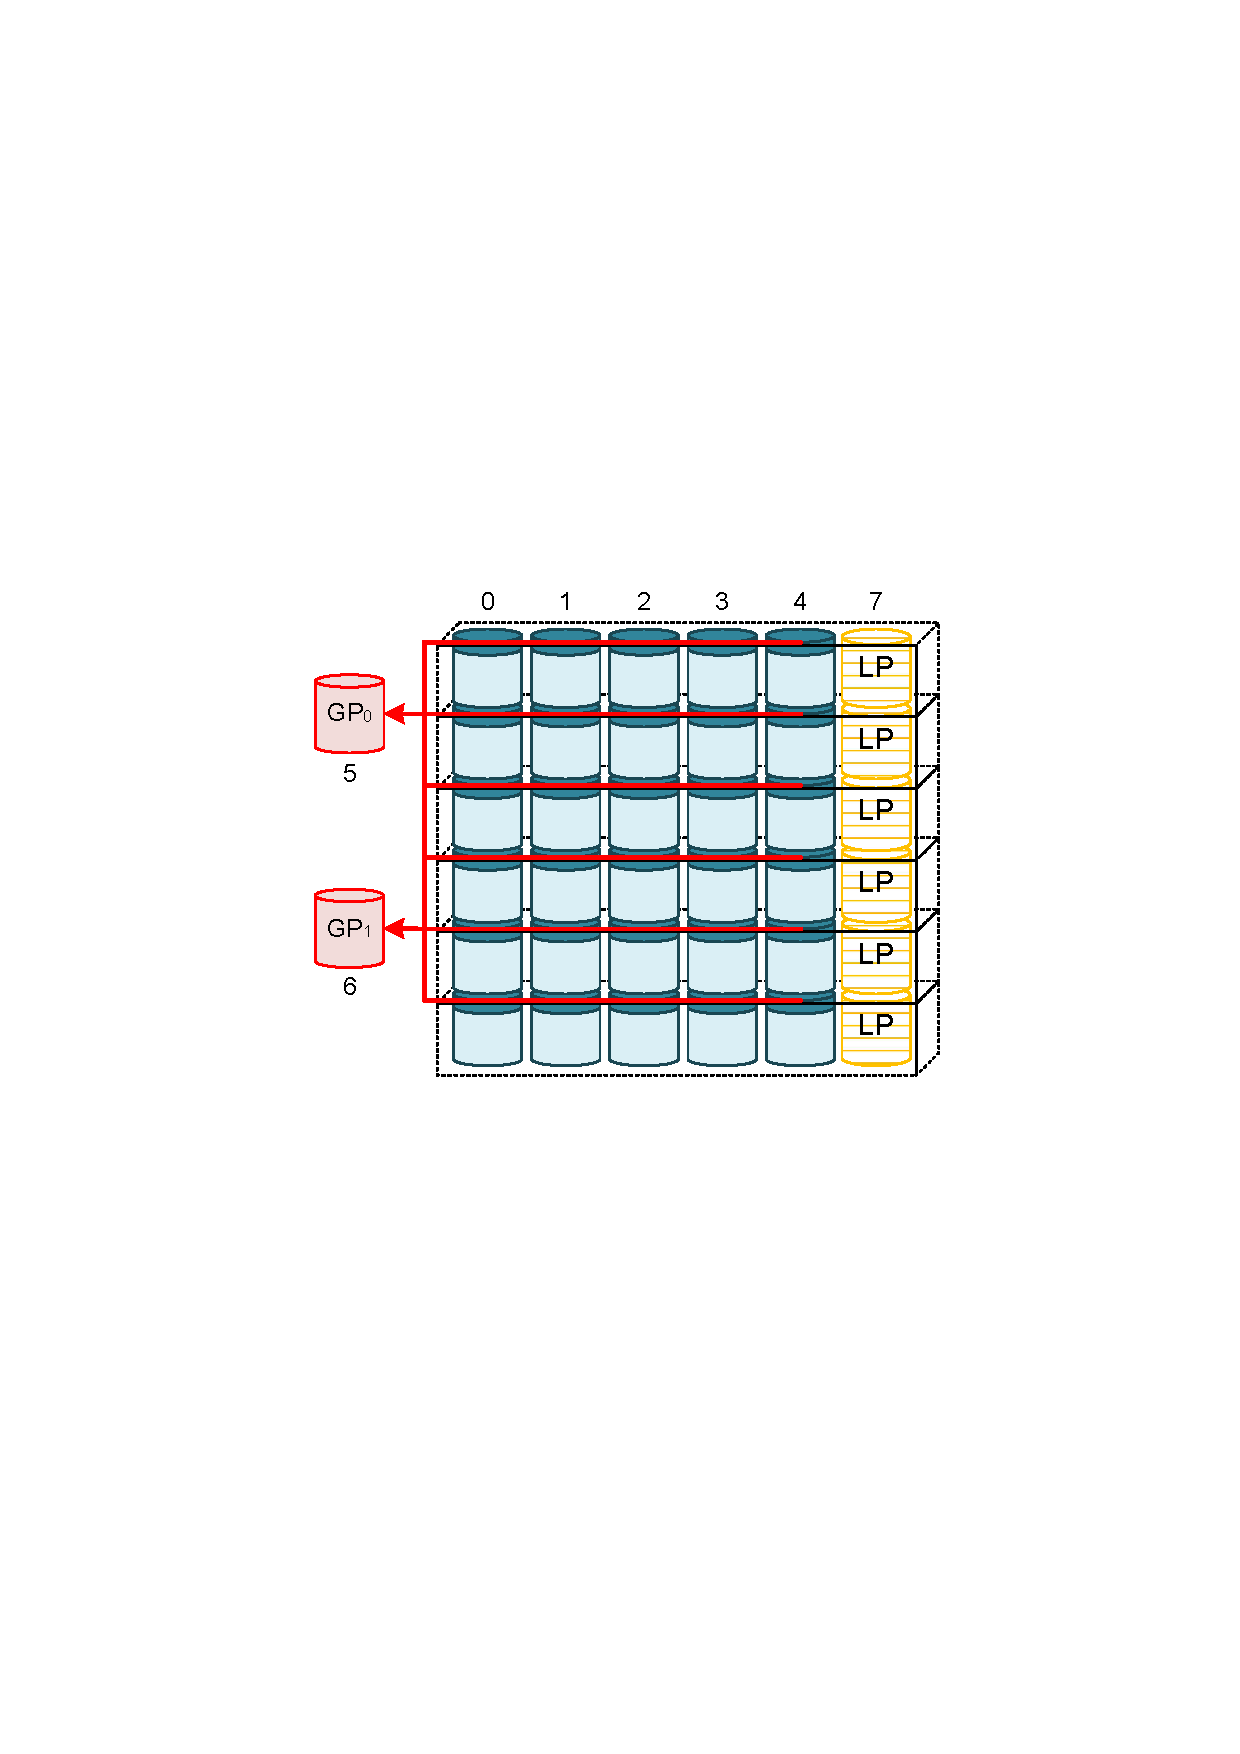
\includegraphics[width = 0.45\linewidth]{photo/APPR-TIP-STR.pdf}
}
\hspace{2pt}
\subfigure[Generation of local parities]{
    \label{fig-ap-tip-lP}
    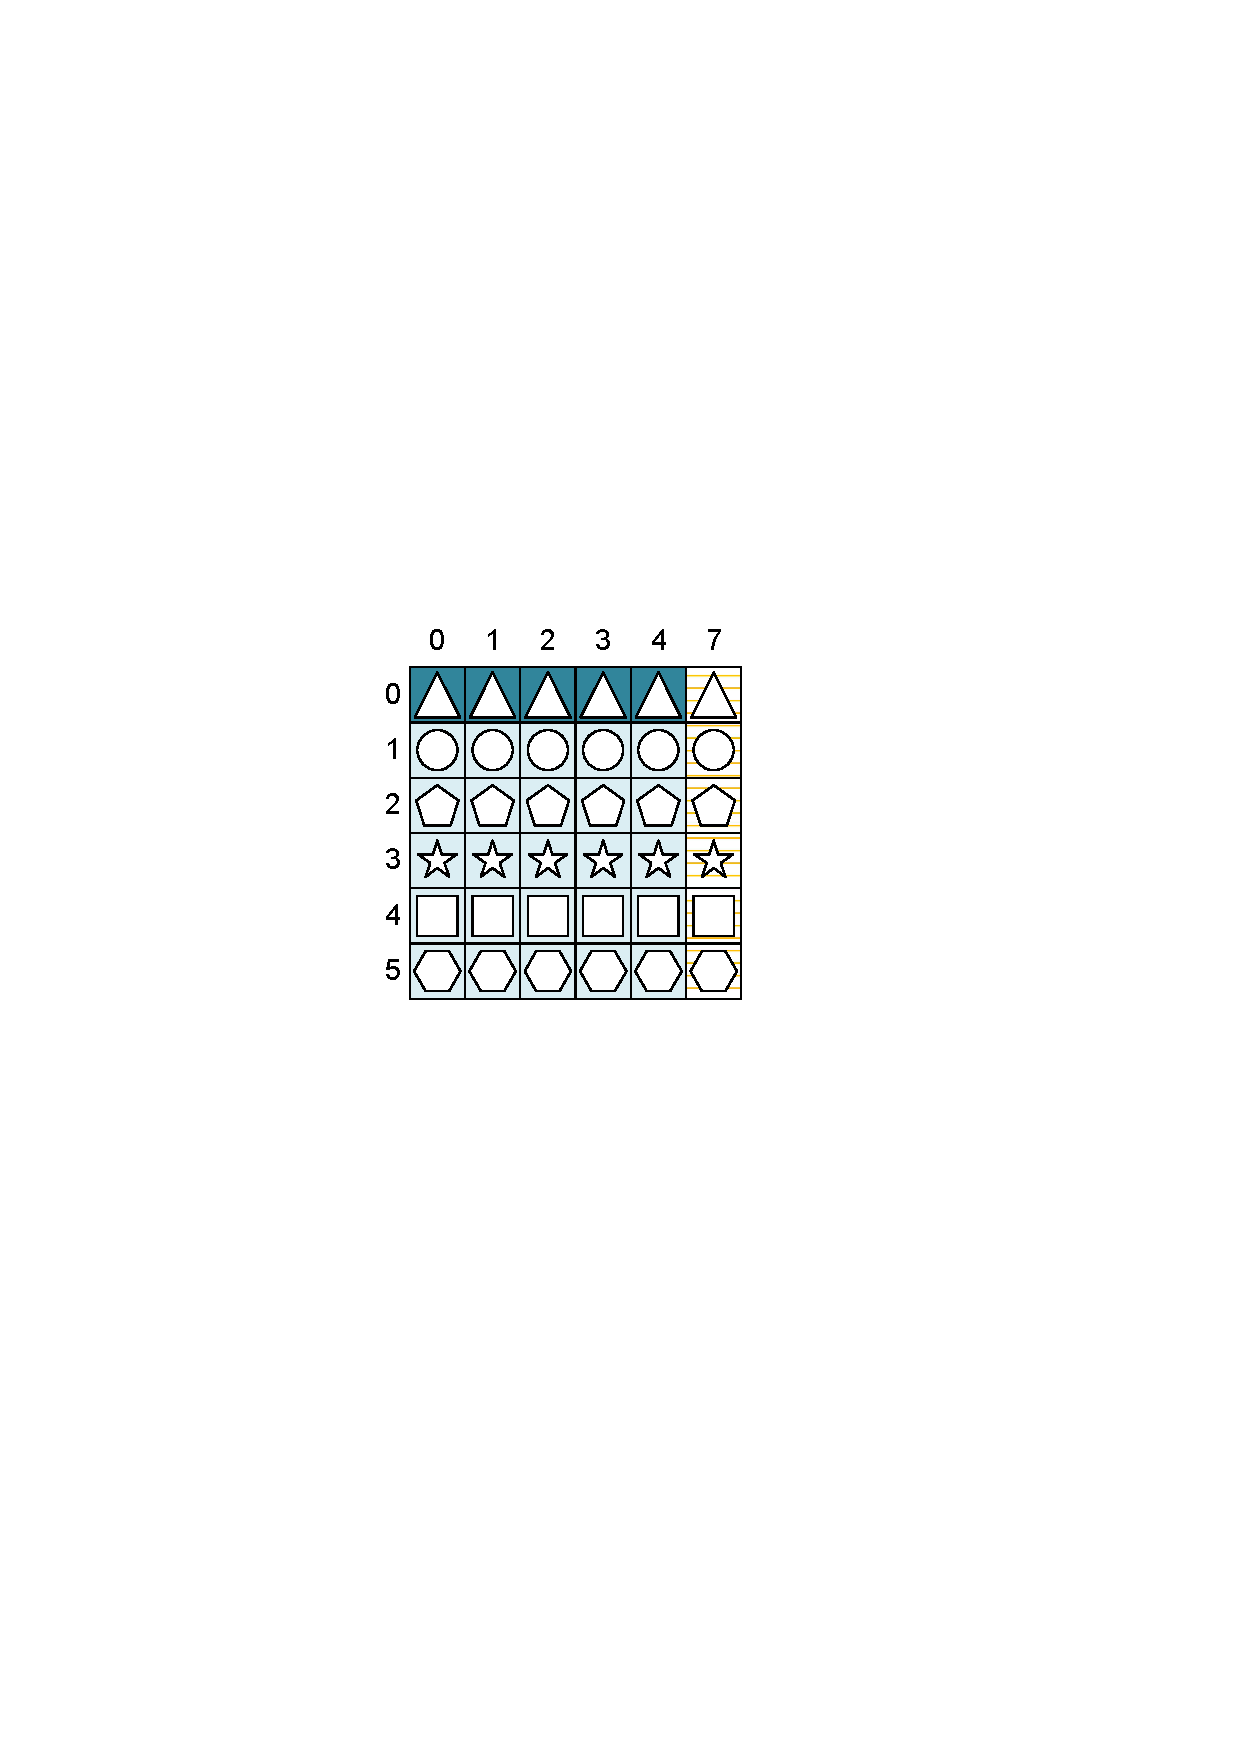
\includegraphics[width = 0.3\linewidth]{photo/APPR-TIP-LO.pdf}
}

\subfigure[Generation of global parities]{
    \label{fig-ap-tip-GP}
    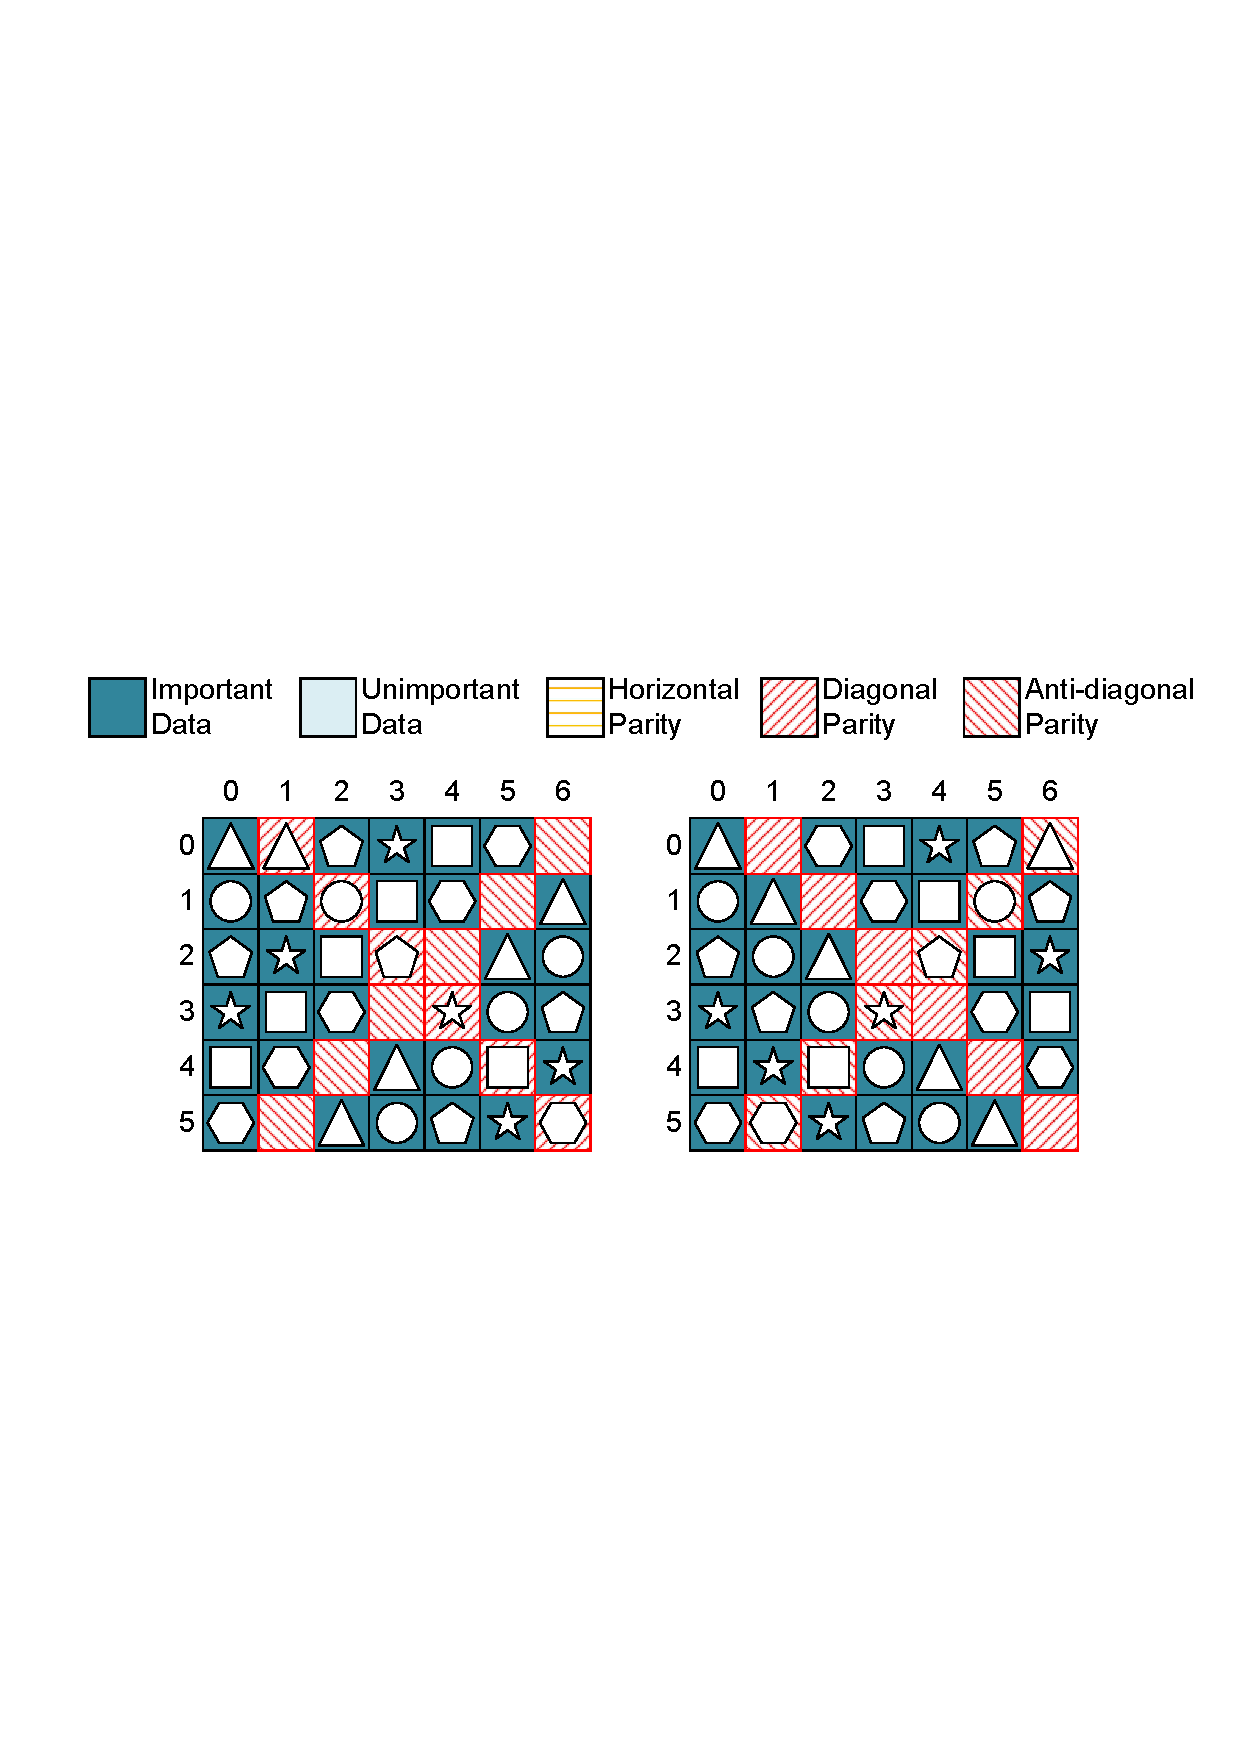
\includegraphics[width = 0.8\linewidth]{photo/APPR-TIP-GL-v2.pdf}
}
\caption{The construction and the encoding process of APPR.TIP ($5,1,2,6$,Even). The node 5 and 6 in TIP-Code is defined as the global parity nodes in this case.}
\label{fig-ap-TIP}
\end{figure}

We then introduce the generation of APPR.TIP($5,1,2,6$,Even).

In the code segmentation phase, we split TIP-Code into horizontal, diagonal and anti-diagonal parity. The important data is arranged in Even structure. However, since the parity block of the TIP is distributed over a series of nodes, the code generation process is different from that of the STAR.

We first generate local parity nodes by the horizontal parity for the important and unimportant data in each node. Then, we arrange the important data blocks as the type of Figure \ref{fig-tip-1}.
We use diagonal and anti-diagonal parity to encode the important data and define the last 2 node (Node 5 and 6) as the global parity nodes.

As shown in Figure \ref{fig-ap-TIP}, 30 data nodes form 6 stripes, where important data accounting for 1/6 of each node.
All data nodes generate 6 local parity nodes.
Important data blocks are rearranged to fit the parity form of TIP-Code and generate two global parity nodes.

\subsection{Reconstruction Process and Fault Tolerance}\label{ReconstructionFT}
When $r$ or less nodes fail, all the data can be reconstructed by local parities.
When $r+g$ or less nodes fail, all the important data can be reconstructed by local and global parities.

However, in most cases, the loss of more nodes is also recoverable. We only consider two situations: $r+1$ and $r+g+1$.
The former exceeds the fault tolerance of unimportant data so we calculate the $P_{U}$, while the latter exceeds the fault tolerance of important data and we calculate the $P_{I}$.
As mentioned in Section\ref{code-gen}, $r+g$ is set to 3.

We exhaust all the conditions that may cause data loss and calculate the corresponding probability to calculate $P_{I}$ and $P_{U}$.
Approximate Codes based on different structures also have different fault tolerance and reconstruction cases, so we discuss Even structure and Uneven structure respectively.

\subsubsection{Lost $r+1$ nodes}
Under Even structure, the unimportant data nodes are recoverable as long as the node loss per stripe does not exceed $r$ and the global parity nodes do not need to be considered.
There are $\binom{N}{r+1}$ cases of loss of $r+1$ nodes and $h$ stripes in all. In each stripe, $\binom{k+r}{r+1}$ cases will result in unrecoverable of data.

Under Uneven structure, only $h-1$ stripes contain unimportant data, so $P_{U}$ is
\begin{align}
    P_{U-Even} &= 1 - \frac{h \times \binom{k+r}{r+1}}{\binom{N}{r+1}}\\
    P_{U-Uneven} &= 1 - \frac{(h-1) \times \binom{k+r}{r+1}}{\binom{N}{r+1}}
\end{align}

\subsubsection{Lost $4$ nodes}
The number of all 4-node lost cases is $\binom{N}{4}$.
We calculate the total number of cases in which all important data may be lost based on the different losses of the global parity nodes. The results are as follows:
\begin{align}
    P_{I-Even} = 1 - h*&\frac{\sum_{i=0}^{g} {\binom{k+r}{4-i}*\binom{g}{i}} }{\binom{N}{4}}  (g=1,2)\\
    P_{I-Uneven} &= 1 - \frac{\binom{k+3}{4}}{\binom{N}{4}}
\end{align}

According to the equations above, in Approximate RS ($3,1,2,3$, Even), $80.21\%$ 2-node failure cases are recoverable for unimportant data nodes, and $95.50\%$ 4-node failure is recoverable for important data nodes. In Approximate RS ($3,1,2,3$, Uneven), $P_U=86.81\%$ $P_{I}=98.50\%$.


\subsection{Properties of Approximate Code}\label{properties}

We analyze the nature of the Approximate Code from the following aspects, and the calculation method of the relevant indicators is given in Table \ref{tab-properties}.
\begin{itemize}
    \item Low Storage Overhead: Approximate Code reduces storage overhead by approximating and tiered storage strategies. This property is more pronounced for data with a smaller proportion of important data.
    \item Optimal Update Complexity: When one node is updated, Approximate RS Code only needs to write $r$ local parity nodes and only $g/h$ global parity nodes on average besides the write of data node.
    \item High reliability for important data. The Approximate Code guarantees 3DFTs for important data.
    \item Flexibility. The implementation of the Approximate Code can be based on any erasure codes in 3DFTs.
\end{itemize}

\begin{table}[htb]
\centering
\caption{Comparison of storage overhead, fault tolerance and average single write performance between RS, LRC, STAR, TIP, Approximate RS, Approximate STAR and Approximate TIP, where $p$ is a prime number.}\label{tab-properties}
\begin{tabular}{|c|c|c|c|}
\hline
EC & \begin{tabular}[c]{@{}c@{}}Storage\\ Overhead\end{tabular} & \begin{tabular}[c]{@{}c@{}}Fault\\ Tolerance\end{tabular} & \begin{tabular}[c]{@{}c@{}}Ave Single Write\\ Overhead \end{tabular} \\ \hline
RS($k,r$) & $(k+r)/k$ & $r$ & $r+1$ \\ \hline
LRC($k,l,r$) & $1+(l+r)/k$ & $r+1$ & $r+2$ \\ \hline
STAR($p$) & $(p+3)/p$ & $3$ & $6-\frac{4}{p}$ \\ \hline
TIP-code($p$) & $\frac{p+1}{P-2}$ & $3$ & 4 \\ \hline
\begin{tabular}[c]{@{}c@{}}APPR.RS\\ ($k,r,g,h$)\end{tabular} & \multirow{3}{*}{$\frac{(k+r)h+g}{kh}$} & $r+g$ & $1+r+\frac{g}{h}$ \\ \cline{1-1} \cline{3-4}
\begin{tabular}[c]{@{}c@{}}APPR.STAR\\ ($k,2,1,h$)\end{tabular} &  & 3 & $2\frac{k-h-1}{kh}+4$ \\ \cline{1-1} \cline{3-4}
\begin{tabular}[c]{@{}c@{}}APPR.TIP\\ ($k,1,2,h$)\end{tabular} &  & 3 & $2+\frac{2}{h}$ \\ \hline
\end{tabular}
\end{table}

\subsection{Implementation}\label{Implementation}
\begin{figure}[htb]
\centering
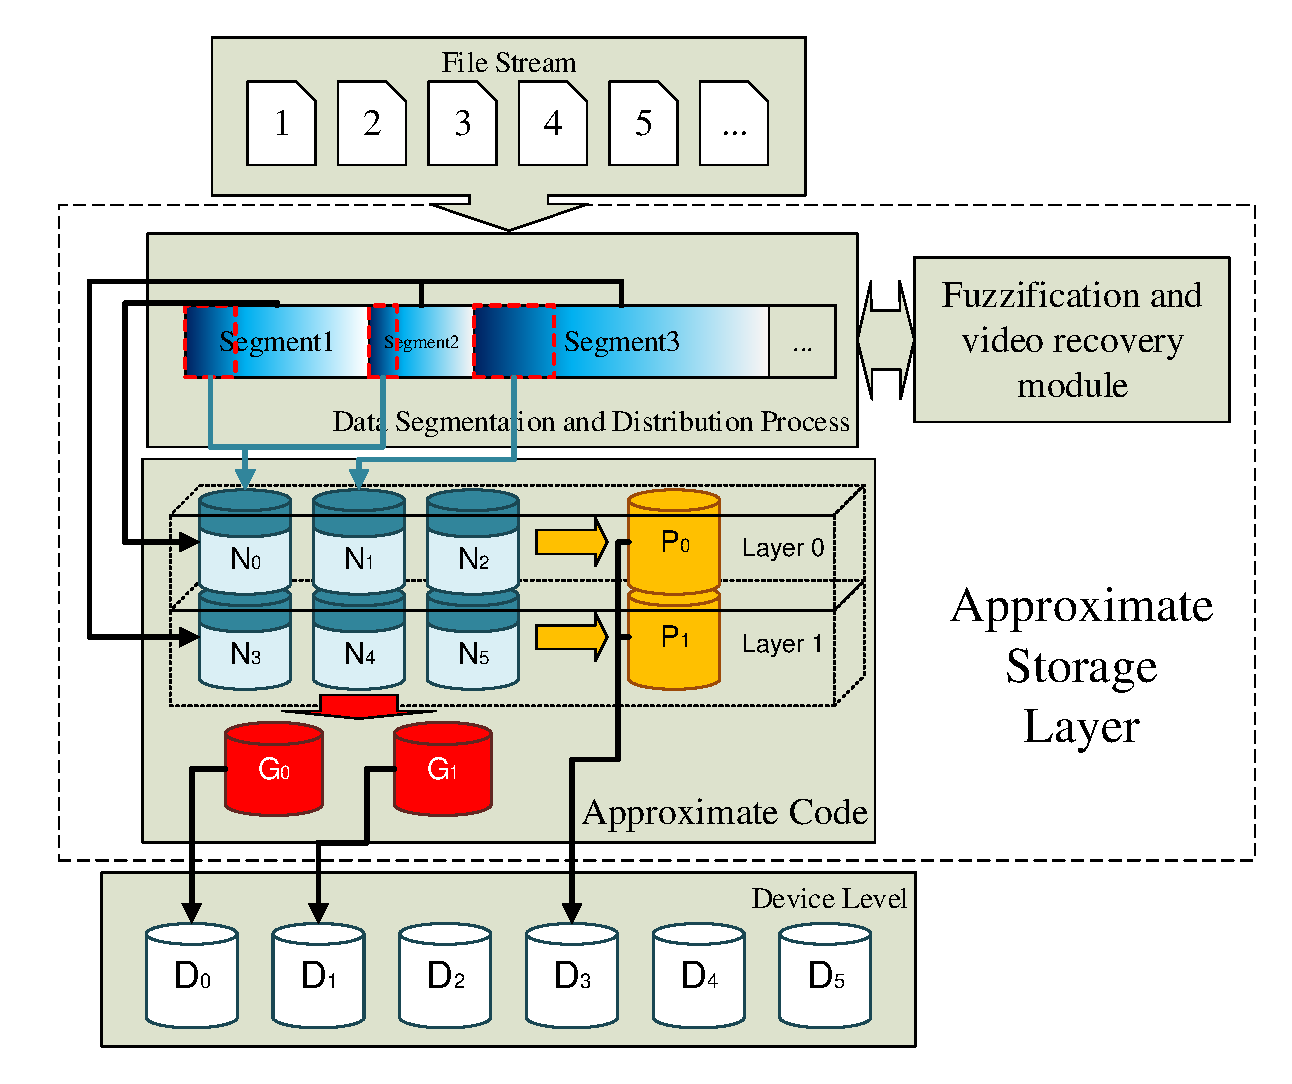
\includegraphics[width=0.8\linewidth]{photo/implementation-V2.pdf}
\caption{Overview of Approximate Storage Layer}
\label{fig-implementation}
\end{figure}

Compared with the traditional scheme that does not consider the meaning of the upper layer data, the Approximate Code pays attention to the difference of the importance of the data, so an intermediate layer between the upper layer application and the underlying distributed storage system is necessary. We call it the approximate storage layer, which include 3 parts: data identification and allocation, encoding and decoding process of Approximate Code and the video fuzzification and recovery.

\subsubsection{Data Segmentation and Distribution module}
The data segmentation module splits the video file stream into multiple data segments and automatically discriminates the important data. A natural approach is to follow the GOP segmentation. According to the \ref{video storage}, the GOP of the encoded video starts with an I frame, and all the data in that GOP depends on it for decoding, so we define it as important data and divide the GOP into I frames (important part) and other data. (unimportant part).
%The data distribution module distributes important data and unimportant data in different blocks and records the location. This location information is also defined as important data.
This module is also responsible for analyzing the proportion of important data and unimportant data in the data stream to select the most appropriate coding parameter configuration to ensure fault tolerance and high storage efficiency of important data.

\subsubsection{Approximate Code module}
The Approximate Code module is responsible for encoding and decoding important and unimportant data and completely recovering the data within fault tolerance. For data that cannot be recovered, the Approximate Code module transmits it to the video recovery module for approximate recover videos.
%Approximate Code module is also responsible for allocating blocks of data to ensure that blocks of each stripe are distributed to different nodes, while ensuring that global check blocks and data blocks are not on one node.

\subsubsection{Data Fuzzification and Video Recovery}
In the approximate recovery mode, the remaining data and important data are transferred to this module. Using a series of methods described in Section \ref{video storage}, frames that suffer from frame loss will be recovered using the interpolation algorithm; the corrupted frames will be processed into fuzzy images and approximately recovered by superpixel techniques.


\section{Evaluation}\label{evaluation}
In this section, we conduct a series of experiments to demonstrate the efficiency of Approximate Code.
\subsection{Evaluation Methodology}
The experiment is divided into two parts: the first part evaluates the performance of the Approximate Code code, and the second part evaluates the impact of the loss of the unimportant data on the video files.

In the first part, we compared the decoding/encoding/recovery time, Storage Efficiency, Fault Tolerance and Single Write(update) Cost of Approximate Code with several 3DFTs erasure codes, including RS code, LRC, STAR and TIP code. Experiments as well as mathematical analysis are used to demonstrate the performance of Approximate Code.

In the second part, we use the latest interpolation algorithm to simulate the approximate recovery and fuzzification process in a data corruption scenario to prove that the lost of unimportant data is acceptable.

\subsubsection{Metrics}
We use the \textbf{Storage Efficiency}, \textbf{Fault Tolerance} and \textbf{Single Write(update) Cost} defined in Table \ref{tab-properties} as mathematical metrics.

We use \textbf{Encoding Time}, \textbf{Recovery Time} and \textbf{Decoding Time} as the metrics in our experiments. Encoding Time is the time for generating all parity nodes and decoding time is the computation time for recovering the lost nodes. Note that the Approximate Code can only recover important data in some cases, and we don't consider the recovery of non-critical data, so the Approximate Code may recover less data than other codes. Recovery time consists of computation time, I/O overhead and transmission time
\subsubsection{Experiments Environment}
The environment of our experiments are shown in Table \ref{tab-platform}. We set a Hadoop system with one NameNode and $h$ DataNodes. Each DataNodes storage the data of one layer of Approximate Code and the global parities are distributed at each DataNodes. We set $h=4,6$ and node size equal $1GB$ here as two default configurations.Our experiment can mainly be divided into four cases. First, we evaluate the encoding time for several erasure codes. We then evaluate the decoding time of the scenarios where single, double and triple nodes are corrupted.

we performed the experiment of video frame recovery with the frame interpolation technique. The dataset we used is a collection of 60fps videos from \textbf{YouTube-8m} \cite{youtube8m}. We simulated a 1\% data loss\footnote{In a distributed system, a single video can be stored in dozens or even hundreds of nodes. We assume that its important data is recovered, while the loss of unimportant data accounts for 1\% of the total video size.} on the less important video frames and successfully recovered the lost ones, although the recovered frames have some discrepancies with the original data. The average quality of the recovered pictures is commonly above 35dB in terms of Peak Signal to Noise Ratio PSNR .

\begin{table}[!ht]
\begin{tabular}{|l|l|}
\hline
Description & DELL R730 Server \\ \hline
CPU & Intel Xeon 3.0GHz \\ \hline
NIC 1Gbps & 1Gbps \\ \hline
Memory & 32GB \\ \hline
Disk & 8TB HDD \\ \hline
OS & Linux 3.19 \\ \hline
Platform & Hadoop HDFS 3.0.3 \\ \hline
\end{tabular}
\caption{Details of Our Evaluation Platform}\label{tab-platform}
\end{table}

\subsection{Numerical Results of Mathematical Analysis}
In this section, we show the mathematical analysis of Approximate Code and compare it with Star Code, Tip Code, LRC and RS codes.
\begin{itemize}
    \item \textbf{Storage Overhead:} We compare the storage overhead between RS ($k,3$), APPR.RS ($k,1,2,h$) and APPR.RS ($k,2,1,h$), where $h = 4$ or $6$.As shown in Figure \ref{fig-Storage}, the results shows that APPR.RS Code has much lower storage overhead than RS Code. The ratio of optimization is up to 21.4\% when $h=4, k=4$ and $23.8\%$ when $h=6, k=4$. For more tipical configuration that $k=6$, APPR.RS ($6,1,2,4$) recude the number of parity nodes from $3$ to $1.33$.
    \item \textbf{Fault Tolerance:} All the erasure codes we evaluate in this Section are 3DFTs.
    \item \textbf{Single Write Performance:} We compare the single write performance between RS, STAR, APPR.RS and APPR.STAR, where $h = 4 or 6$. As shown in Figure \ref{fig-Sig-Write}, the results shows that APPR.RS Code has lower single write performance than RS Code and STAR Code. The ratio of optimization is up to $41.3\%$ when $h=6$ and $25\%$ when $h=4$. As $k$ increases, the performance of APPR.STAR is close to RS and always better than STAR.
\end{itemize}

\begin{figure}[ht]
\subfigure[h=4]{
    \label{fig-storage4}
    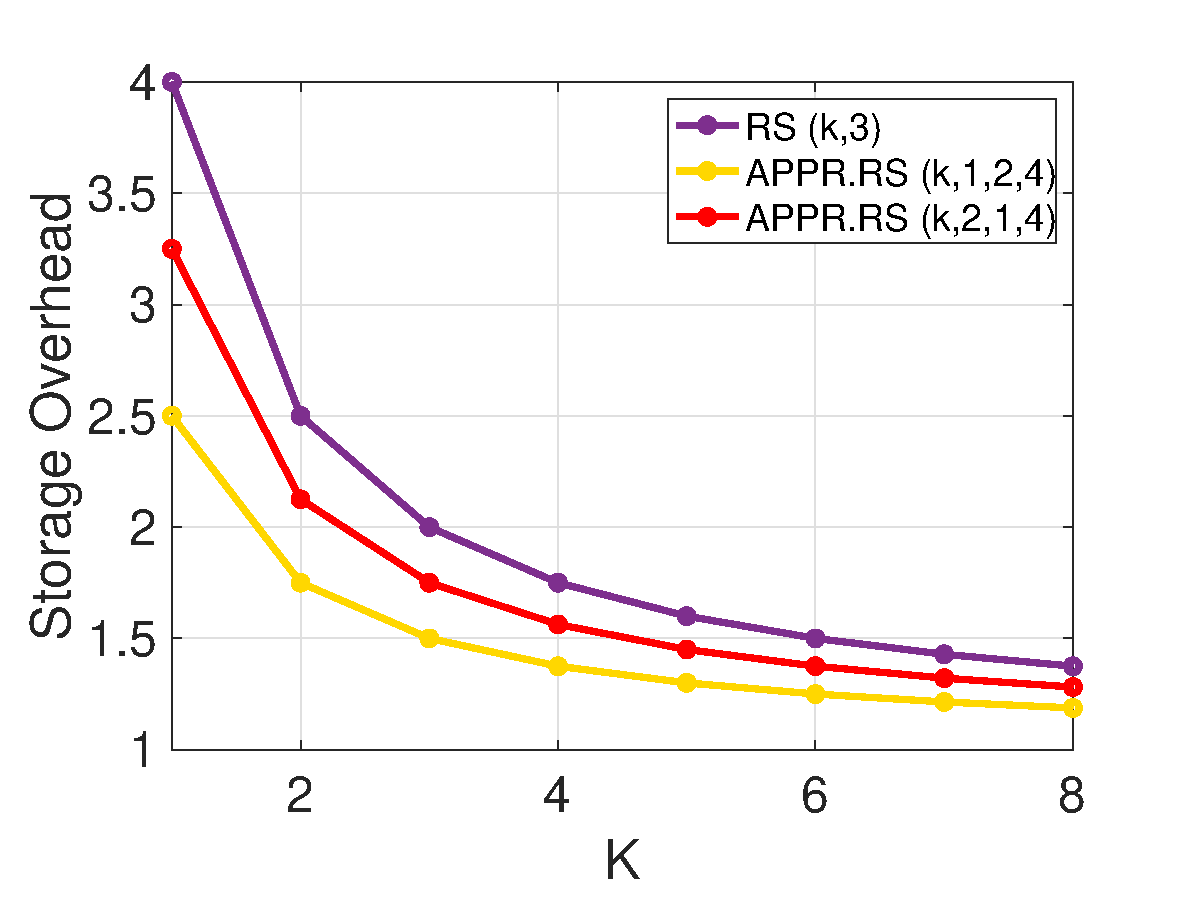
\includegraphics[width = 0.44\linewidth]{photo/experiment/Storage-4.eps}
}
\subfigure[h=6]{
    \label{fig-storage6}
    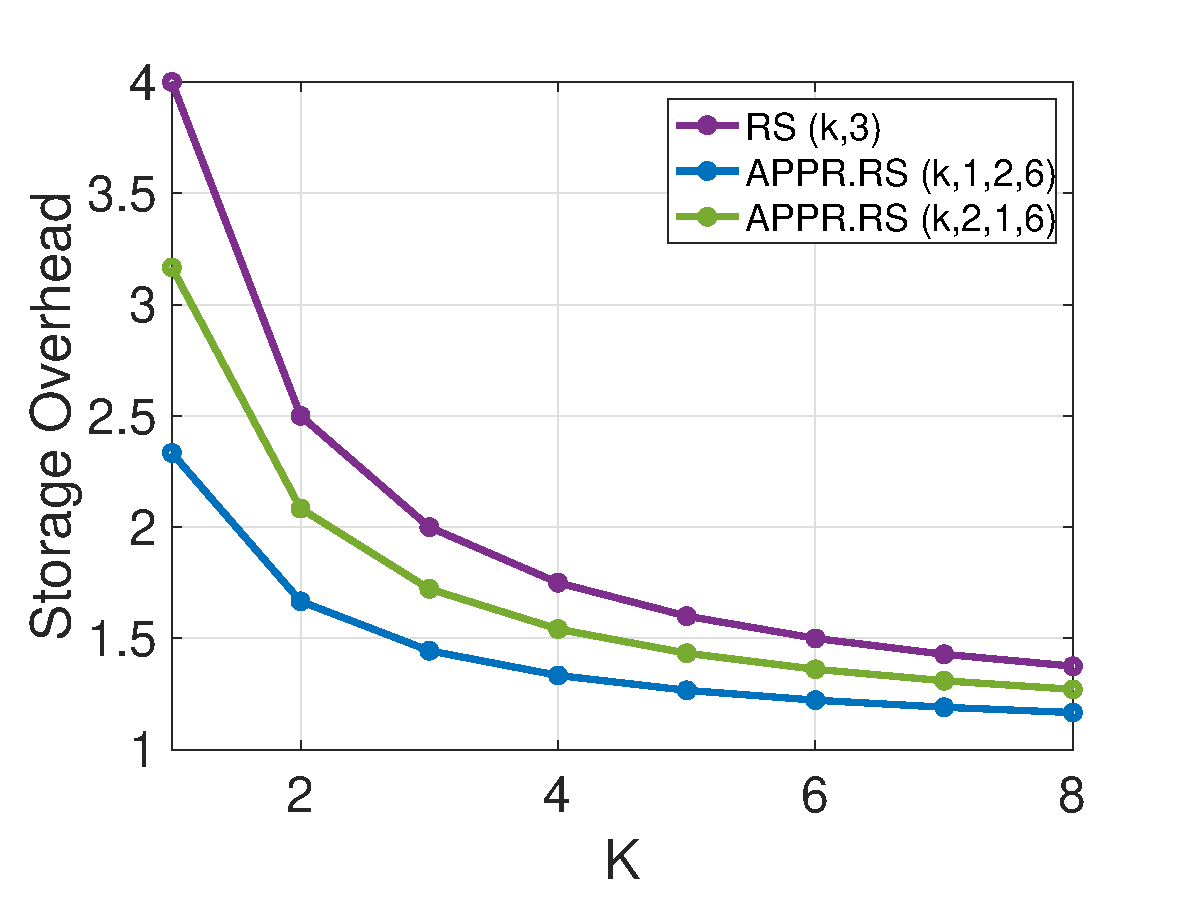
\includegraphics[width = 0.44\linewidth]{photo/experiment/Storage-6.eps}
}
\caption{Storage Overhead}\label{fig-Storage}
\end{figure}

\begin{figure}[ht]
\subfigure[h=4]{
    \label{fig-Sig-Write4}
    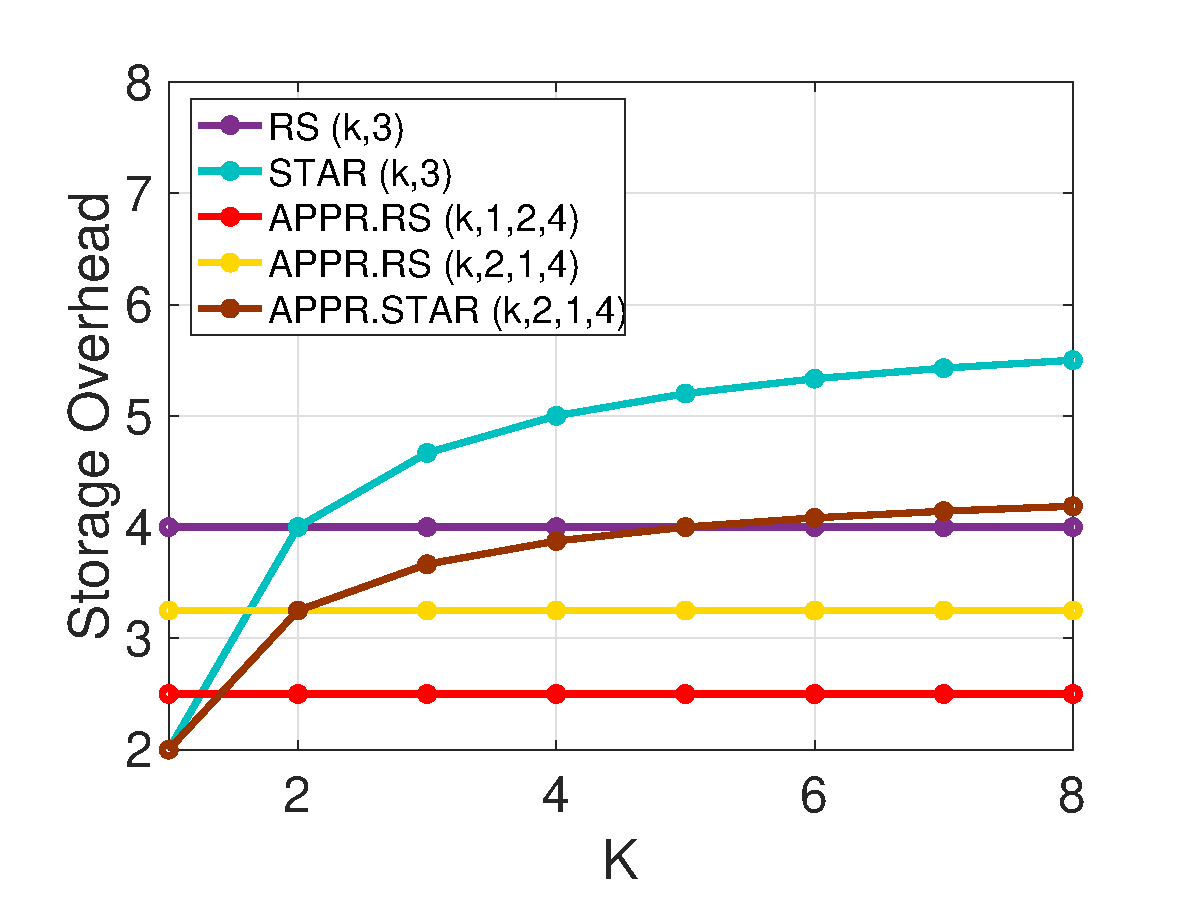
\includegraphics[width = 0.44\linewidth]{photo/experiment/Single-4.eps}
}
\subfigure[h=6]{
    \label{fig-Sig-Write6}
    \includegraphics[width = 0.44\linewidth]{photo/experiment/Single-6.eps}
}
\caption{Single Write Performance}\label{fig-Sig-Write}
\end{figure}

\subsection{Experimental Results Results and Analysis}
In this part, we compared the encoding and decoding time of Approximate Code with TIP code, STAR code, RS code and LRC codes, respectively. The code configuration is as follow,
\begin{itemize}
    \item \textbf{Approximate Code:} APPR.TIP/STAR ($k,1,2,4$), APPR. TIP/STAR ($k,2,1,4$), APPR. TIP/STAR ($k,1,2,6$), APPR.TIP/STAR ($k,2,1,6$). Since TIP and STAR code have different limits on the number of data nodes, we use these two codes to generate parities in Approximate Code, so that we can cover all the code configurations from $k$ = 5 to $k$ = 17. When we compare Approximate Code with STAR, we only choose APPR.STAR ($k,1,2,4$), APPR.STAR ($k,2,1,4$), APPR.STAR ($k,1,2,6$), APPR.STAR ($k,2,1,6$) and so do the TIP Code.
    \item \textbf{RS Code:} RS($k,3$). $k = 5,7,9,11,13$.
    \item \textbf{LRC Codes:} LRC ($k,4,3$), LRC ($k,6,3$). $k = 5,7,9,11,13$.
    \item \textbf{TIP Code:} TIP($k,3$). $k = 5,9,11,15,17$.
    \item \textbf{STAR Code:} STAR($k,3$). $k = 5,7,11,13,17$.
\end{itemize}
\subsubsection{Encoding Time}
The results are shown in Figure \ref{fig-encoding}.
\begin{itemize}
    \item STAR Code: Approximate Code encodes faster than STAR code and the rate of optimization is up to $56.3\%$ (between APPR.STAR ($k,1,2,6$) and STAR ($k,3$) when $k = 5$).

    \item TIP Code: the effet of TIP code is similar to STAR code. The rate of optimization is up to 58.1\% (between APPR.TIP($k,1,2,6$) and TIP($k,3$) when k = 9).

    \item RS Code: We could find out that the AP code encodes largely faster than RS code. The rate of optimization is up to 91.1\% (between APPR.TIP/STAR ($k,1,2,6$) and RS($k,3$) when $k = 5$).

    \item LRC Codes: We could see that Approximate Code largely reduces the encoding time, comparing to LRC codes. The rate of optimization is up to 88.9\% (between APPR.TIP/STAR ($k,1,2,6$) and LRC($k, 6, 2$) when $k = 5$).
\end{itemize}

We combined the encoding time of five codes in Figure \ref{fig-BAR} with $k$=5. The results show that Approximate Code has the best encoding performance among five codes. There are two reasons for this condition: (1) Approximate Code only generates $r+g/h$ parity nodes for each stripe, while tipical 3DFTs codes generate 3 nodes. (2) Approximate Code use XOR-based codes (TIP and STAR code) which have lower computational overhead than RS-based codes.\par

\begin{figure}[ht]
\subfigure{
    \label{fig-encodingSTAR}
    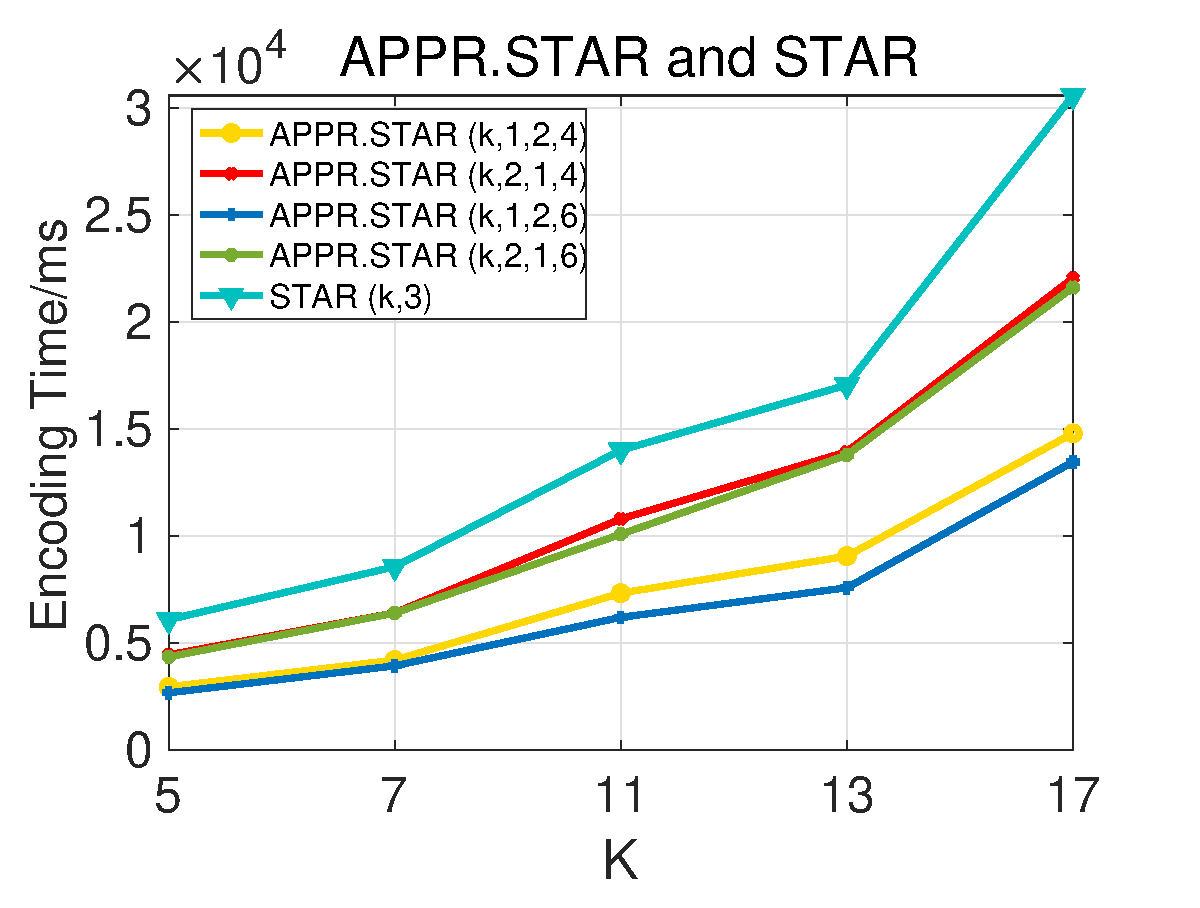
\includegraphics[width = 0.46\linewidth]{photo/experiment/Encoding-Star.eps}
}
\subfigure{
    \label{fig-encodingTIP}
    \includegraphics[width = 0.46\linewidth]{photo/experiment/Encoding-TIP.eps}
}
\subfigure{
    \label{fig-encodingRS}
    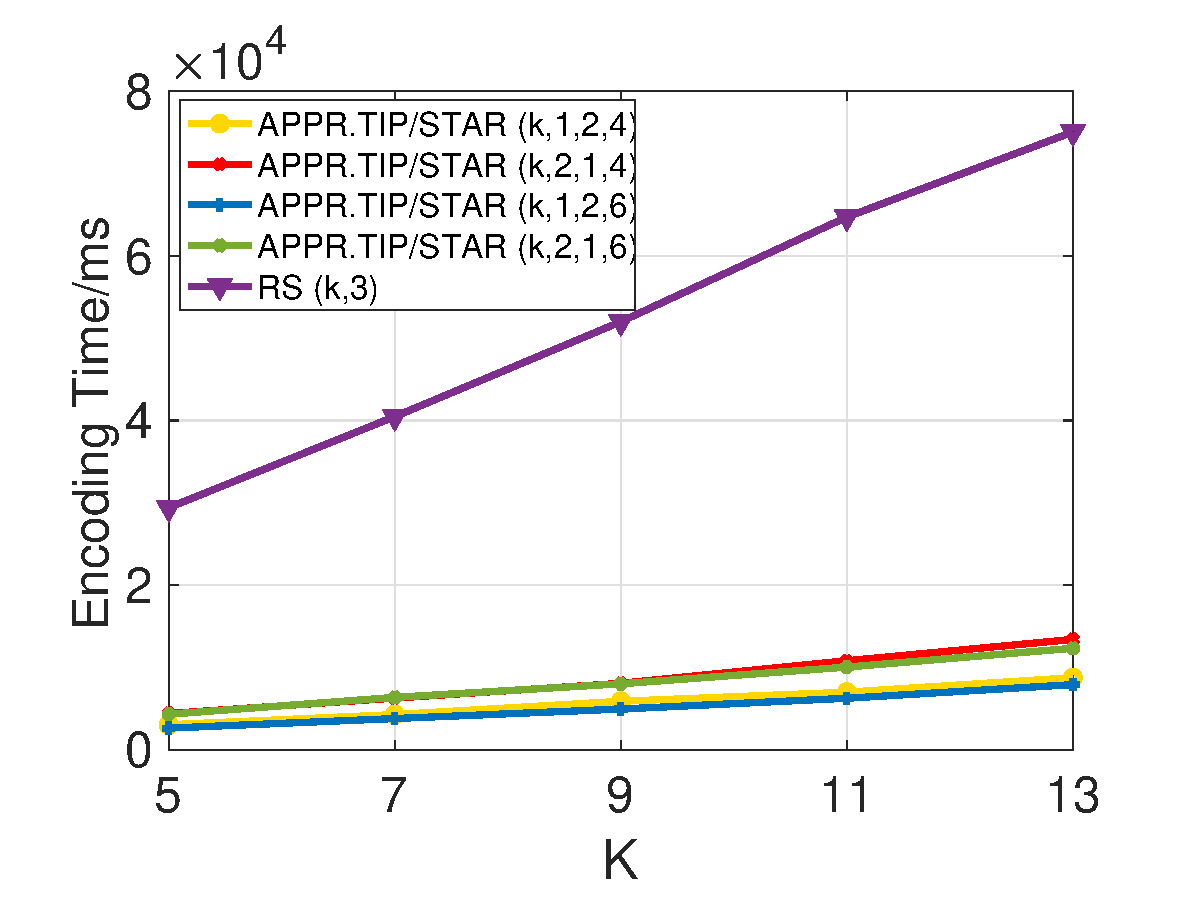
\includegraphics[width = 0.46\linewidth]{photo/experiment/Encoding-RS.eps}
}
\subfigure{
    \label{fig-encodingLRC}
    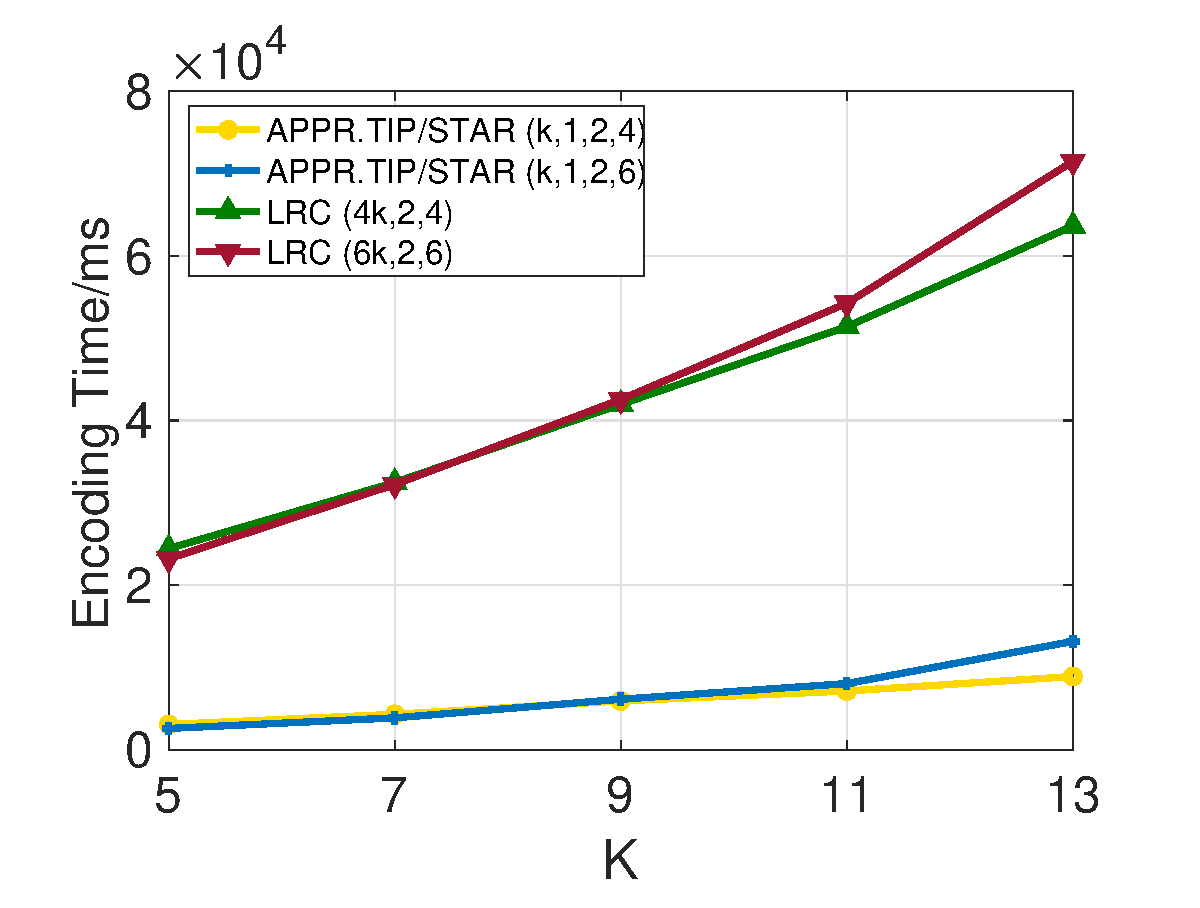
\includegraphics[width = 0.46\linewidth]{photo/experiment/Encoding-LRC.eps}
}
\vspace{-0.3cm}
\caption{Encoding Time Comparison between AP method and other method}\label{fig-encoding}
\end{figure}


\subsubsection{Decoding Time under Single Node Failure Condition Analysis}
The results are shown in Figure \ref{fig-decoding-1}.
\begin{itemize}
    \item STAR Code: The decoding time of Approximate Code is almost the same as STAR code when sinlge node fails and the rate of optimization is up to 5.4\% (between APPR.STAR ($k,1,2,4$) and STAR ($k,3$) when $k = 5$).
    \item TIP Code: The decoding time of Approximate Code is almost the same as TIP code when sinlge node fails and the rate of optimization is up to 8.8\% (between APPR.TIP($k,1,2,4$) and TIP($k,3$) when k = 17).
    \item RS Code: We could find out that the Approximate Code decodes largely faster than RS code. The rate of optimization is up to 80.2\% (between APPR.TIP/STAR ($k,1,2,4$) and RS($k,3$) when $k = 5$).
    \item LRC Codes: We could see that Approximate Code and LRC codes have no big gap when encoding one lost node. The rate of optimization is up to $5.8\%$ (between APPR.TIP/STAR ($k,1,2,6$) and LRC ($k, 6, 2$) when $k = 13$).
\end{itemize}

We combined the decoding time of five codes under one failure node condition in Figure \ref{fig-BAR} with $k=5$. The results show that RS code has the worst one node decoding performance among five codes and the performance of other four codes are almost the same. The main reason is that XOR-based codes have lower computational overhead than RS-based codes.\par

\begin{figure}[ht]
    \subfigure{
        \label{fig-decoding-1-STAR}
        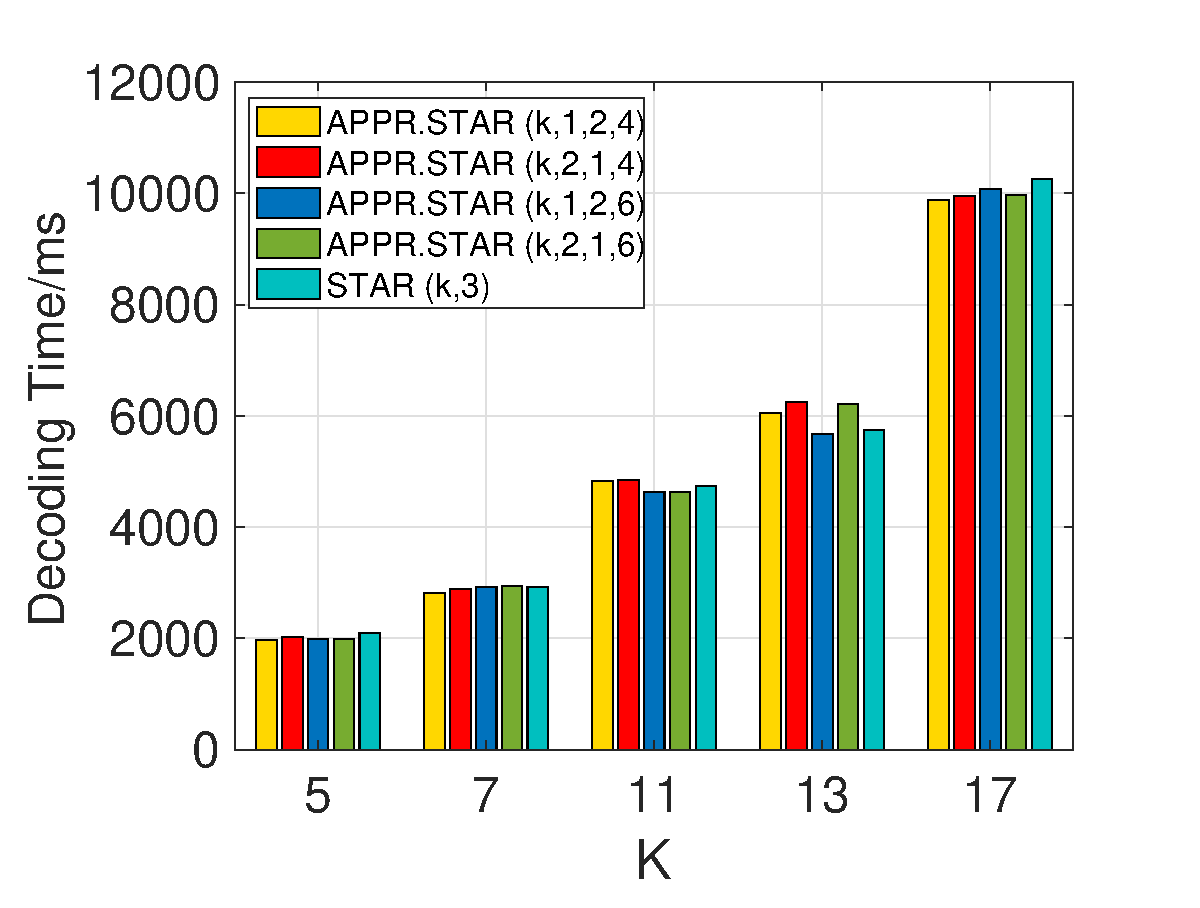
\includegraphics[width = 0.46\linewidth]{photo/experiment/Decoding-1-Star.eps}
    }
    \subfigure{
        \label{fig-decoding-1-TIP}
        \includegraphics[width = 0.46\linewidth]{photo/experiment/Decoding-1-TIP.eps}
    }
    \subfigure{
        \label{fig-decoding-1-RS}
        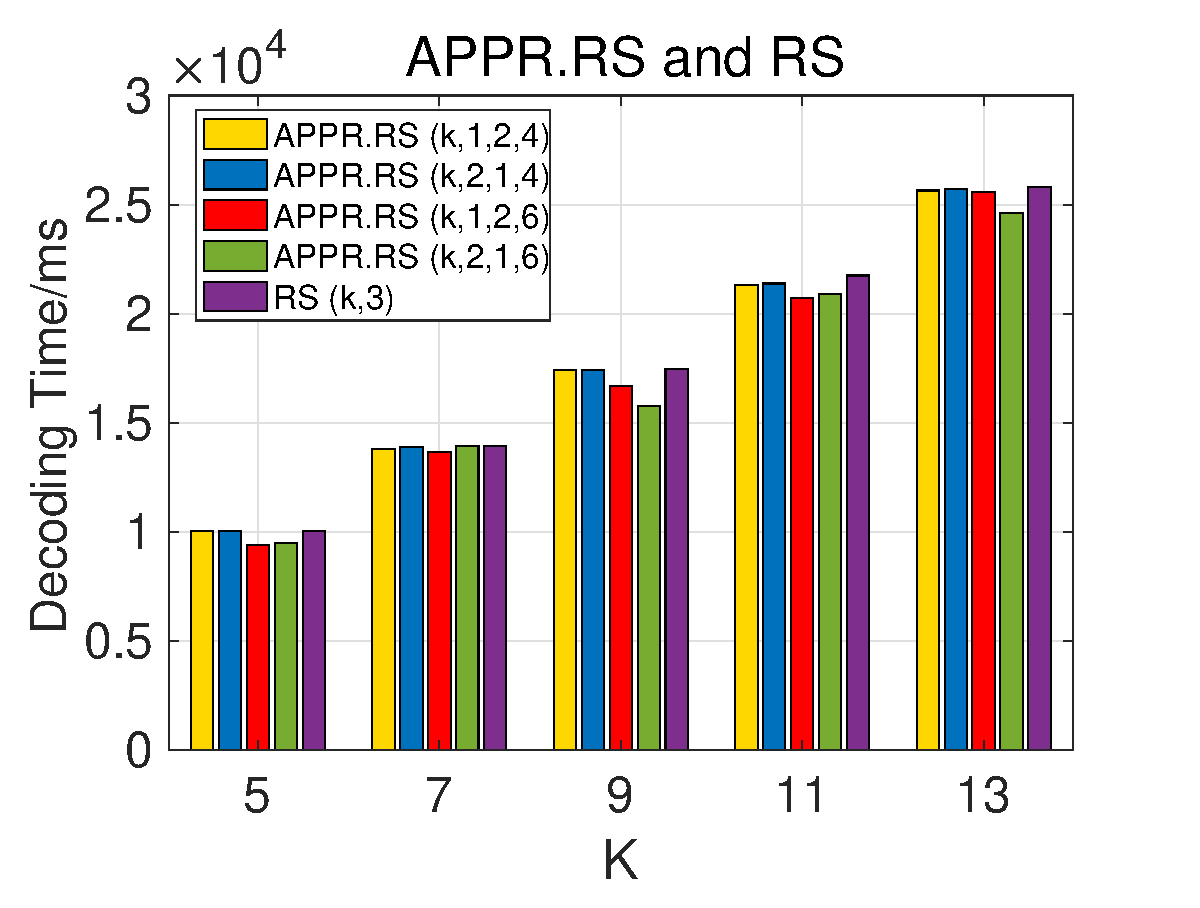
\includegraphics[width = 0.46\linewidth]{photo/experiment/Decoding-1-RS.eps}
    }
    \subfigure{
        \label{fig-decoding-1-LRC}
        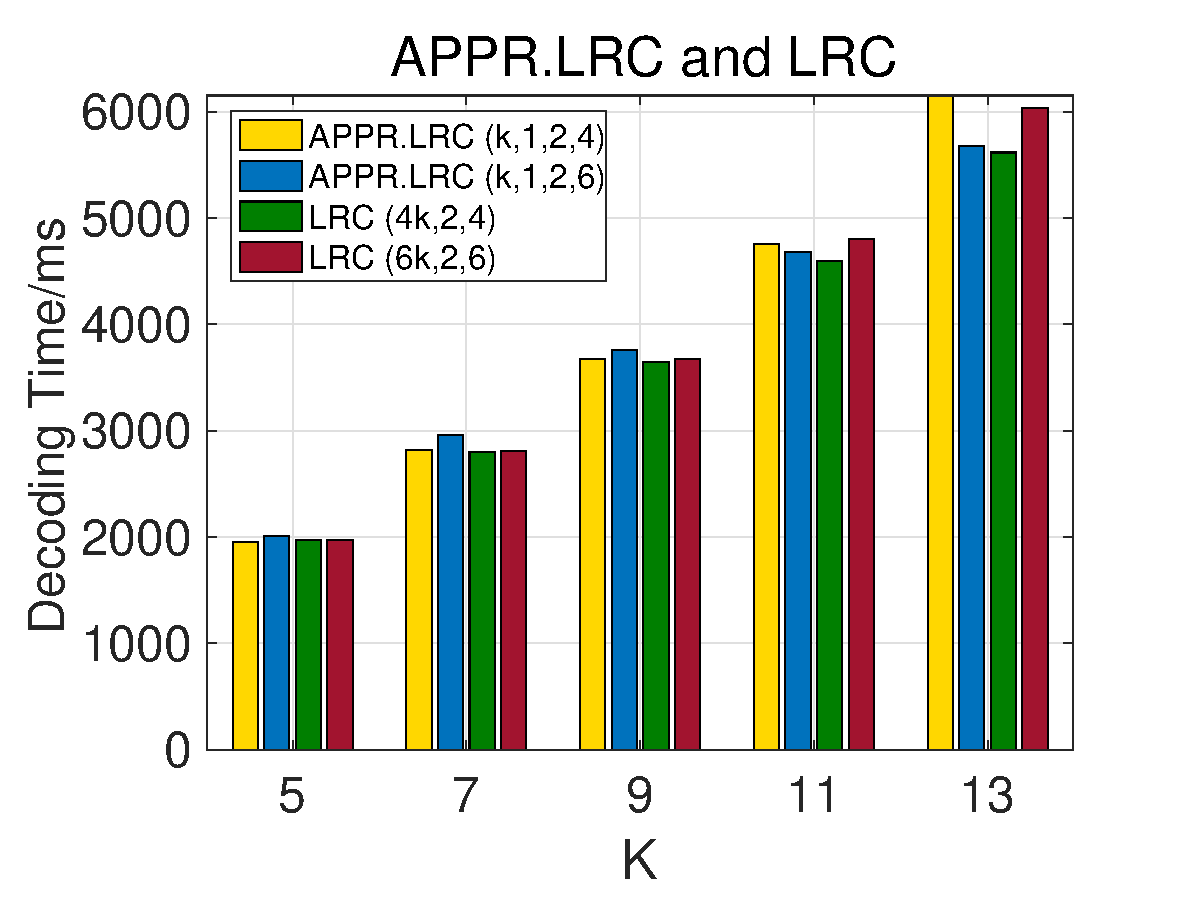
\includegraphics[width = 0.46\linewidth]{photo/experiment/Decoding-1-LRC.eps}
    }
    \vspace{-0.3cm}
    \caption{Decoding Time Comparison in Single Node Failure between Approximate Code and other method}\label{fig-decoding-1}
    \end{figure}

\subsubsection{Decoding Time under Double Node Failure Condition Analysis}
The results are shown in Figure \ref{fig-decoding-2}.
\begin{itemize}
    \item STAR Code: The rate of optimization is up to $83.9\%$ (between APPR.STAR ($k,1,2,6$) and STAR ($k,3$) when $k = 5$).
    \item TIP Code: This condition is similar to STAR code. The rate of optimization is up to $84.8\% $(between APPR.TIP($k,1,2,6$) and TIP($k,3$) when $k = 9$).
    \item RS Code: We could find out that the Approximate Code decodes largely faster than RS code under two failure nodes condition. The rate of optimization is up to $96.9\%$ (between APPR.TIP/STAR ($k,1,2,6$) and RS($k,3$) when $k = 5$).
    \item LRC Codes:
    We could see that Approximate Code largely reduces the decoding time when two nodes fail, compared with LRC codes. The rate of optimization is up to $97.2\%$ (between APPR.TIP/STAR ($k,1,2,6$) and LRC ($k, 6, 2$) when $k = 5$).
\end{itemize}

The combined decoding time of five codes under two failure node condition are shown in Figure \ref{fig-BAR} ($k=5$). The results show that RS code and LRC codes has the worst two failure nodes decoding performance while APPR.TIP/STAR ($k,1,2,6$) and APPR.TIP/STAR ($k,1,2,4$) perform best among all kinds of codes. The main reasons are that: On two failure nodes condition, RS code and LRC codes decode data based on RS method which have heavy computational cost while APPR.TIP/STAR ($k,1,2,6$) and APPR.TIP/STAR ($k,1,2,4$) do the approximate recovery which means they only recover important data at this time.

\begin{figure}[ht]
    \subfigure{
        \label{fig-decoding-2-STAR}
        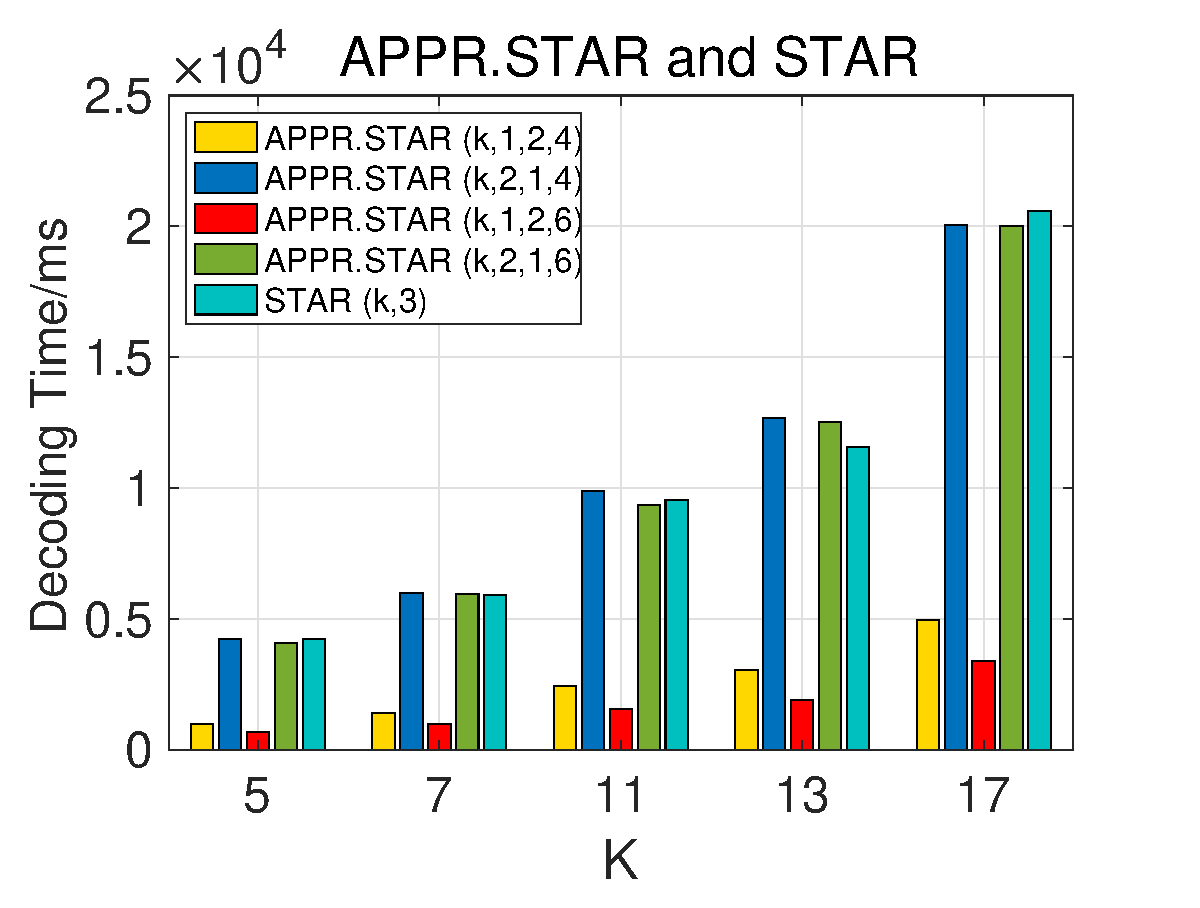
\includegraphics[width = 0.46\linewidth]{photo/experiment/Decoding-2-Star.eps}
    }
    \subfigure{
        \label{fig-decoding-2-TIP}
        \includegraphics[width = 0.46\linewidth]{photo/experiment/Decoding-2-TIP.eps}
    }
    \subfigure{
        \label{fig-decoding-2-RS}
        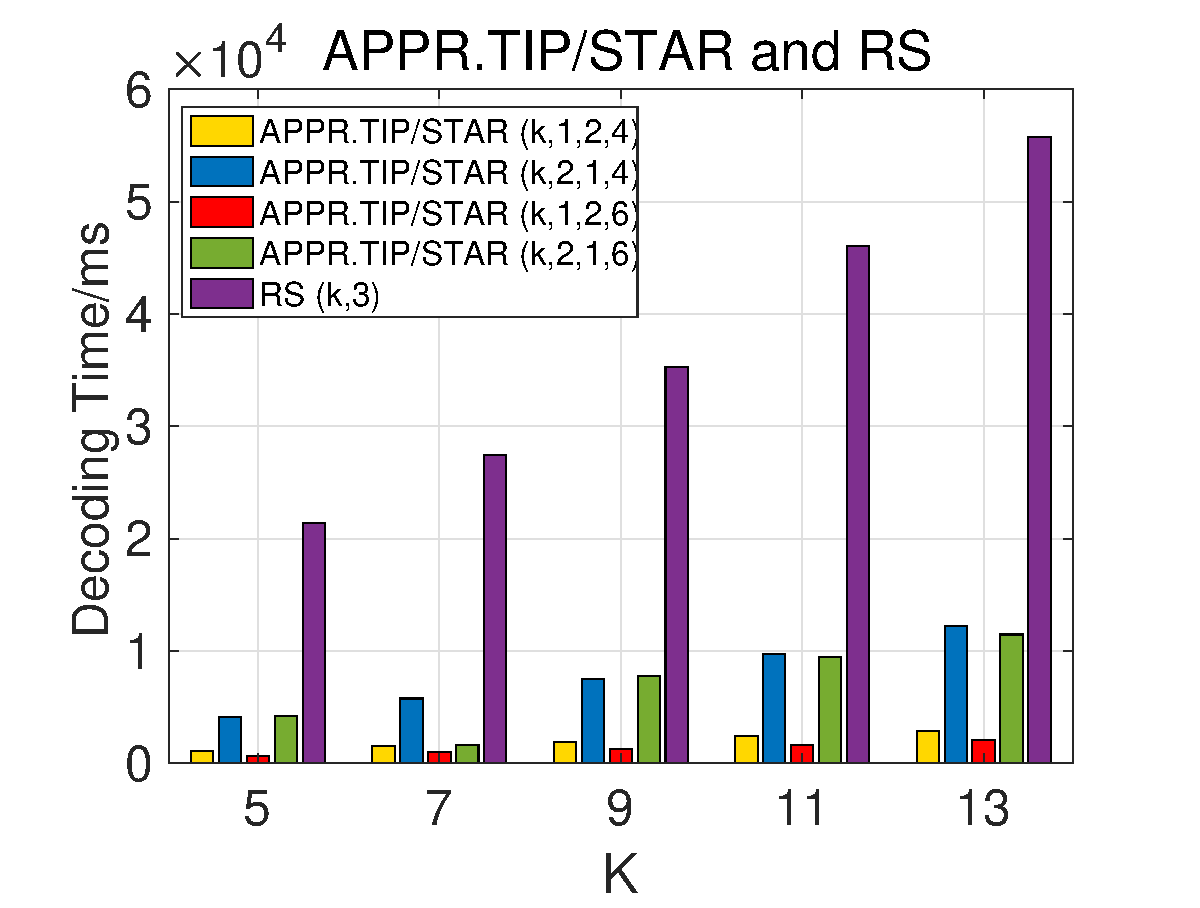
\includegraphics[width = 0.46\linewidth]{photo/experiment/Decoding-2-RS.eps}
    }
    \subfigure{
        \label{fig-decoding-2-LRC}
        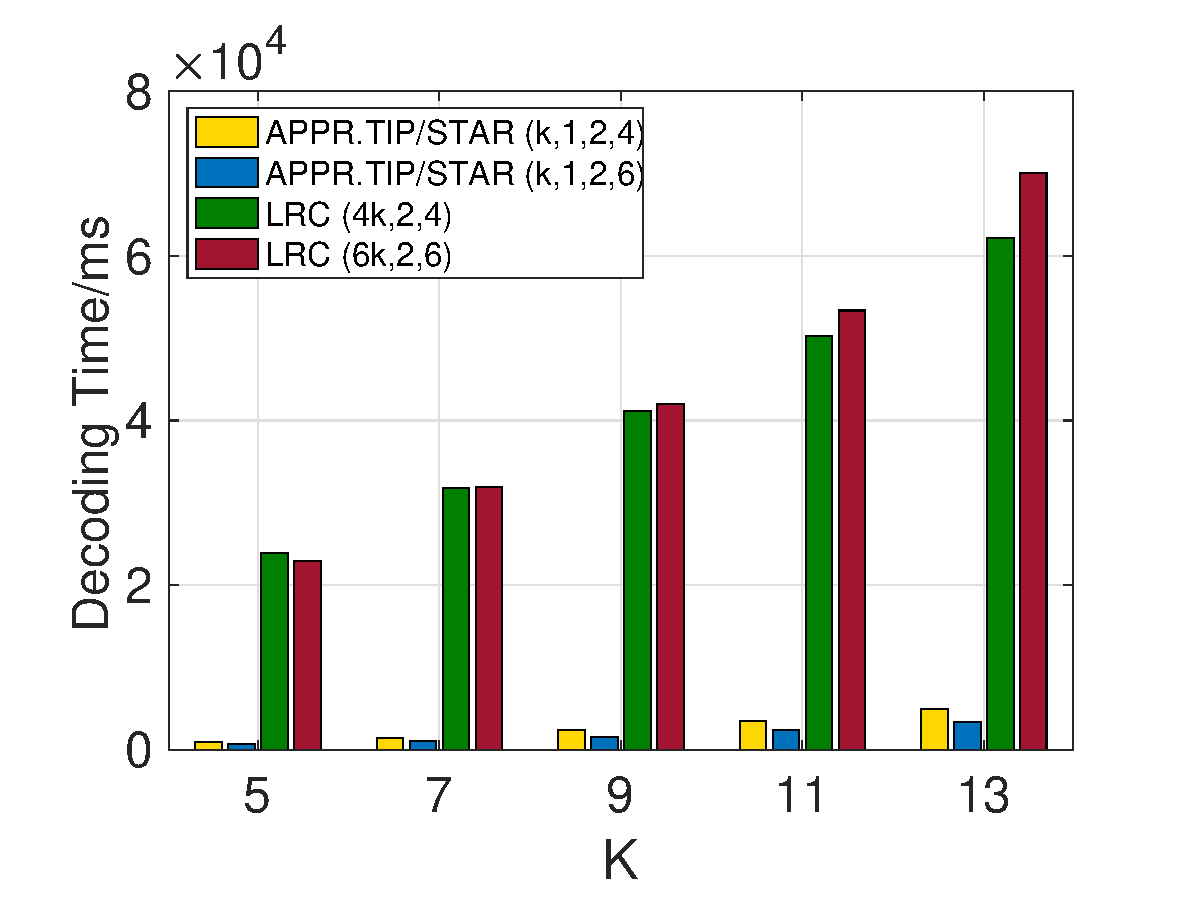
\includegraphics[width = 0.46\linewidth]{photo/experiment/Decoding-2-LRC.eps}
    }
    \vspace{-0.3cm}
    \caption{Decoding Time Comparison in Double Node Failure between Approximate Code and other method}\label{fig-decoding-2}
    \end{figure}

\subsubsection{Decoding Time under Triple Node Failure Condition Analysis}
The results are shown in Figure \ref{fig-decoding-3}.
\begin{itemize}
    \item STAR Code: the rate of optimization is up to $83.5\%$ (between APPR.STAR ($k,1,2,6$) and STAR ($k,3$) when $k = 5$).
    \item TIP Code: This condition is similar to STAR code. The rate of optimization is up to 82.2\% (between APPR.TIP($k,1,2,6$) and TIP($k,3$) when $k = 5$).
    \item RS Code: We could find out that the Approximate Code decodes largely faster than RS code under three failure nodes condition. The rate of optimization is up to $96.7\%$ (between APPR.TIP/STAR ($k,1,2,6$) and RS($k,3$) when $k = 5$).
    \item LRC Codes:
    We could see that Approximate Code largely reduces the decoding time when three nodes fail, compared with LRC codes. The rate of optimization is up to $98.3\%$  (between APPR.TIP/STAR ($k,1,2,6$) and LRC ($k, 6, 2$) when $k = 5$).
\end{itemize}

The combined decoding time of five codes under three failure node condition are shown in Figure \ref{fig-BAR} ($k$=5). The results show that LRC has the worst three failure nodes decoding performance. The main reasons are that: On three failure nodes condition, LRC codes decode data through the global parities which has a longer parity chain. For example $LRC (44,4,2)$ use 44 nodes to recover the three lost nodes. the computational cost of GF operations is also larger than XOR operations. On the other hand, All kinds of Approximate Code perform best among all kinds of codes because they only recover important data at this time.

\begin{figure}[ht]
    \subfigure{
        \label{fig-decoding-3-STAR}
        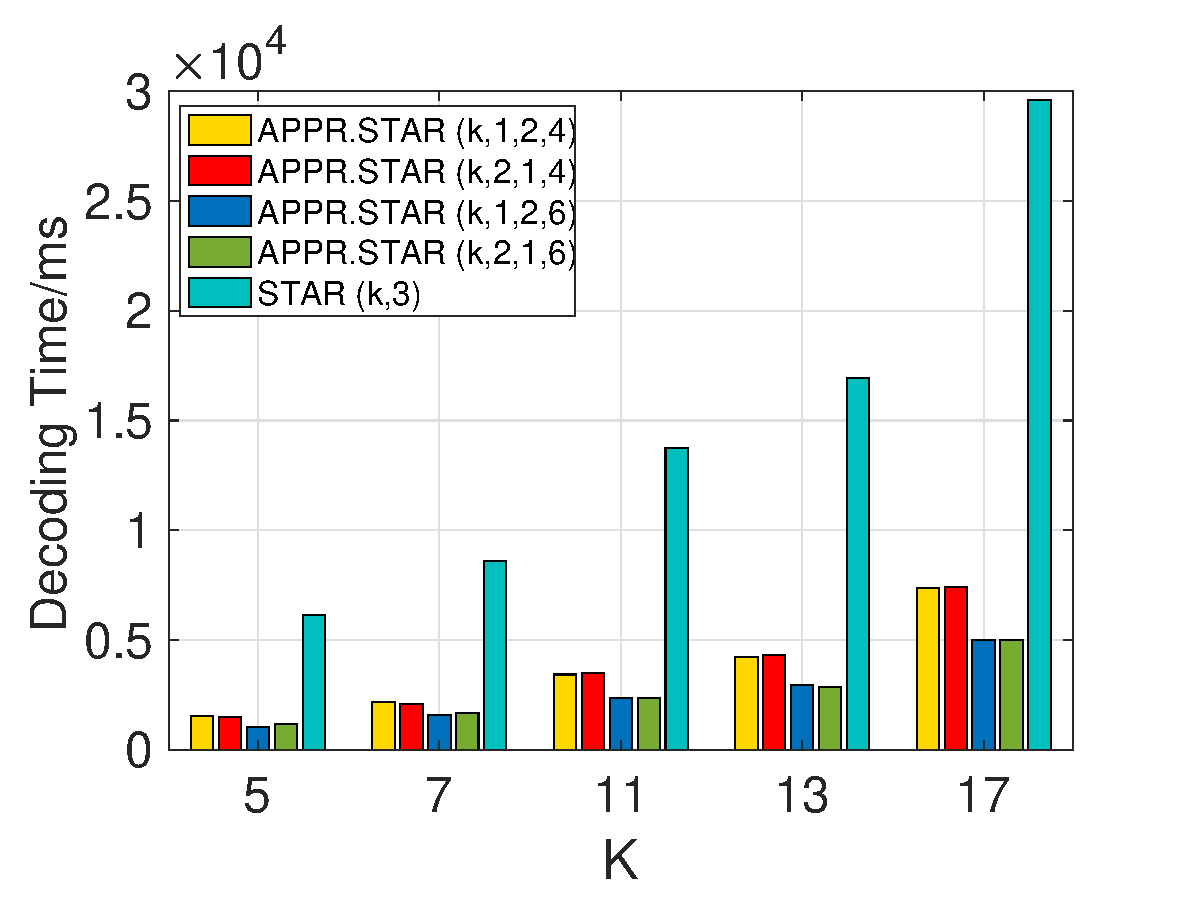
\includegraphics[width = 0.46\linewidth]{photo/experiment/Decoding-3-Star.eps}
    }
    \subfigure{
        \label{fig-decoding-3-TIP}
        \includegraphics[width = 0.46\linewidth]{photo/experiment/Decoding-3-TIP.eps}
    }
    \subfigure{
        \label{fig-decoding-3-RS}
        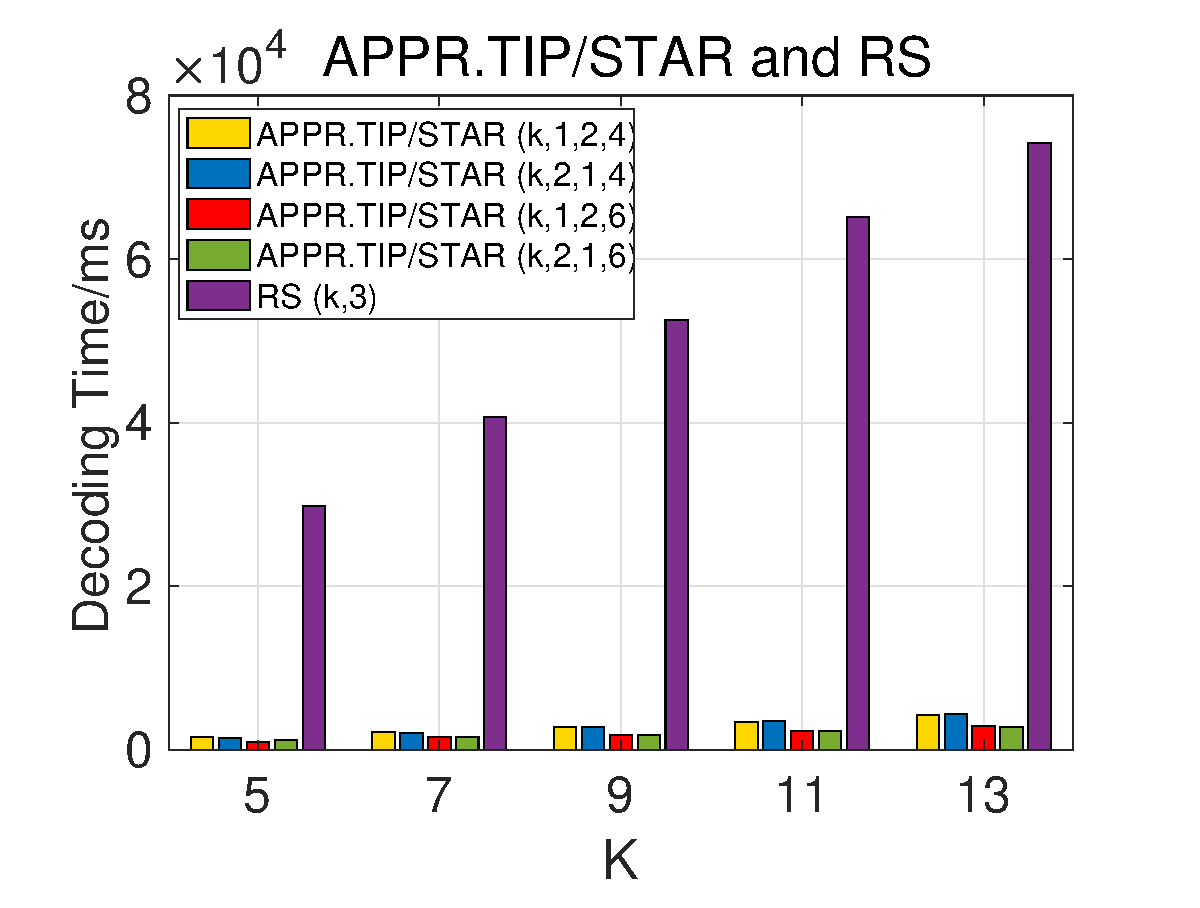
\includegraphics[width = 0.46\linewidth]{photo/experiment/Decoding-3-RS.eps}
    }
    \subfigure{
        \label{fig-decoding-3-LRC}
        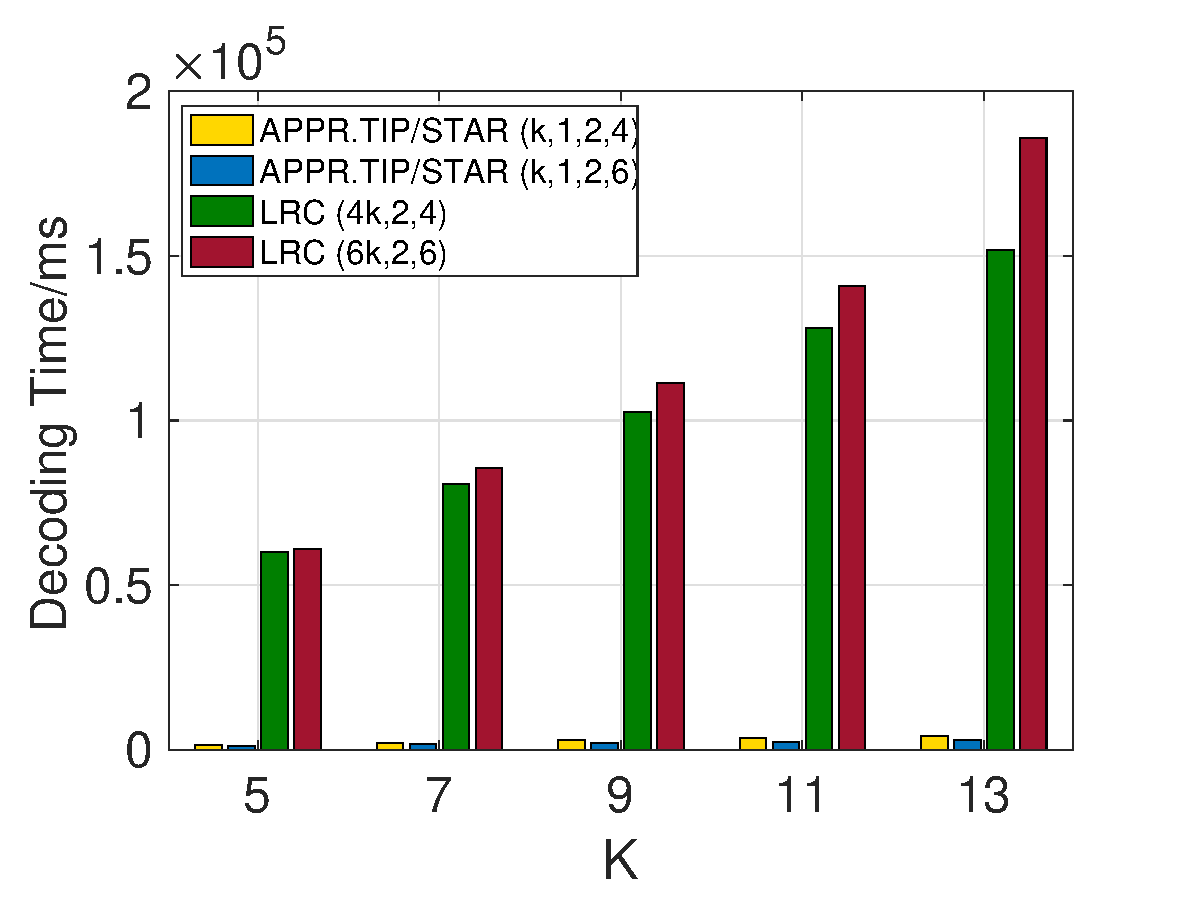
\includegraphics[width = 0.46\linewidth]{photo/experiment/Decoding-3-LRC.eps}
    }
    \vspace{-0.3cm}
    \caption{Decoding Time Comparison in Triple Node Failure between Approximate Code and other method}\label{fig-decoding-3}
    \end{figure}

\begin{figure*}[!ht]
    \subfigure{
        \label{fig-encoding-combine}
        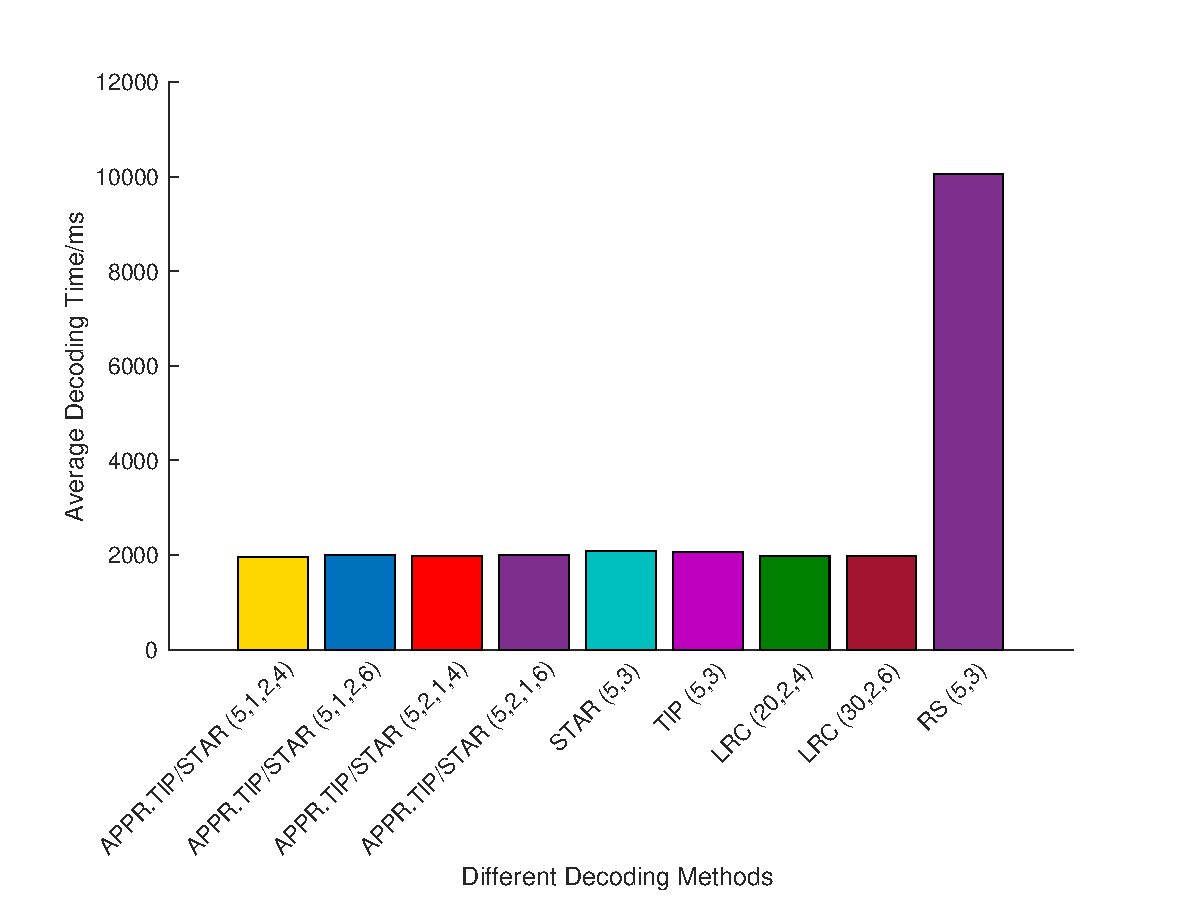
\includegraphics[width = 0.23\linewidth]{photo/experiment/Bar-Encoding.eps}
    }
    \subfigure{
        \label{fig-decoding-1-combine}
        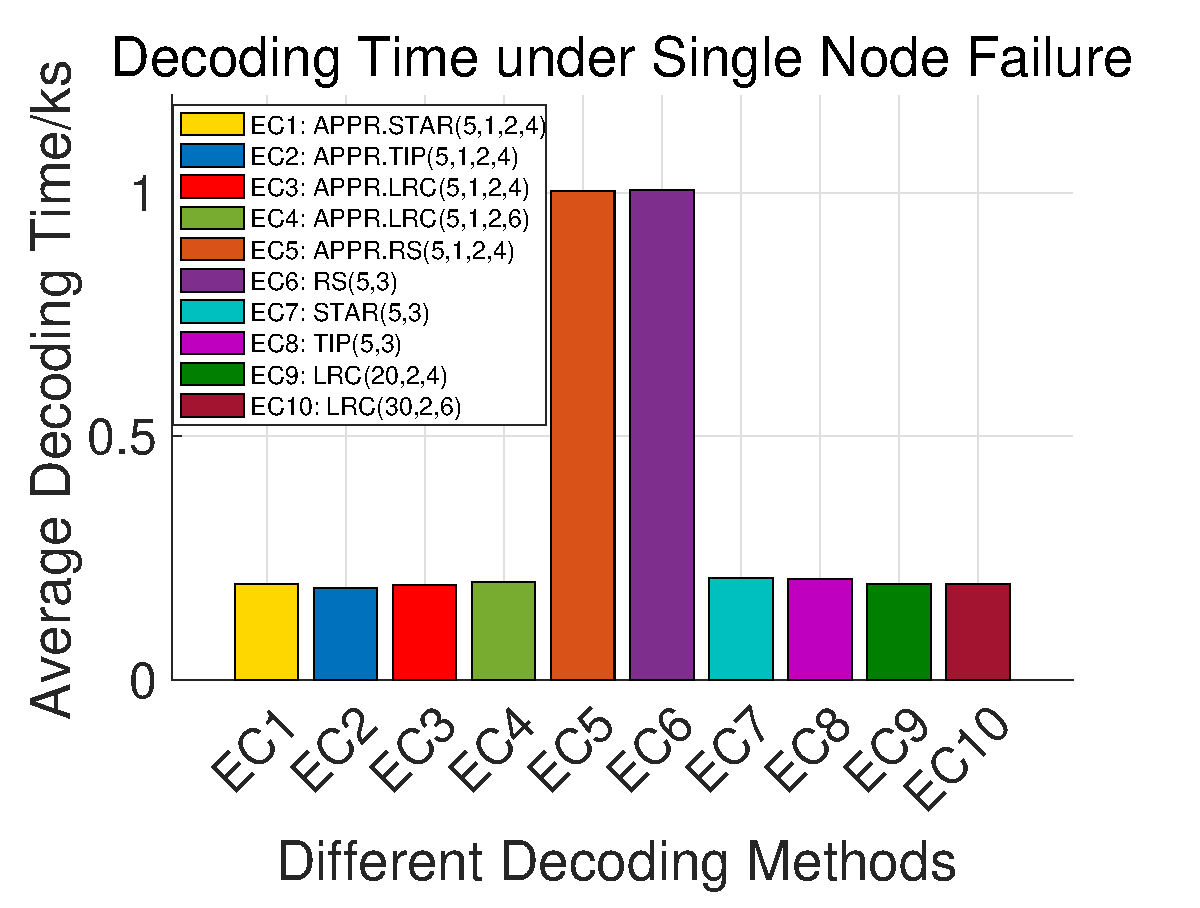
\includegraphics[width = 0.23\linewidth]{photo/experiment/Bar-Decoding-1.eps}
    }
    \subfigure{
        \label{fig-decoding-2-combine}
        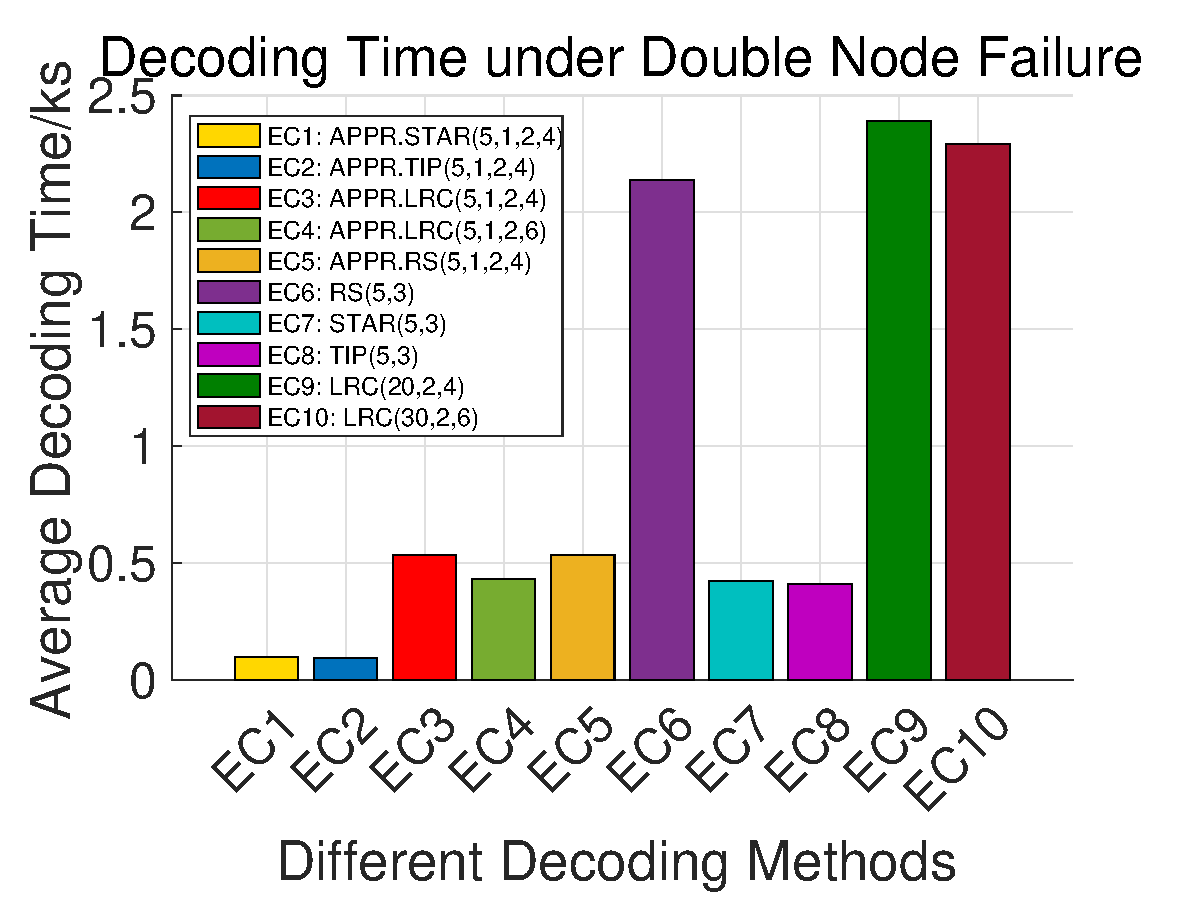
\includegraphics[width = 0.23\linewidth]{photo/experiment/Bar-Decoding-2.eps}
    }
    \subfigure{
        \label{fig-decoding-3-combine}
        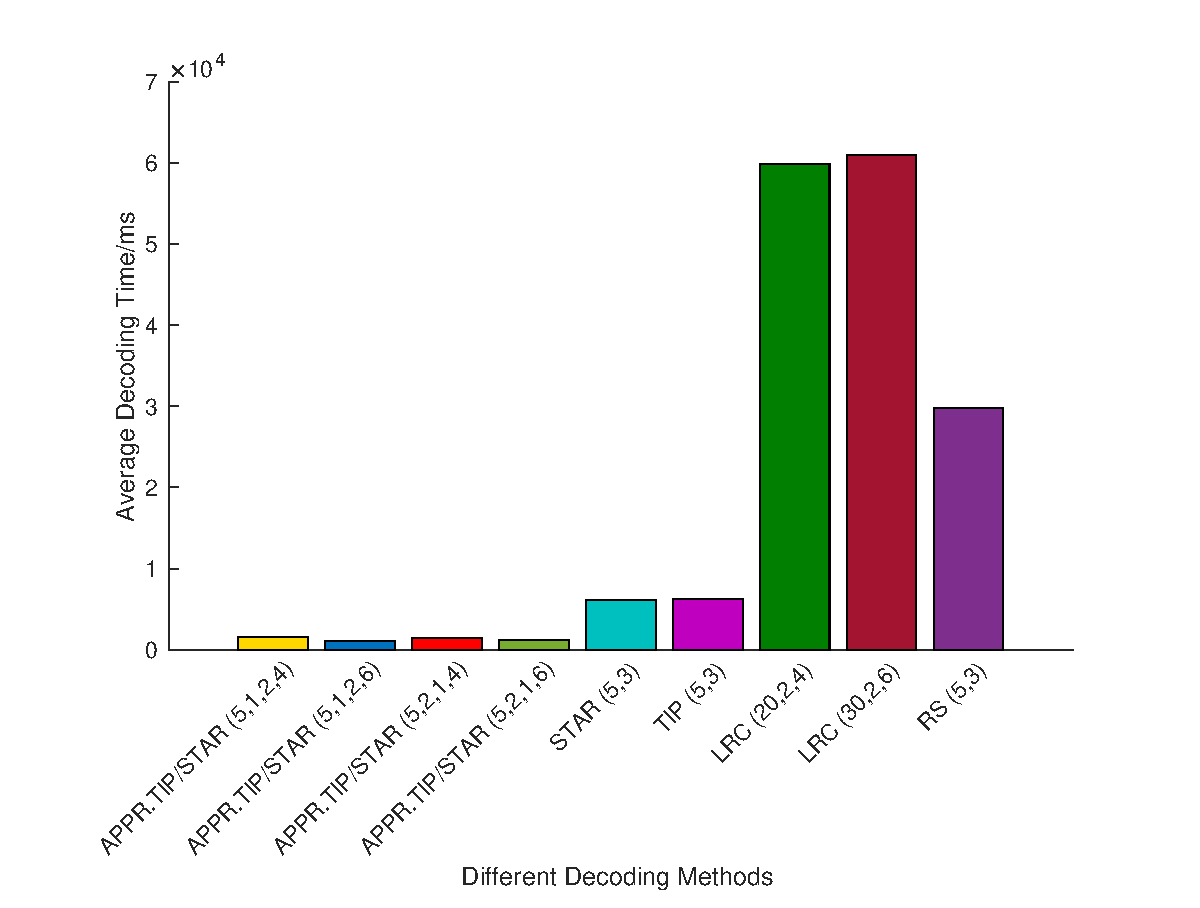
\includegraphics[width = 0.23\linewidth]{photo/experiment/Bar-Decoding-3.eps}
    }
    \caption{Comparison of several matrics between different methods when the number of data nodes is 5}\label{fig-BAR}
    \end{figure*}

\subsubsection{Recovery Time Analysis}

Figure \ref{fig-recovery} shows the recovery time of Approximate Code and other ECs under two and three failure nodes
condition. We can see that Approximate Code owns the best recovery performance in all ECs. The optimization ratio can be up to 97.7\% between APPR.TIP/STAR(5,1,2,6) and LRC(30,2,6). The main reason is that Approximate Code only recover important data under multiple failure nodes condition which can significantly reduce computation time, I/O overhead and transmission time.

\begin{figure}[ht]
    \subfigure{
        \label{fig-recovery-2}
        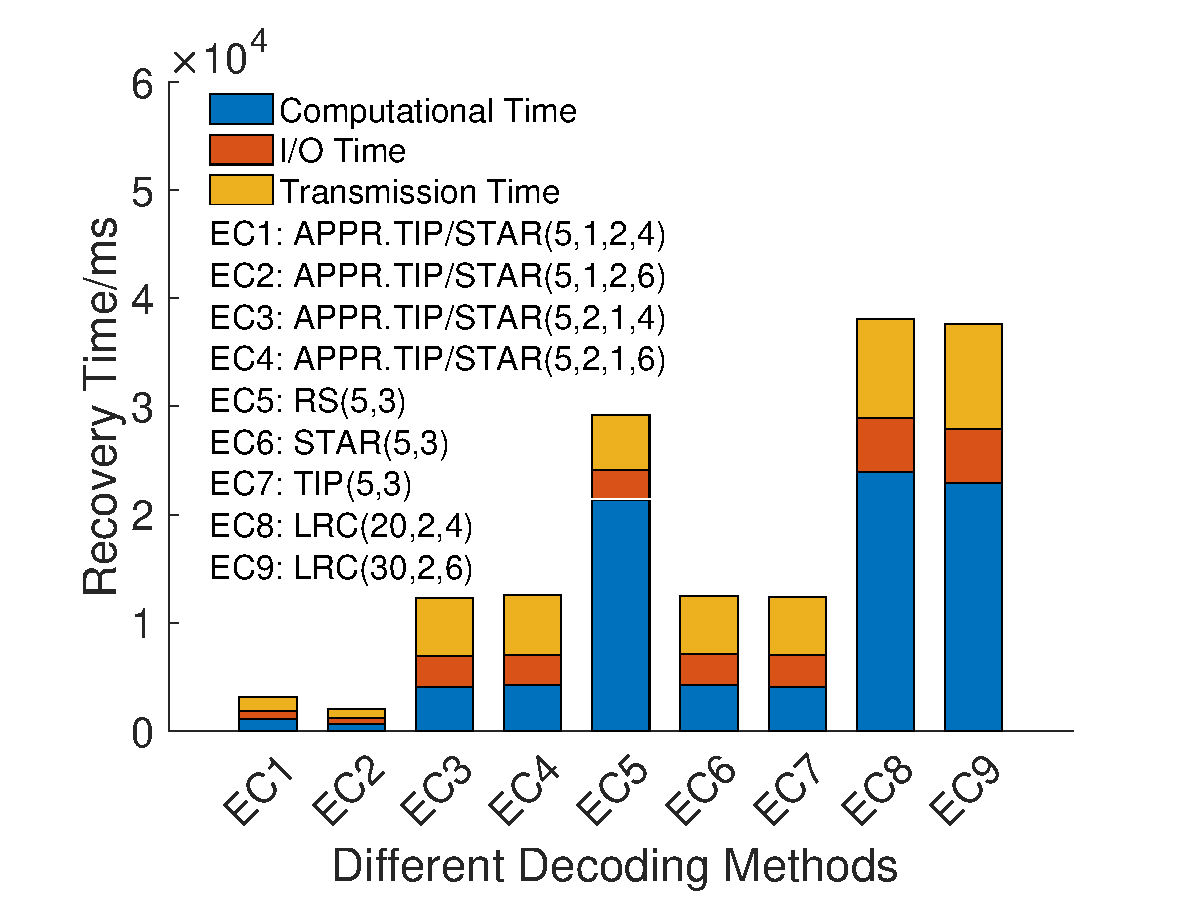
\includegraphics[width = 0.46\linewidth]{photo/experiment/Recovery-2.eps}
    }
    \subfigure{
        \label{fig-recovery-3}
        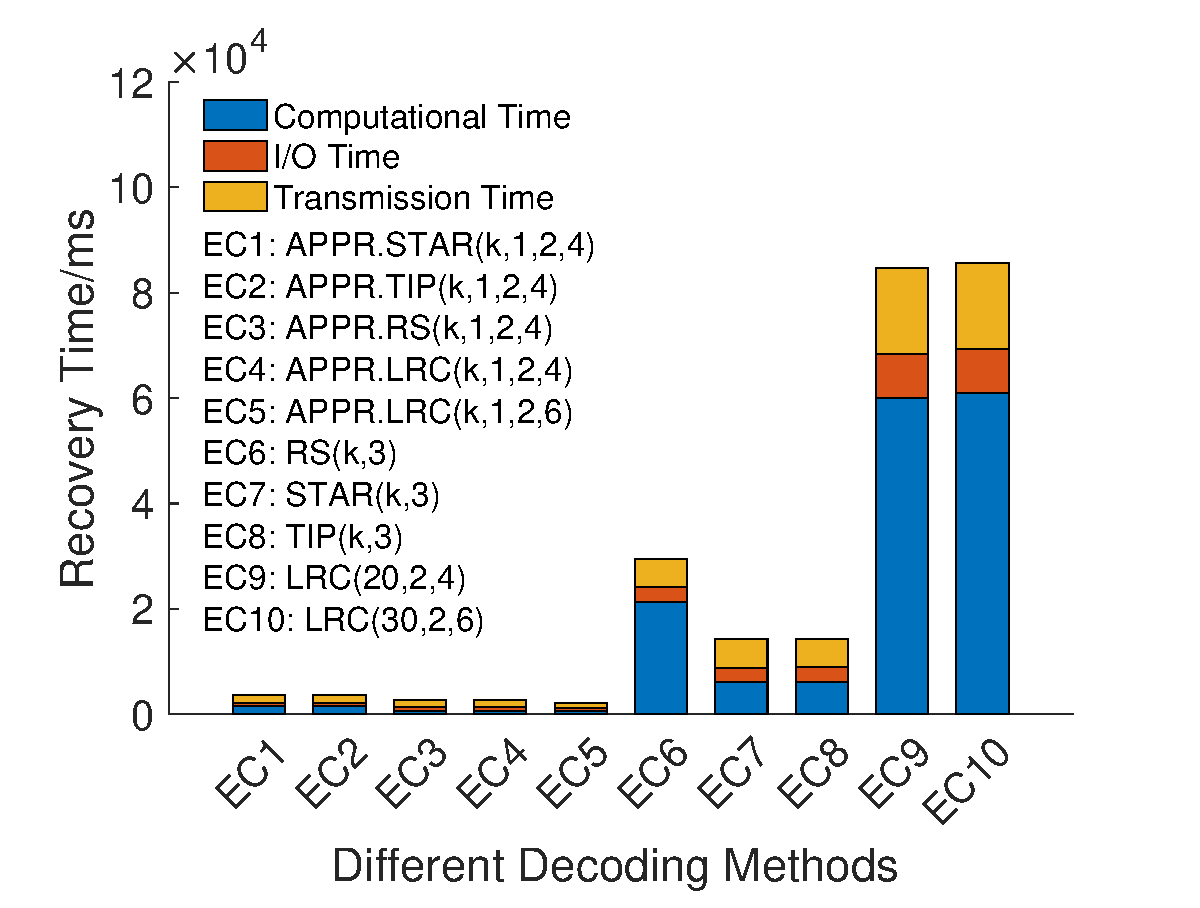
\includegraphics[width = 0.46\linewidth]{photo/experiment/Recovery-3.eps}
    }
    \vspace{-0.3cm}
    \caption{Recovery time comparison in double and triple node failures between Approximate Code and other ECs}\label{fig-recovery}
    \end{figure}

\subsection{Frame Recovery}
Here we present the frame recovery result by using frame interpolation \cite{meyer2015phase, niklaus2018context,van2017frame}. As shown in Figure\ref{fig-frameRecovery}, The top 3 figures are the original frames. When frame 2 lost, the interpolation techniques can output \ref{fig-recoverof2} by the input of \ref{fig-interop1} and \ref{fig-interop3}. The recovered frame has a lower resolution and may differ from the original image, but since the unconstrained frame contains most of the context information, the video is still available, which validates the fact that the video can tolerate a certain amount of data loss.

\begin{figure}[ht]
\centering
\subfigure[Frame 1]{

\includegraphics[width=0.3\linewidth]{photo/Frame/1.jpg}\label{fig-interop1}
}
\subfigure[Frame 2]{

\includegraphics[width=0.3\linewidth]{photo/Frame/2.jpg}\label{fig-interop2}
}
\subfigure[Frame 3]{

\includegraphics[width=0.3\linewidth]{photo/Frame/3.jpg}\label{fig-interop3}
}

\subfigure[Recovery of Frame 2]{

\includegraphics[width=0.5\linewidth]{photo/Frame/2_1.jpg}\label{fig-recoverof2}
}
\caption{Frame Recovery Result using Frame Interpolation}
\label{fig-frameRecovery}
\end{figure}

\subsection{Analysis}
The improvements of Approximate Code over STAR/TIP/RS/LRC codes are listed in Table \ref{tab-summary}. From the table, we discover that Approximate Code can obtain a better encoding/decoding performance in all experiments. There are several reasons to achieve these gains. First, Approximate Code only provides three parities for important data and this method leads to the improvements of storage efficiency and encoding/decoding performance. Secondly Approximate Code uses XOR-Based codes to generate parities which reduce the computation overhead. Finally, the parity chain of Approximate Code is shorter than other ECs and takes advantage of transmission time and I/O overhead in cloud storage systems.


\begin{table}[]\footnotesize
\caption{Summary on various of configurations of APPR.TIP/STAR Code}\label{tab-summary}
\begin{tabular}{|p{1.5cm}<{\centering}|p{1.2cm}<{\centering}|c|c|c|c|c|}
\hline
\multirow{2}{*}{\begin{tabular}[c]{@{}c@{}}Experiment\\ scenario\end{tabular}} & \multirow{2}{*}{\begin{tabular}[c]{@{}c@{}}Coding\\ Method\end{tabular}} & \multicolumn{5}{c|}{Number of Nodes $k$} \\ \cline{3-7} 
 &  & \multicolumn{1}{c|}{5} & \multicolumn{1}{c|}{7} & \multicolumn{1}{c|}{9} & \multicolumn{1}{c|}{11} & \multicolumn{1}{c|}{13} \\ \hline
\multirow{4}{*}{Encoding} & \multicolumn{6}{c|}{APPR.TIP/STAR(5,1,2,4)} \\ \cline{2-7} 
 & RS (k,3) & 89.7\% & 89.5\% & 88.7\% & 89.2\% & 88.3\% \\ \cline{2-7} 
 & Star (k,3) & 51.6\% & 51.0\% & 48.4\% & 46.9\% & 51.7\% \\ \cline{2-7} 
 & LRC (20,2,4) & 87.5\% & 86.8\% & 85.9\% & 86.1\% & 86.0\% \\ \hline
\multirow{4}{*}{Encoding} & \multicolumn{6}{c|}{APPR.TIP/STAR (5,1,2,6)} \\ \cline{2-7} 
 & RS (k,3) & 91.1\% & 90.7\% & 90.5\% & 90.3\% & 89.5\% \\ \cline{2-7} 
 & Star (k,3) & 56.3\% & 54.2\% & / & 55.8\% & 55.6\% \\ \cline{2-7} 
 & LRC (30,2,6) & 88.9\% & 88.0\% & 85.6\% & 85.2\% & 81.6\% \\ \hline
\multirow{8}{*}{\begin{tabular}[c]{@{}c@{}}Decoding under\\ Single Node \\ Failure\end{tabular}} & \multicolumn{6}{c|}{APPR.TIP/STAR(5,1,2,4)} \\ \cline{2-7} 
 & RS (k,3) & 79.6\% & 79.3\% & 78.7\% & 78.2\% & 78.0\% \\ \cline{2-7} 
 & Star (k,3) & 5.5\% & 3.7\% & -2.1\% & -5.3\% & 3.7\% \\ \cline{2-7} 
 & LRC (20,2,4) & 1.3\% & -0.8\% & -0.9\% & -3.5\% & -9.5\% \\ \cline{2-7} 
 & \multicolumn{6}{c|}{APPR.TIP/STAR (5,1,2,6)} \\ \cline{2-7} 
 & RS (k,3) & 80.1\% & 79.4\% & 78.7\% & 77.6\% & 76.0\% \\ \cline{2-7} 
 & Star (k,3) & 5.1\% & -0.5\% & / & 2.1\% & 1.4\% \\ \cline{2-7} 
 & LRC (30,2,6) & -1.9\% & -5.4\% & -1.9\% & 3.5\% & 5.8\% \\ \hline
\multirow{8}{*}{\begin{tabular}[c]{@{}c@{}}Decoding under\\ Double Node\\ Failure\end{tabular}} & \multicolumn{6}{c|}{APPR.TIP/STAR(5,1,2,4)} \\ \cline{2-7} 
 & RS (k,3) & 94.9\% & 94.5\% & 94.6\% & 94.8\% & 94.8\% \\ \cline{2-7} 
 & Star (k,3) & 76.5\% & 76.0\% & 74.5\% & 73.7\% & 76.0\% \\ \cline{2-7} 
 & LRC (20,2,4) & 96.0\% & 95.5\% & 94.1\% & 93.0\% & 92.0\% \\ \cline{2-7} 
 & \multicolumn{6}{c|}{APPR.TIP/STAR (5,1,2,6)} \\ \cline{2-7} 
 & RS (k,3) & 96.9\% & 96.5\% & 96.5\% & 96.5\% & 96.3\% \\ \cline{2-7} 
 & Star (k,3) & 83.9\% & 83.1\% & / & 83.6\% & 83.5\% \\ \cline{2-7} 
 & LRC (30,2,6) & 97.2\% & 96.8\% & 96.3\% & 95.5\% & 95.2\% \\ \hline
\multirow{8}{*}{\begin{tabular}[c]{@{}c@{}}Decoding under\\ Triple Node\\ Failure\end{tabular}} & \multicolumn{6}{c|}{APPR.TIP/STAR(5,1,2,4)} \\ \cline{2-7} 
 & RS (k,3) & 94.9\% & 94.8\% & 94.7\% & 94.7\% & 94.3\% \\ \cline{2-7} 
 & Star (k,3) & 75.1\% & 74.9\% & 75.1\% & 75.0\% & 75.1\% \\ \cline{2-7} 
 & LRC (20,2,4) & 97.5\% & 97.3\% & 97.2\% & 97.3\% & 97.2\% \\ \cline{2-7} 
 & \multicolumn{6}{c|}{APPR.TIP/STAR (5,1,2,6)} \\ \cline{2-7} 
 & RS (k,3) & 96.7\% & 96.2\% & 96.5\% & 96.4\% & 96.0\% \\ \cline{2-7} 
 & Star (k,3) & 83.5\% & 81.4\% & / & 83.0\% & 82.6\% \\ \cline{2-7} 
 & LRC (30,2,6) & 98.3\% & 98.1\% & 98.3\% & 98.3\% & 98.4\% \\ \hline
\end{tabular}
\end{table}

\begin{figure}[ht]
\centering
\subfigure{
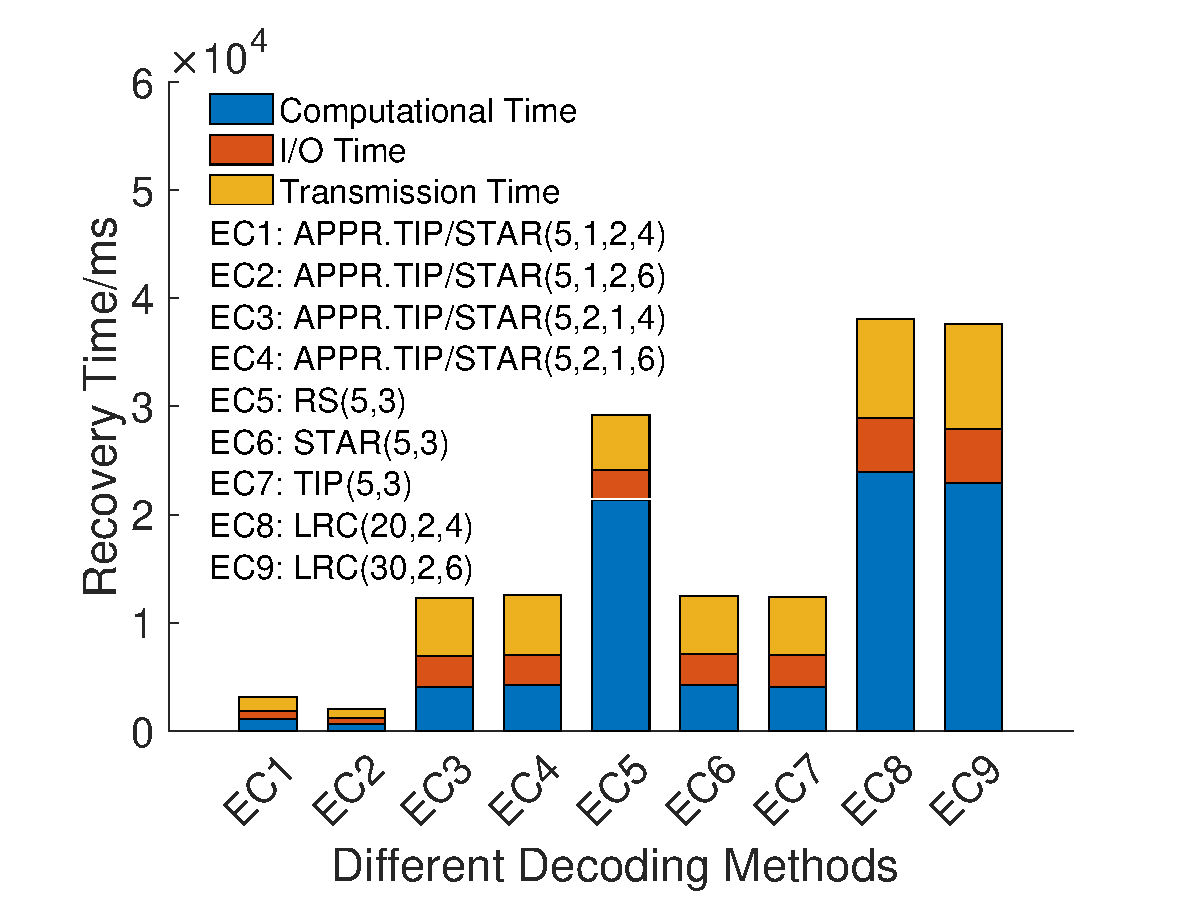
\includegraphics[width=0.5\linewidth]{photo/experiment/Recovery-2.eps}\label{fig-rec-2}
}\hspace{-0.4cm}
\subfigure{
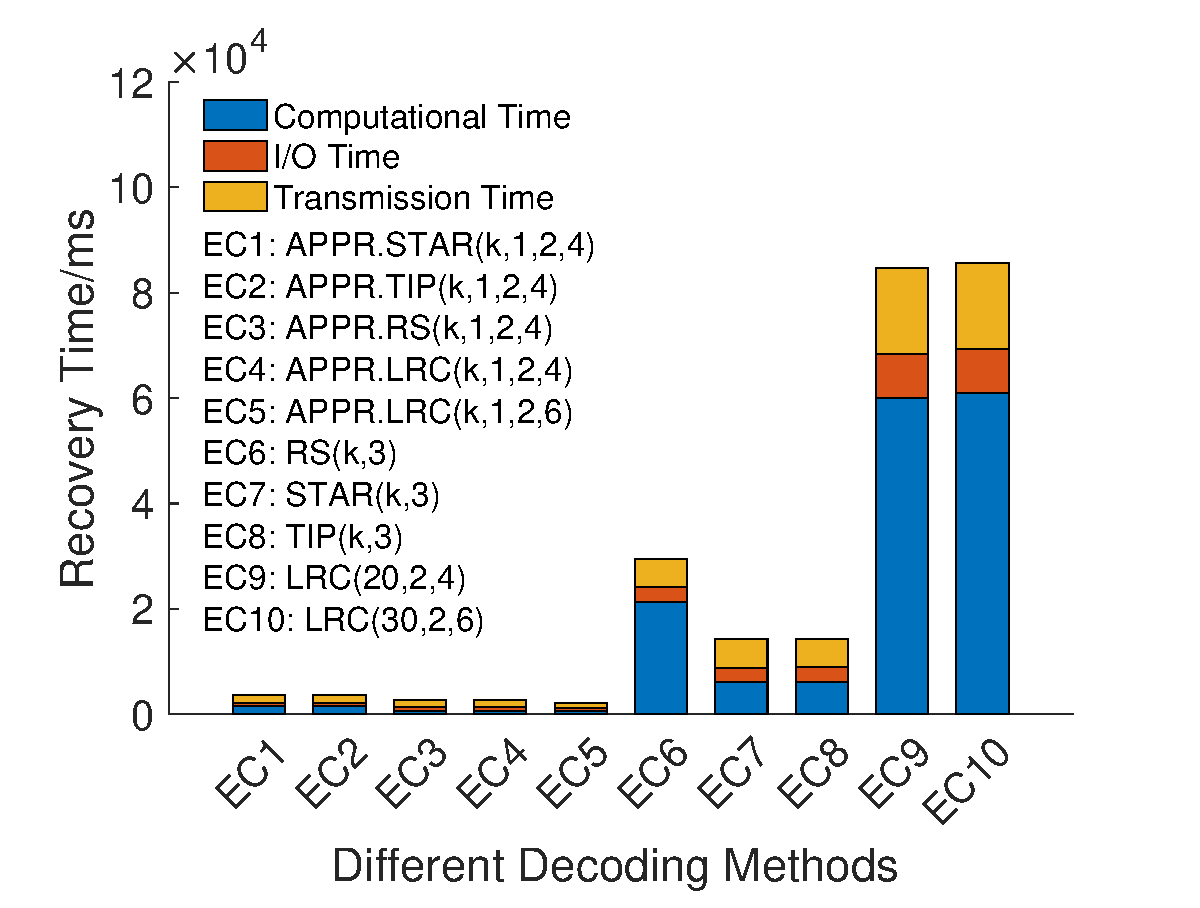
\includegraphics[width=0.5\linewidth]{photo/experiment/Recovery-3.eps}\label{fig-rec-3}
}
\caption{Recovery time Result using Frame Interpolation}
\label{fig-recoverytime}
\end{figure}

\section{Conclusion}\label{Conclusion}
In this paper, we present the Approximate Code, which is the framework for video tiered storage in cloud systems. The Approximate Code can segment the input erasure codes and provide different fault tolerance for data of different importance. For important data, the Approximate Code provides 3DFTs, and for non-critical data, the Approximate Code provides single or double parity, thus saving storage costs and speeding up recovery, while having good update write performance. We conducted several experiments in the Hadoop system and found that compared to traditional 3DFTs using various erasure codes such as RS, STAR and TIP-Code, Approximate Code reduces the number of parities by up to 55\%, saves the storage cost by up to 20.8\%, increase the recovery speed by up to 1.25X when single disk fails, and can reconstruct the whole video data via fuzzification when triple disks fail.

\bibliographystyle{ACM-Reference-Format}
\bibliography{ApproximateCode}

\end{document}
